\documentclass[10pt]{article}

% Preamble

\usepackage{amsmath,amsfonts,amssymb}
\usepackage[mathscr]{euscript}
%\usepackage[mathcal]{euscript}
\usepackage{mathrsfs}
\usepackage{graphicx}
\usepackage{float}
\usepackage{bbm}
\usepackage{braket}
\usepackage{tikz-feynman}
\usepackage{simpler-wick}
\usepackage{cancel}
\usepackage{stackengine}
\usepackage{slashed}
\usepackage{caption}
\usepackage{pgfplots}
\usepackage[colorlinks]{hyperref}
\hypersetup{linktocpage=true}

\newcommand{\bigzero}{\mbox{\normalfont\Large\bfseries 0}}

\title{Notes On Advanced Quantum Field Theory \\ The Theory of Elementary Interactions \\ A Course Given By Dr. Tobias Osborne}
\author{Transcribed by Dr. Alexander V. St. John}

% The Document

\begin{document}

\maketitle

\clearpage

{\hypersetup{linkcolor=blue}\tableofcontents} % Table of contents with clickable links.
\newpage

\section{Lecture 1: Introduction}
\label{sec: lec1}

\noindent The goal for this course is to explain the current "standard model" for particle physics. This is too lofty of a goal for this course, so what we focus on is the textit{building blocks} of the standard model, such that we understand the origin and purpose of each term of the Lagrangian. \\

\noindent Topics covered include

\begin{enumerate}
\item Path integral quantization
	\subitem Via Gaussian integrals.
\item Review perturbation theory via path integrals
	\subitem Includes familiar tools for calculating correlation functions such as Wick's theorem, Feynman rules, etc.
\item Renormalization
	\subitem Allows us to discuss effective QFT (e.g., eliminating infinities) in more detail.
\item Abelian and nonabelian classical gauge theories
	\subitem Uses path integrals to deduce quantizations from classical field theories.
\item Quantization of non-abelian gauge theories
	\subitem Employs path integrals for perturbative calculations and lattices for nonperturbative calculations.
\item Spontaneous symmetry breaking mechanisms
\end{enumerate}

\subsection*{Path Integrals}

\noindent Let's first suppose that the quantization is already done, and we have a quantum system with a Hilbert space $\mathcal{H}$, a Hamiltonian $\hat{H}$, and a propagator from integrating the Schroedinger equation, $U(t) = e^{-i\hat{H}t}$. \\

\noindent Now work out a representation to first order for the propagator by Taylor expanding

\begin{equation}
U(t) = e^{-i\hat{H}t} = \left( e^{-\frac{it}{N}\hat{H}}  \right) ^N= \lim_{N \rightarrow \infty} \left( \mathbb{I} - \frac{it}{N}\hat{H} \right) ^N
\end{equation}

\noindent Let $\{ \ket{j} \}$ be a basis for the Hilbert space $\mathcal{H}$ and consider the transition amplitude of evolving from an eigenstate $\ket{\phi_i}$ to another eigenstate $\ket{\phi_f}$

\begin{equation}
\bra{\phi_f} U(t) \ket{\phi_i} = \bra{\phi_f}  \left( e^{-\frac{it}{N}\hat{H}}  \right) ^N \ket{\phi_i}
\end{equation}

\noindent Insert  $N-1$ Hilbert space basis completeness relations, one in between each of the $N$ exponentials, and note that the sum over all paths from initial state to final state of functions of the paths

\begin{align}
\bra{\phi_f} U(t) \ket{\phi_i} &= \sum_{j_1,\dots,j_{N-1}} \bra{\phi_f} e^{-\frac{it}{N}\hat{H}} \ket{j_{N-1}}\bra{j_{N-1}} e^{-\frac{it}{N}\hat{H}} \dots \ket{j_1}\bra{j_1} e^{-\frac{it}{N}\hat{H}} \ket{\phi_i} \\
&\equiv \sum_{\text{paths}} f(j_1, \dots , j_{N-1}).
\end{align}

\noindent So, the transition amplitude of this state evolution is a sum over all of the paths through the basis states $j_1,\dots,j_{N-1}$. An example schematic of a path is visualized below.

\begin{figure}[H]
	\centering
	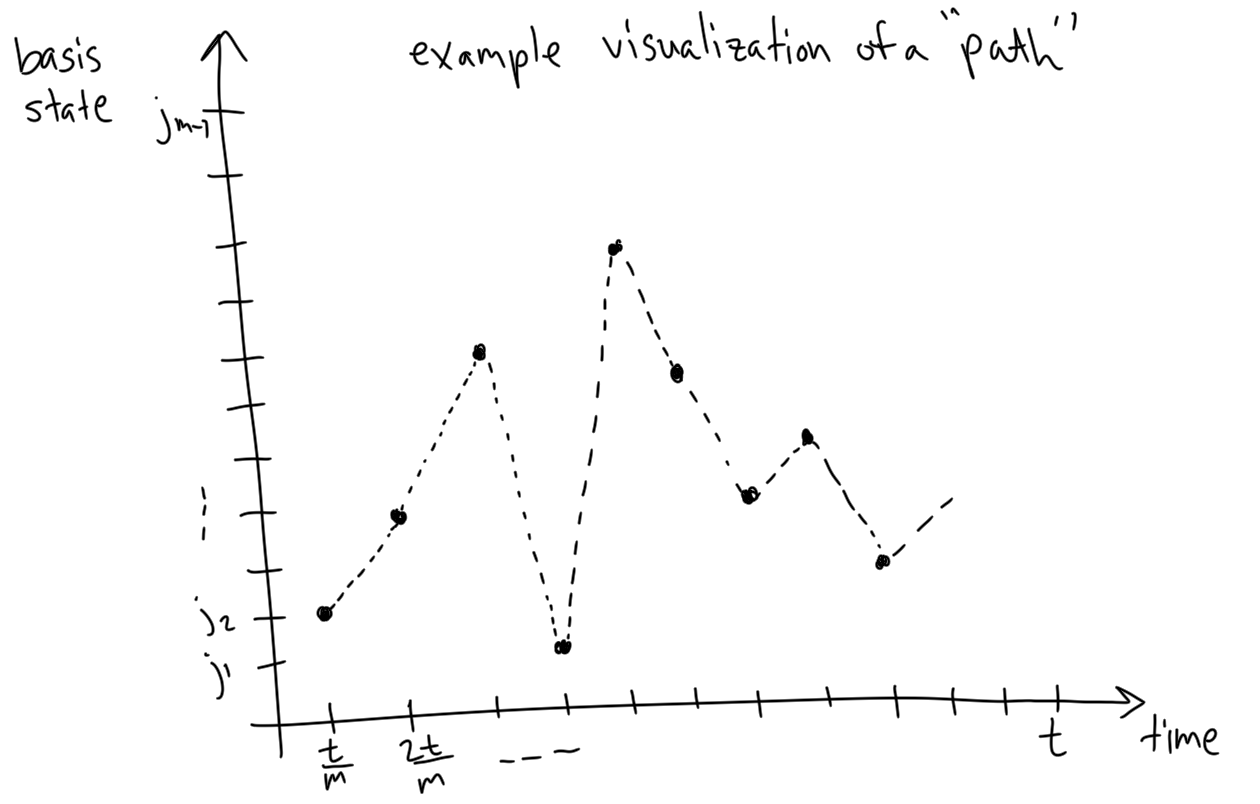
\includegraphics[width=4in]{images/pathviz.png}
	\caption*{}
\end{figure}

\noindent To work out the function of the path $f(j_1, \dots, j_{N-1})$, we need to calculate these individual transition amplitudes between successive states $\ket{j_{k-1}}$ to some final state $\bra{j_k}$ in the path integral setting, and seek to write it as an exponential of some function of the states $\mathcal{L}(j_{k-1}, j_k)$, the Lagrangian density

\begin{equation}
\bra{j_k} (\mathbb{I} - \frac{it}{N} \hat{H}) \ket{j_{k-1}} \simeq e^{\frac{it}{N} \mathcal{L}(j_{k-1}, j_k)}.
\end{equation}

\noindent So, the full transition amplitude will be a product of exponentials pf Lagrangian densities, well-known classical quantities

\begin{equation}
\bra{\phi_f} U(t) \ket{\phi_i} = \sum_{\text{paths}} f(j_1, \dots , j_{N-1}) = \sum_{j_1,\dots,j_{N-1}} e^{\frac{it}{N} \sum_{k=2}^{N-1} \mathcal{L} (j_{k-1}, j_k) } .
\end{equation}

\noindent Before moving forward, what makes the path integral so interesting?

\begin{enumerate}
\item It allows the calculation of quantum quantities, the transition amplitudes, via well-understood classical solutions and methods for handling highly oscillatory integrals such as the saddle point method.
\item It can also be used to build nonperturbative approximation schemes, such as Monte Carlo sampling over paths.
\end{enumerate}

\subsection*{Example: General Nonrelativistic Quantum Mechanical System}

\noindent Let's assume a little bit more about our quantum system. Suppose the quantum system is inspired by a classical system with pairs of canonical coordinates and momenta and the Hamiltonian $H(\{q^j\},\{p^j\}) = H(q,p)$. \\

\noindent Turn around the path integral sum over paths to guess a quantum Hamiltonian and Hilbert space from this classical Hamiltonian via

\begin{equation}
U(q_i, q_f, T) = \bra{q_f} U(T) \ket{q_i} = \bra{q_f} e^{-iT\hat{H}} \ket{q_i}
\end{equation}

\noindent Proceed as before, mulitplying the exponentials and inserting $N-1$ completeness relations in between the $N$ copies of the exponential. The completeness relation for the canonical position basis, a continuous variable, is

\begin{equation}
\mathbb{I} = \left( \prod_j \int dq_k^j \right) \ket{q_k} \bra{q_k}
\end{equation}

\noindent So, the transition amplitude in this case is, with $\epsilon \equiv \delta t = \frac{T}{N}$

\begin{equation}
\bra{q_f} U(T) \ket{q_i} = \sum_{k_1,\dots,k_{N-1}} \bra{q_f} e^{-i \epsilon \hat{H}} \ket{q_{k_{N-1}}} \bra{q_{k_{N-1}}} \dots \ket{q_{k_1}}\bra{q_{k_1}} e^{-i \epsilon \hat{H}} \ket{q_i}.
\end{equation}

\noindent There are three cases for the dependence of the quantum Hamiltonian on the canonical coordinates in the expression for the propagator. It can depend purely on position, purely on momenta, or most realistically, it can depend on both. \\

\noindent In the case that the Hamiltonian is a function purely dependent on canonical position, such that $\hat{H} = g(\hat{q})$, we easily calculate the transition amplitude, which relates the quantum and classical canonical positions, since the $\ket{q_k}$ are energy eigenstates of the position-dependent Hamiltonian

\begin{align}
\bra{q_{k+1}} g(\hat{q}) \ket{q_k} &= g(q_k) \prod_j \delta ( q_k^j - q_{k+1}^j ) \\
&= g \left( \frac{q_{k+1} + q_k}{2} \right) \left( \prod_j \int \frac{dp_k^j}{2\pi} \right) e^{ i \sum_j p_k^j (q_{k+1}^j - q_k^j ) }.
\end{align}

\noindent Where we used the Dirac delta distribution identity $\delta (q) = \int_{-\infty}^{\infty} \frac{dp}{2\pi} \, e^{i p \cdot q}$ to introduce the canonical momenta into the transition amplitude. Also note that the Dirac delta function forces $q_{k+1} = q_k$, such that $f(q_k) = f(\frac{q_{k+1} + q_k}{2})$, and we write it in this fashion for later use. \\

\noindent Next, in the case that the Hamiltonian is a function purely dependent on canonical momenta, such that $\hat{H} = h(\hat{p})$, the transition amplitude is calculated by inserting the completeness relation for the momentum eigenbasis.

\begin{align}
\bra{q_{k+1}} h(\hat{p}) \ket{q_k} &= \bra{q_{k+1}} h(\hat{p}) \cdot \prod_j \int dp_k^j \ket{p_k} \braket{p_k | q_k} \\
&= \prod_j \int \frac{dp_k^j}{2\pi} \, h(p_k) e^{ i \sum_j p_k^j (q_{k+1}^j - q_k^j ) }
\end{align}

\noindent Where the inner product of the position and momentum eigenstates is a Fourier phase element $\braket{p | q} = \frac{1}{2\pi} e^{i p \cdot q}$, and we get the sum, since the subscript $k$ denotes $N$ total canonical coordinate pairs. \\

\noindent The more realistic situation is when the Hamiltonian is dependent on both position and momenta $\hat{H} = \hat{H}(\hat{q}, \hat{p}) = g(\hat{q}) + h(\hat{p})$. Suppose the dependencies are linearly separable in the quantum Hamiltonian. Then we may translate between classical position and momenta via the Taylor expansion to first order

\begin{equation}
e^{-i \epsilon \hat{H}} = \mathbb{I} - i \epsilon \hat{H} = \mathbb{I} - i \epsilon (g(\hat{q}) + h(\hat{p})).
\end{equation}

\noindent Using this linearity, we can write this dependence in the derived formula as

\begin{equation}
\bra{q_{k+1}} e^{-i \epsilon \hat{H}(\hat{q}, \hat{p})} \ket{q_k} = \prod_j \int \frac{dp_k^j}{2\pi} \, e^{ -i \epsilon H (\frac{q_{k+1}+q_k}{2}, p_k)} e^{ i \sum_j p_k^j (q_{k+1}^j - q_k^j ) }
\end{equation}

\noindent Putting all this together into the propagator, which is really the transition amplitude for a nonrelativistic quantum system,

\begin{equation}
U(q_i, q_f; T) = \left(  \prod_{jk} \int dq_k^j \int \frac{p_k^j}{2\pi} \right) e^{i \sum_k \left( \sum_j p_k^j (q_{k+1}^j - q_k^j) - \epsilon H (\frac{q_{k+1} + q_k}{2}, p_k) \right)}.
\end{equation}

\noindent Take note that there is nothing quantum on the RHS: no hats! We have used purely classical data to define the quantum propagator, or, transition amplitude, on the LHS, such that $U(q_i, q_f; T) \propto e^{- i \epsilon H (q_i, q_f; T)}$. \\

\noindent A few other remarkable points:

\noindent Using the saddle point method, we can build an approximation scheme for $U$. This is useful for solving highly oscillatory integrals, as we see in the transition amplitude above (e.g., $e^{i\dots}$), since such integrals can be approximated by its saddle points (or critical points), which correspond to classical paths of the system. \\

\noindent Monte Carlo sampling of the system can also be used to approximate the transition amplitude by building an estimator for the RHS, sampling over classical configurations, and summing up the estimator. \\

\noindent Now, the expression for $U$ was not-so-pretty, but imagine continuous time variables and integrals when you see $\sum_k$ and $\epsilon$ above. In the limit as $N \rightarrow \infty$ (the number of completeness relations inserted), the quantum propagator is expressed in a continuous form with strange new "integrals".

\begin{equation}
U(q_i, q_f; T) = \left( \int \mathcal{D}q \int \mathcal{D} p \right) e^{i \int_0^T dt \, (\sum_j p^j \dot{q}^j - H(q,p))}
\end{equation}

\noindent Do not think of these as literal integrals, as we do not have a proper measure space to integrate over. Think of them as algorithms for now, something totally new that will be applied to solve this expression above.

\clearpage

\section{Lecture 2: Gaussian Path Integrals}
\label{sec: lec2}

\noindent Recall the propagator, or transition amplitude, for a nonrelativistic quantum system

\begin{equation}
U(q_i, q_f; T) = \left( \prod_j \int \mathcal{D} q^j (t) \int \mathcal{D} p^j (t) \right) e^{i \int^T_0 dt \, \mathcal{L} (q^j, \dot{q}^j)}.
\end{equation}

\noindent To work with this, we often discretize $q(t) \rightarrow q^j_k$

\begin{figure}[H]
	\centering
	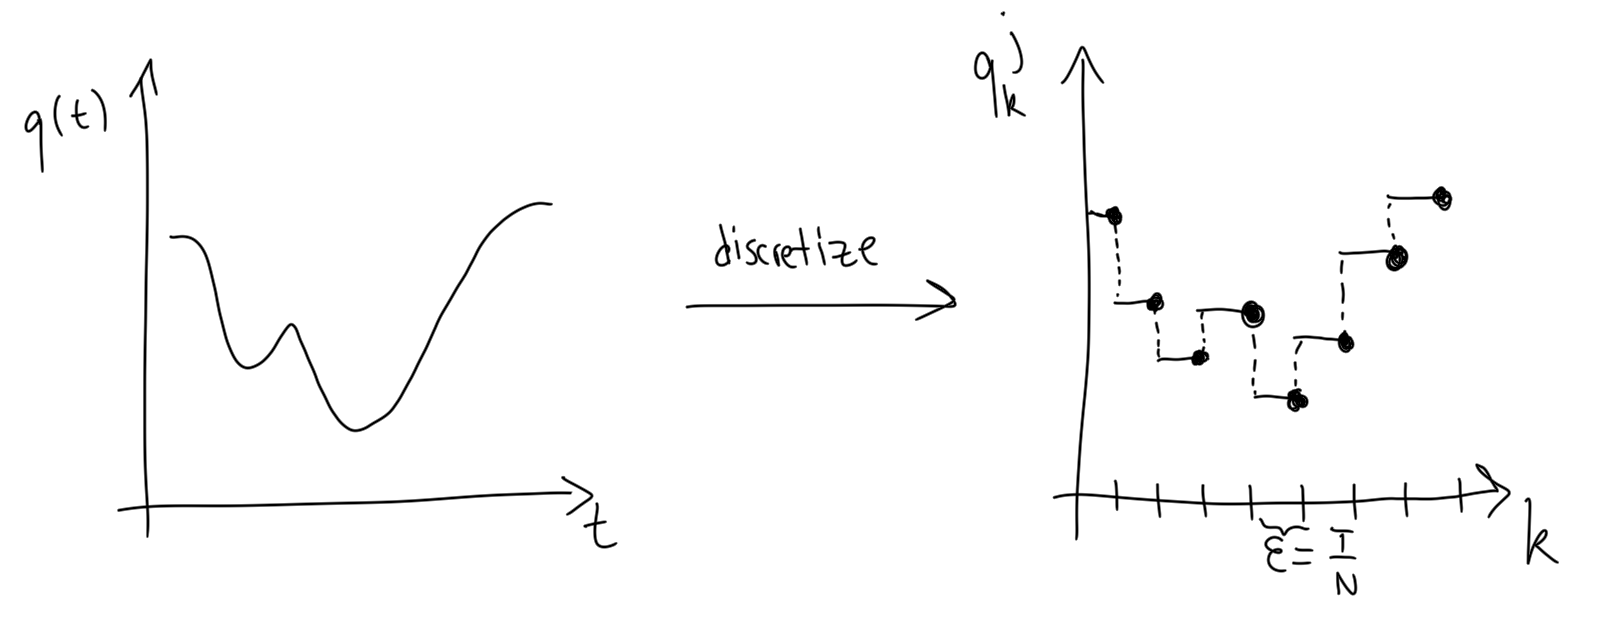
\includegraphics[width=4in]{images/discretize.png}
\end{figure}

\begin{equation}
U(q_i, q_f; T) = \left( \prod_{j, k} \int dq^j_k \int \frac{dp^j_k}{2\pi} \right) e^{i \sum_k (\sum_j p_k^j (q_{k+1}^j - q_k^j ) - \epsilon H)}
\end{equation}

\noindent Evaluate these very many integrals to get an answer dependent on $\epsilon = \frac{T}{N}$, since we discretized, take the limit as $\epsilon \rightarrow 0$ and deal with any encountered infinities.

\subsection*{Key Example}

\noindent Consider the classical Hamiltonian

\begin{equation}
H = \frac{p^2}{2 m} + V(q).
\end{equation}

\noindent Calculate the transition amplitude (\textbf{Exercise})

\begin{align}
U(q_i, q_f; T) &= \left( \prod_{j, k} \int dq^j_k \int \frac{dp^j_k}{2\pi} \right) e^{i \sum_k (\sum_j p_k^j (q_{k+1}^j - q_k^j ) - \epsilon H)} \\
&=  \left( \prod_{k} \int dq_k \int \frac{dp_k}{2\pi} \right) e^{i \sum_k (p_k (q_{k+1} - q_k ) - \epsilon (\frac{p_k^2}{2m} + V(q)) )} \\
&= \left( \prod_k \int dq_k \right) \sqrt{\frac{-im}{2\pi \epsilon}} e^{i \sum_k \frac{m}{2\epsilon} (q_{k+1} - q_k)^2 - \epsilon V\left(\frac{q_{k+1} + q_k}{2}\right)}.
\end{align}

\noindent We may also write this in the following notation, using the fact that the argument of the exponential is the discretized version of the action, now without the $p$-integral

\begin{equation}
\lim_{\epsilon \rightarrow 0} U(q_i, q_f; T) = \int \mathcal{D} q(t) e^{\mathcal{S}[q(t)]}
\end{equation}

\noindent Where the action is 

\begin{equation}
\mathcal{S}[q(t)] = \int^T_0 dt \,\, \left(\frac{m}{2} \sum_j (\dot{q}^j)^2 - V(q)\right).
\end{equation}

\noindent Note that if our system is a harmonic oscillator $V(q) = \frac{1}{2} m \omega^2 q^2$, we can do the full integral.

\subsection*{Path Integrals for Scalar Fields}

\noindent Recall the classical scalar field with Lagrangian density and Hamiltonian

\begin{align}
\mathcal{L} &= \frac{1}{2} (\partial_\mu \phi)^2 - V(\phi) \\
H &= \int d^3 x \,\, \left(\frac{1}{2} \pi^2(x) + \frac{1}{2} (\nabla \phi(x))^2 + V(\phi(x)) \right).
\end{align}

\noindent The path integral prescription for quantum scalar fields gives the transition amplitude, by blind application of the above, we conjecture that

\begin{equation}
\bra{\phi_b} e^{-i \hat{H} T} \ket{\phi_a} = \left( \int \mathcal{D} \phi \int \mathcal{D} \pi \right) e^{i \int^T_0 d^4x \, (\pi \dot{\phi} - H(\phi))}
\end{equation}

\noindent Where the boundary terms are $\phi(t=0, x) = \phi_a (\textbf{x})$ and $\phi(t=T, x) = \phi_b (\textbf{x})$. \\

\noindent As explained above, to make sense of this quantity, we must discretize, evaluate, and take the continuum limit as $\epsilon \rightarrow \infty$. When we discretize, note that we only discretize space, as discretizing time in this way will cause trouble with the conjugate momenta. \\

\noindent The field operators are discretized over a "grid" of points $x_j$ each of width $\epsilon$, such that

\begin{equation}
\phi(t, x) \,\,\, \rightarrow \,\,\, \phi(t, x_j) \equiv q^j (t).
\end{equation}

\noindent Then discretize the integral by turning it into a sum over the grid

\begin{equation}
\int d^3 x  \,\,\, \rightarrow \,\,\, \epsilon^3 \Sigma_{j \in \mathbb{Z}^3} .
\end{equation}

\noindent Next the derivative can be discretized via a finite difference. Note that there are more computationally efficient symmetric differences that can be used to discretize the derivative, but the finite difference works well for demonstration

\begin{equation}
\nabla_\mu \phi(x) \,\,\, \rightarrow  \,\,\, \frac{(\phi(x_j + \epsilon_\mu) - \phi(x_j))}{|\epsilon_\mu|}
\end{equation}

\noindent Where $\mu$ denotes the four directions in which to calculate the derivative

\begin{equation}
\epsilon_{\mu} = \epsilon \{ \left(\begin{smallmatrix}1\\0\\0\\0\end{smallmatrix}\right), \left(\begin{smallmatrix}0\\1\\0\\0\end{smallmatrix}\right), \left(\begin{smallmatrix}0\\0\\1\\0\end{smallmatrix}\right), \left(\begin{smallmatrix}0\\0\\0\\1\end{smallmatrix}\right) \}
\end{equation}.

\noindent Lastly, the potential just becomes evaluated at each $x_j$

\begin{equation}
V(\phi(x)) \,\,\, \rightarrow \,\,\, V(\phi(x_j)).
\end{equation}

\noindent Then the Lagrangian is discretized to a sum over a bunch of terms, but the only relevant term to the construction of the Hamiltonian is the time derivative of the field operator $\dot{\phi}$ (\textbf{Exercise})

\begin{equation}
L = \int d^3 x \, \mathcal{L} \rightarrow \epsilon^3 \sum_j \frac{1}{2} (\dot{\phi}_j)^2
\end{equation}

\noindent And the discretized conjugate momentum becomes

\begin{equation}
\pi^j = \frac{\partial L}{\partial \dot{q}^j} = \frac{\partial L}{\partial \dot{\phi}^j}  \,\,\, \rightarrow \,\,\, \epsilon^3 \dot{q}^j .
\end{equation}

\noindent Finally, we have the discretized Hamiltonian, where we display the $\epsilon$ terms to show that if we did not add the $\epsilon^3$ term to the discretized Lagrangian, we would be stuck with an extra $\epsilon^{-3}$ on the discretized Hamiltonian

\begin{equation}
H = \epsilon^3 \sum_j \epsilon^{-3} \pi_j^2 + \frac{1}{2} \left( \frac{q_{j+\epsilon^\mu}-q_j}{\epsilon} \right)^2 + V(q).
\end{equation}

\noindent In summary, the discretization of the scalar field gives us a nonrelativistic lattice system such that the discretized Hamiltonian is the sum of a kinetic energy term and a potential energy term. The second step is to evaluate the (nonrelativistic) path integral, and the third step is to take the continuum limit as $\epsilon \rightarrow 0$, which will later be re-branded as renormalization. \\

\noindent The most important case of the scalar field is the quadratic potential, which corresponds to the Klein-Gordon field (e.g., discretizing Klein-Gordon theory yields the quadratic potential below), is

\begin{equation}
V(q) = \frac{1}{2} q^T \textbf{A} q.
\end{equation}

\subsection*{Gaussian Integrals}

\noindent Consider the following integral 

\begin{equation}
I = \int_{-\infty}^\infty dx \,\, e^{-x^2} = \sqrt{\pi}.
\end{equation}

\noindent Proof:

\begin{align}
I &= \int_{-\infty}^\infty dx \,\, e^{-x^2} \\
I^2 &= \left(\int_{-\infty}^\infty dx \,\, e^{-x^2} \right) \left( \int_{-\infty}^\infty dy \,\, e^{-y^2}  \right) \\
I^2 &= \int_0^\infty r dr \, \int_0^{2\pi} d\theta \, e^{-r^2} \\
I^2 &= 2 \pi \int_0^\infty \frac{d}{dr} \left( -\frac{1}{2} e^{-r^2} \right) dr = \pi
\end{align} .

\noindent This is actually a special case of the more general forms of the Gaussian integral

\begin{align}
\int_{-\infty}^\infty dx \,\, e^{ -\frac{1}{2} a x^2 + b x } &= \sqrt{\frac{2\pi}{a}} e^{ \frac{b^2}{2a}  } \\
\int_{-\infty}^\infty dx \,\, e^{  i a x^2 + i b x } &= \sqrt{\frac{2\pi i}{a}} e^{ \frac{-i b^2}{2a}  } \\
\end{align}.

\noindent We will later need the moments generated by the Gaussian integral

\begin{align}
\langle x^n \rangle = \frac{\int_{-\infty}^\infty dx \,\, x^n e^{ -\frac{1}{2} a x^2}}{\int_{-\infty}^\infty dx \,\, e^{ -\frac{1}{2} a x^2}}.
\end{align}

\noindent Note that if $n$ is odd, then the moment is zero and we can write the exponent of $x$ as $2m$, where $m \in \mathbb{Z}$, and we have the relation (\textbf{Exercise})

\begin{equation}
\langle x^{2m} \rangle = \frac{(2m-1)!!}{a^m}.
\end{equation}

\noindent Note that the double factorial $(2m-1)!!$ represents the number of ways to join $2m$ points in pairs. -- "All science should in linear algebra or combinatorics." -- \\

\noindent Another closed form of this integral is in terms of derivatives is

\begin{align}
\langle x^{2m} \rangle &=  \left( \frac{d}{db} \right)^{2m} \left(  \frac{\int_{-\infty}^\infty dx \,\, e^{ -\frac{1}{2} a x^2 + b x }}{\int_{-\infty}^\infty dx \,\, e^{ -\frac{1}{2} a x^2 }} \right) \big|_{b=0} \\
\langle x^{2m} \rangle &= \left( \frac{d}{db} \right)^{2m} e^{\frac{b^2}{2a}} \big|_{b=0}.
\end{align}

\noindent To evaluate the maultivariable Gaussian integrals, where $x \in \mathbb{R}^n$, consider

\begin{equation}
I(\textbf{A}, B) = \int_{-\infty}^\infty dx_1 \dots \int_{-\infty}^\infty dx_n \,\, e^{-x^T \textbf{A} x + B^T x}
\end{equation}

\noindent Where $\textbf{A}$ is an $n \times n$ symmetric real matrix and $B$ is an $n \times 1$ real vector. Since $\textbf{A}$ is real, symmetric, it contains orthogonal $\textbf{O}$ and diagonal matrices $\textbf{D}$, such that $\textbf{O}^T \textbf{O} = \mathbb{I}$ and $\textbf{D}$ is diagonalized with the eignevalues of $\textbf{A}$.

\begin{equation}
\textbf{O}^T \textbf{D} \textbf{O} = \textbf{A}
\end{equation}

\noindent Assume that $B=0$ and define $y = \textbf{O} x$. Then

\begin{align}
I(\textbf{A}, B=0) &= \int_{-\infty}^\infty dy_1 \dots \int_{-\infty}^\infty dy_n \,\, e^{-y^T \textbf{D} y} \\
&= \prod_{j=1}^n \int_{-\infty}^\infty dy_j \,\, e^{-y_j^2 \lambda_j} \\
&= \prod_{j=1}^n \sqrt{\frac{\pi}{\lambda_j}} \\
I(\textbf{A}, B=0)&= \sqrt{\frac{\pi^n}{\text{det}(\textbf{A})}}.
\end{align}

\noindent The $B \ne 0$ case (\textbf{Exercise}) results in the following

\begin{equation}
I(\textbf{A},B) = \sqrt{\frac{\pi^n}{\text{det}(\textbf{A})}} e^{B^T \textbf{A}^{-1} B}.
\end{equation}

\clearpage

\section{Lecture 3: Correlation Functions and Path Integrals}
\label{sec: lec3}


\noindent Recall the generating function for a single-variable Gaussian probability distribution $e^{\frac{1}{2} a x^2}$ and the moment-generating integral

\begin{equation}
I = \int_{-\infty}^\infty dx \,\, x^{2n} e^{\frac{1}{2} a x^2} = \frac{(2n-1)!!}{a^n}.
\end{equation}

\noindent We also derived the identity with the generating function for the multivariable Gaussian probability distribution

\begin{equation}
\int_{-\infty}^\infty dx_1 \dots \int_{-\infty}^\infty dx_n \,\, e^{-\frac{1}{2} x^T \textbf{A} x + J^T x} = \sqrt{\frac{\pi^n}{\text{det}(\textbf{A})}} e^{J^T \textbf{A}^{-1} J}.
\end{equation}

\noindent The 2-point correlation function for the $n$-variable Gaussian is (\textbf{Exercise}), for $j \ne k$

\begin{equation}
\langle x_j x_k \rangle \equiv \frac{\int_{-\infty}^\infty dx_1 \dots \int_{-\infty}^\infty dx_n \,\, x_j x_k e^{-\frac{1}{2} x^T \textbf{A} x}}{\int_{-\infty}^\infty dx_1 \dots \int_{-\infty}^\infty dx_n \,\, e^{-\frac{1}{2} x^T \textbf{A} x}} \equiv[\textbf{A}^{-1}]_{jk}.
\end{equation}

\noindent Note that this is also equal to the second derivative with respect to the vector $J$, evaluated at $J=0$

\begin{equation}
\langle x_j x_k \rangle \equiv \frac{\frac{\partial^2}{\partial J_j \partial J_k}\int_{-\infty}^\infty dx_1 \dots \int_{-\infty}^\infty dx_n \,\, e^{-\frac{1}{2} x^T \textbf{A} x + J^T x} }{\int_{-\infty}^\infty dx_1 \dots \int_{-\infty}^\infty dx_n \,\, e^{-\frac{1}{2} x^T \textbf{A} x + J^T x}} \Big|_{J=0}.
\end{equation}

\subsection*{Higher Order Moments: $l$-point Correlation Functions}

\noindent The $l$-point correlation function has similar form

\begin{equation}
\langle x_{j_1} \dots x_{j_l} \rangle \equiv \frac{\int_{-\infty}^\infty dx_{j_1} \dots \int_{-\infty}^\infty dx_{j_l} \,\, x_{j_1} \dots x_{j_l} \,\, e^{-\frac{1}{2} x^T \textbf{A} x}}{\int_{-\infty}^\infty dx_{j_1} \dots \int_{-\infty}^\infty dx_{j_l} \,\, e^{-\frac{1}{2} x^T \textbf{A} x}}.
\end{equation}

\noindent By Wick's theorem (proof by induction), for even $l$, the $l$-point correlation function is proportional to the sum of the products over the permutation group on $l$ symbols, the "Wick sum". We write "proportional to" for reasons of symmetry and soon eliminating redundant terms.

\begin{equation}
\langle x_{j_1} \dots x_{j_l} \rangle \propto \sum_{\pi \in S_l} [\textbf{A}^{-1}]_{ j_{\pi^{-1}(1)}j_{\pi^{-1}(2)}} \dots [\textbf{A}^{-1}]_{j_{\pi^{-1}(l-1)}j_{\pi^{-1}(l)}} .
\end{equation}

\subsubsection*{Example: 4-point Correlation}

\noindent To calculate the 4-point correlation function, we begin by considering the $4!=24$ total permutations on 4 symbols. Since $\textbf{A}^{-1}$ is symmetric

\begin{equation}
[\textbf{A}^{-1}]_{jk} = [\textbf{A}^{-1}]_{kj} 
\end{equation}

\noindent And there are only $\frac{24}{2! 2! 2!} = 3$ unique terms (products of two matrix elements), which are (\textbf{Exercise})

\begin{align*}
\langle x_{j_1} x_{j_2} x_{j_3} x_{j_4} \rangle &= [\textbf{A}^{-1}]_{j_1 j_2} [\textbf{A}^{-1}]_{j_3 j_4} \\
&+ [\textbf{A}^{-1}]_{j_1 j_3} [\textbf{A}^{-1}]_{j_2 j_4} \\
&+ [\textbf{A}^{-1}]_{j_1 j_4} [\textbf{A}^{-1}]_{j_2 j_3} \\
&= \langle x_{j_1} x_{j_2} \rangle \langle x_{j_3} x_{j_4} \rangle + \langle x_{j_1} x_{j_3} \rangle \langle x_{j_2} x_{j_4} \rangle + \langle x_{j_1} x_{j_4} \rangle \langle x_{j_2} x_{j_3} \rangle
\end{align*}

\noindent With the approporiate choice of $\textbf{A}$, in the context of path integrals and perturbative field theory, these products of correlations functions are exactly correspondent to Feynman propagator, and, in turn, the Feynman diagrams, just as we studied in \textit{Lecture 9} of the last lecture series (Quantum Field Theory) for the 4-particle Wick contraction.

\begin{figure}[H]
	\centering
	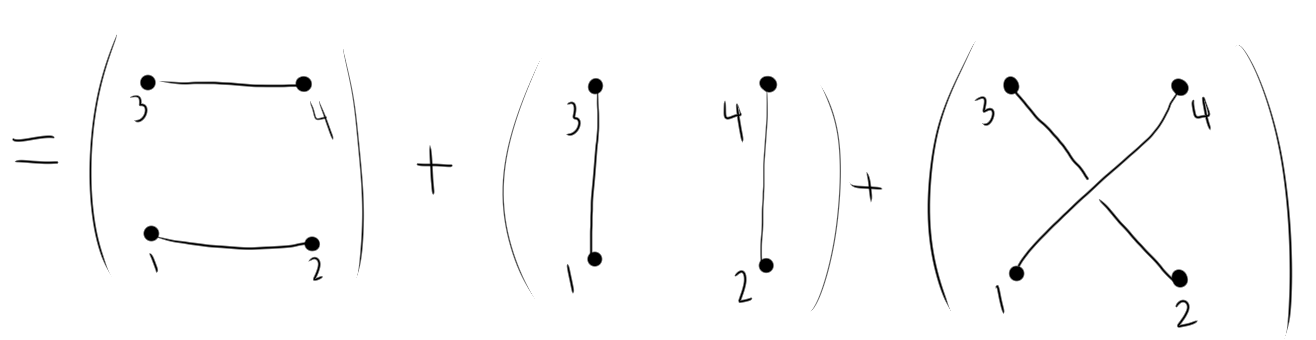
\includegraphics[scale=0.5]{images/feynman4point.png}
	\caption{Feynman diagram correspondence  of the 4-point correlation function}
\end{figure}

\noindent Keeping only unique terms, the proprotionality relation becomes an equivalence

\begin{equation}
\langle x_{j_1} \dots x_{j_l} \rangle  = \sum_{\text{unique} \,\pi^{-1}} [\textbf{A}^{-1}]_{ j_{\pi^{-1}(1)}j_{\pi^{-1}(2)}} \dots [\textbf{A}^{-1}]_{j_{\pi^{-1}(l-1)}j_{\pi^{-1}(l)}} 
\end{equation}

\noindent (\textbf{Exercise}) Calculate the 6-point correlation function with $\frac{6!}{2! 2! 2!} = 90$ unique terms

\begin{equation}
\langle x_{j_1} x_{j_2} x_{j_3} x_{j_4} x_{j_5} x_{j_6} \rangle = [\textbf{A}^{-1}]_{j_1 j_2} [\textbf{A}^{-1}]_{j_3 j_4}  [\textbf{A}^{-1}]_{j_5 j_6} + \dots
\end{equation}

\noindent In short summary,

\begin{itemize}
\item We can calculate \textit{all} moments for the Gaussian probability distribution.
\item We have a diagrammatic calculus to calculate the $l$-point correlation functions, which end up being exactly the Feynman propagators/diagrams, with appropriate choice of $\textbf{A}$, and is the direct connection of quantum field theory and Gaussian integrals.
\end{itemize}

\subsection*{The Matrix \textbf{A} for Path Integrals}

\noindent Let the potential $V$ be quadratic in the canonical position coordinate per particle $q_k$ (e.g., a one-dimensional chain of oscillators), such that the transition amplitude, which will be discretized, evaluated, and limited $\epsilon \rightarrow 0$, from some state $q_a$ to another $q_b$ is

\begin{equation}
U(q_a, q_b; T) = \left( \prod_k \int \frac{dq_k}{c(\epsilon)} \right) e^{\frac{1}{2} i q^T \textbf{A} q}
\end{equation}

\noindent Where we know the quadratic form contains a kinetic energy term plus a potential energy term

\begin{equation}
q^T \textbf{A} q = \sum_k \left( m \frac{(q_{k+1} - q_k}{\epsilon}^2 - \epsilon V (\frac{q_{k+1} + q_k}{2}) \right).
\end{equation}

\noindent This results is $\textbf{A}$ as a \textit{tridiagonal} matrix for the kinetic energy term and a potential energy term which is a matrix with elements quadratic in $q$

\begin{equation}
\textbf{A} = 
\begin{bmatrix}
    \frac{2m}{\epsilon} & -\frac{m}{\epsilon} & 0 & \cdots & & & \\
    -\frac{m}{\epsilon} & \frac{2m}{\epsilon} & -\frac{m}{\epsilon} & 0 & \cdots & & \\
    0 & -\frac{m}{\epsilon} & \frac{2m}{\epsilon}& -\frac{m}{\epsilon}& 0 & \cdots \\
    \vdots & 0 &\ddots & \ddots & \ddots
\end{bmatrix}
+ [V( q^2 )]
\end{equation}

\noindent The transition amplitude is then calculated similarly to last lecture as

\begin{equation}
U(q_a, q_b; T) = \frac{ \infty \, \text{const.}}{\sqrt{\text{det}(\textbf{A})}}
\end{equation}

\noindent The infinite constant will not be a problem since the $l$-point correlation is normalized, and the same exact infinite constant will appear in the denominator and cancel the constant. So, in terms of $q_k$, the $l$-point correlation reads

\begin{equation}
\langle q_{j_1} \dots q_{j_l} \rangle \equiv \frac{\prod_k \int \frac{dq_k}{c(\epsilon)} q_{j_1} \dots q_{j_l} \,\, e^{-\frac{1}{2} i q^T \textbf{A} x}}{\prod_k \int \frac{dq_k}{c(\epsilon)} \,\, e^{-\frac{1}{2} i q^T \textbf{A} x}}.
\end{equation}

\noindent Note that with periodic boundary conditions, the elements of follow a modulo relation $\textbf{A}_{jk} = f((j-k) \, \text{mod} \, n)$, where $n$ is the number of sites/oscillators in the chain. \\

\noindent Assuming that $\textbf{A}$ is invertible, there exists a unitary matrix $Q$, such that $Q^T Q = \mathbb{I}$ and $Q^T \textbf{A} Q = D$, with diagonal matrix $D$ with the eigenvalues of $\textbf{A}$ along the diagonal. Then the determinant of $\textbf{A}$ is easy to calculate, since 

\begin{equation}
\text{det}(\textbf{A}) = \prod_{j=1}^n \lambda_j (\textbf{A}).
\end{equation}

\subsection*{Correlations Functions and Quantum Observables}

\noindent Consider the transition amplitude over 2-point spatial correlations

\begin{equation}
U(q_a, q_b; T) \propto \int \mathcal{D} \phi(x) \,\, \phi(x_1) \phi(x_2) e^{i \int_{-T}^T d^4 x \, \mathcal{L}(\phi)}
\end{equation}

\noindent With an expression like this, always discretize by sending $\phi(x_j) \rightarrow q_j$, evaluate the integral, and enter the contiuum limit with the boundary conditions

\begin{align}
\phi (-T, x) &= \phi_a (x) \\
\phi (T, x) &= \phi_b (x).
\end{align}

\noindent Apply the following condition, exploiting the boundary conditions, to factor the full field "integral" over the individual fields and the boundary of the field

\begin{equation}
\int \mathcal{D} \phi (x) = \int \mathcal{D} \phi_1 (x) \int \mathcal{D} \phi_2 (x) \int_{\partial \phi} \mathcal{D} \phi (x)
\end{equation}

\noindent Where the boundary $\partial \phi = \partial \phi_1 + \partial \phi_2$ is defined by 

\begin{align}
\phi_1 (x) = \phi(x_1^0, x_1) \\
\phi_2 (x) = \phi(x_2^0, x_2)
\end{align}

\noindent So, after performing the boundary integral, we introduce quantum stuff to the expression from the classical 2-point function above, for $x_2^0 > x_1^0$

\begin{align*}
U(q_a, q_b; T) \propto \int \mathcal{D} \phi_1 (x) \int \mathcal{D} \phi_2 (x) \,\, &\phi(x_1) \phi(x_2) \bra{\phi_b} e^{-i \hat{H} (T-x_2^0)} \ket{\phi_2} \\
 &\times \bra{\phi_2} e^{-i \hat{H} (x_2^0 - x_1^0)} \ket{\phi_1} \bra{\phi_1} e^{-i \hat{H} (x_1^0 + T)} \ket{\phi_a}
\end{align*}

\noindent Now, apply the Schroedinger-picture field operator to write the classical field operators in terms of quantum field operators. The formula is

\begin{equation}
\hat{\phi}_S (x) \ket{\phi_1} = \phi (x_1) \ket{\phi_1}
\end{equation}

\noindent So, the purely quantum expression for the 2-point function is

\begin{align*}
U(q_a, q_b; T) \propto\int \mathcal{D} \phi_1 (x) \int \mathcal{D} \phi_2 (x) \,\, &\bra{\phi_b} e^{-i \hat{H} (T-x_2^0)} \hat{\phi}_S (x) \ket{\phi_2} \\
 &\times \bra{\phi_2} e^{-i \hat{H} (x_2^0 - x_1^0)} \hat{\phi}_S (x) \ket{\phi_1} \bra{\phi_1} e^{-i \hat{H} (x_1^0 + T)} \ket{\phi_a}
\end{align*}

\noindent This is called the time-ordered expectation value of the field operators in the Heisenberg picture. The equation holds for $x_2^0 < x_1^0$ as well, and we can write it as

\begin{equation}
U(q_a, q_b; T) \propto \bra{\phi_b} e^{-i \hat{H} T} \mathcal{T}[ \hat{\phi}_H (x_1) \hat{\phi}_H (x_2)] e^{-i \hat{H} T} \ket{\phi_a}
\end{equation}

\noindent Now, enter the limit as $T \rightarrow \infty$, where we bring the interacting vacuum state and the normalization for the full transition amplitude (\textbf{Exercise}), and introduce the \textit{most important formula} for this course

\begin{equation}
\bra{\Omega} \mathcal{T} [ \hat{\phi}_H (x_1) \hat{\phi}_H (x_2) ] \ket{\Omega} = \lim_{T \rightarrow \infty (1-i\epsilon)} \frac{\int \mathcal{D} \phi \,\, \phi (x_1) \phi (x_2) e^{i \int_{-T}^T d^4 x \, \mathcal{L} (\phi)}}{\int \mathcal{D} \phi \,\, e^{i \int_{-T}^T d^4 x \, \mathcal{L} (\phi)}}.
\end{equation}

\noindent So, the LHS is built of purely quantum observables equal to the classical expression of path integrals! \\

\noindent This expression will end up to be the propagator, which is also the inverse of the Klein-Gordon operator, which is what we call $\textbf{A}$ in the scalar quantum field theory. \\

\noindent The solution to this is well-known for the case when $\mathcal{L}$ is quadratic in the field operators, and one can easily discretize, evaluate the Gaussian integral, and take the limit as $\epsilon \rightarrow 0$. \\

\noindent \textbf{(Exercise)} Calculate the $l$-point formula for the time-ordered expectation value of the field operators in the Heisenberg picture.

\clearpage

\section{Lecture 4: Functional Quantization of the Scalar Field}
\label{sec: lec4}

\noindent The path integral formalism for quantization of fields is an incredibly efficient tool, but one must learn when, and when not, ot use it. Through the lectures and many examples, we'll develop an intuition for when to trust quantization via path integrals. \\

\noindent Recall the action of the scalar field $S$ with classical field operators $\phi$

\begin{equation}
S_0 = \int d^4 x \,\, \mathcal{L}_0 = \int d^4 x \,\, \left( \frac{1}{2} (\partial_\mu \phi)^2 - \frac{1}{2} m^2 \phi^2 \right).
\end{equation}

\noindent We will (1) discretize, tantamount to imposing a cutoff $\Lambda$, (2) evaluate the integrals, and (3) enter the continuum limit where $\epsilon \rightarrow 0$. Start the discretization by putting the field on a lattice (a Lorentz manifold) with spacing $\epsilon$ and then compactify the space onto a torus for periodic boundary conditions.  \\

\noindent Mathematically, we are transforming from a four-dimensional Minkowski space $\mathcal{M}^4$ to a four-domensional torus $(\mathbb{Z}/N\mathbb{Z})^4$, where $N = \frac{L}{\epsilon}$ is the number of sites, and $L$ is the total size of grid.

%\begin{figure}[H]
%	\centering
%	\includegraphics[scale=0.5]{images/compactify.png}}
%\end{figure}

\noindent Continue discretization with the field operators

\begin{align}
\phi(x) \rightarrow &\phi(x_j) \equiv q_j, \\
&x_j=\epsilon j \in \frac{L}{N} (\mathbb{Z}/N\mathbb{Z})^4.
\end{align}

\noindent And the partial derivatives are replaced for the forward difference, which is not the best method, but it's "good enough for government work"

\begin{equation}
\partial_\mu \phi (x) \rightarrow \frac{\phi(x_j + \epsilon e^\mu) - \phi(x_j)}{\epsilon}.
\end{equation}

\noindent And the space-time integral becomes a sum over the sites on the torus

\begin{equation}
\int d^4 x \, \rightarrow \epsilon^4 \sum_{j \in (\mathbb{Z}/N\mathbb{Z})^4}
\end{equation}

\noindent Now following the path integral quanitzation recipe, consider the transition amplitude in terms of the discretized action

\begin{equation}
\bra{\phi_f} U(q_i, q_f; T) \ket{\phi_i} = \int \mathcal{D} \phi \,\, e^{i S_0}
\end{equation}

\noindent Where we follwo the "algorithm" of the integral-differential operator and discretize it to a product, over the torus sites, of integrals ($N^4$ total integrals) over the field operators, the canonical position variables 

\begin{equation}
\int \mathcal{D} \phi \rightarrow \prod_j \int d \phi (x_j) \equiv \prod_j \int d q_j.
\end{equation}

\subsection*{Discretization in Momentum Space}

\noindent Thus far we have worked entirely in real (position) space. Let's Fourier transform over into momentum space to continue discretization. The Fourier transform is a unitary transformation with Jacobian equal to 1 (\textbf{Exercise}). First, the field operators transform as

\begin{equation}
\phi (x_j) = \frac{1}{V} \sum_n e^{-i k_n \cdot x_j} \phi (k_n)
\end{equation}

\noindent Where $V=L^4$ is the volume of the 4D torus. Notationally, the $k$ argument to the field operator in momentum space $\phi (k)$ will denote the Fourier transform of the field operator in real space $\phi (x)$. The wavenumber $k_n$ is discretized over the torus as

\begin{equation}
k_n = \frac{2 \pi n^\mu}{L}, \,\, n^\mu \in \mathbb{Z}/N\mathbb{Z} \,\, \text{and} \,\, |k^\mu| < \frac{\pi}{\epsilon}
\end{equation}

\noindent Note that the Fourier space field operator is complex, such that $\phi(-k) = \phi^* (k)$, and we therefore have two independent variables per field operator in momentum space: the real part $\Re \phi (k_n)$ and the imaginary part $\Im \phi (k_n)$ for positive time-component $k_n^0 > 0$.

\noindent So, in momentum space, the discretized integral-differential operator is (\textbf{Exercise})

\begin{equation}
\int \mathcal{D} \phi = \prod_{n: k_n^0 > 0} \int d \, \Re \phi (k_n) \int d \, \Im \phi (k_n).
\end{equation}

\noindent And the discretized action for the scalar field in momentum space is (\textbf{Exercise})

\begin{equation}
S_0 = - \frac{1}{V} \sum_{k_n^0 > 0} (m^2 - k_n^2) ( (\Re \phi_n)^2 + (\Im \phi_n)^2)
\end{equation}

\noindent Where $\phi_n \equiv \phi(k_n)$, and the following relation for the Kronecker delta is used to obtain this expression

\begin{equation}
\delta_{k,0} = \frac{1}{n} \sum_{j=0}^{n-1} e^{\frac{2\pi i j k}{n}}.
\end{equation}

\noindent Our expression for the path integral for the Klein-Gordon field discretized to a lattice (four-dimensional with periodic boundary conditions) is comprised of Gaussian integarls over a finite number of degrees of freedom

\begin{equation}
I_0 = \int \mathcal{D} \phi \, e^{i S_0} = \left( \prod_{k_n^0 > 0} \int d \, \Re \phi_n \int d \, \Im \phi_n \right) e^{-i \frac{1}{V} \sum_{k_n^0 > 0} (m^2 - k_n^2 ) | \phi_n |^2}.
\end{equation}

\noindent Now, onto evaluating this integral, it's just a bunch of Gaussian integrals, and we know how to solve those. We get the following, and unrestrict $k_n$ to get the second line (\textbf{Exercise}) 

\begin{align}
I_0 &= \prod_{k_n^0 > 0} \sqrt{\frac{-i \pi V}{m^2 - k_n^2}} \cdot \sqrt{\frac{-i \pi V}{m^2 - k_n^2}} \\
I_0 &=  \prod_{k_n} \sqrt{\frac{-i \pi V}{m^2 - k_n^2}}
\end{align}

\noindent Note that $k_n$ is bounded, but we have an infinity when $V \rightarrow \infty$ (continuum limit), but this integral does not yet have full operational meaning and is proportional to the transition amplitude $I_0 \propto \bra{\phi_f} U(q_i, q_f; T) \ket{\phi_i}$, and the infinities will cancel and drop out in the full expression. \\

\subsection*{Heuristic Argument for $I_0$}

\noindent As the "surface area of knowledge" we need to remember the path integral formalism is small, there is a heuristic way to obtain this result without formal discretization, etc., using the aforementioned intuition. \\

\noindent Recall the Gaussian integral whose argument is quadratic in its independent variable

\begin{equation}
\int dx \,\, e^{-x^T \textbf{A} x} = \sqrt{\frac{\pi^n}{\text{det}(\textbf{A})}} \propto (\text{det}(\textbf{A}))^{-\frac{1}{2}}
\end{equation}

\noindent For the Klein-Gordon field, consider the path integral with the Klein-Gordon operator and field operators substituted

\begin{equation}
\int \mathcal{D} \phi \,\, e^{i S} \,\, \sim  \,\, \int \mathcal{D} \phi \,\, e^{\frac{1}{2} \int d^4 x \,\, \phi(x) (-\partial^2 - m^2) \phi (x)}
\end{equation}

\noindent So, we are boldly extrapolating to say that $\textbf{A}$ is like the Klein-Gordon operator and the $x$ is like the field operator

\begin{equation}
\int d^4 x \,\, \phi (x) (-\partial^2 - m^2) \phi (x) \sim x^T \textbf{A} x.
\end{equation}

\noindent Furthermore, we say that the path integral is proportional to the determinant of the Klein-Gordon operator

\begin{equation}
\int \mathcal{D} \phi \,\, e^{i S} \,\, \propto \,\, (\text{det}(-\partial^2 - m^2))^{-\frac{1}{2}}.
\end{equation}

\subsection*{Operationally Well-Defined Quantities}

\noindent As mentioned, $I_0$ cancels for operationally well-defined quanities, such as the 2-point correlation function, a time-ordered expectation value of products of the field operators. For example, using the path integral formalism

\begin{equation}
\bra{\Omega} \mathcal{T} [ \phi (x_1) \phi (x_2) ] \ket{\Omega} = \lim_{T \rightarrow \infty (1 - i \epsilon)} \frac{\int \mathcal{D} \phi \,\, \phi(x_1) \phi(x_2) e^{i S}}{\int \mathcal{D} \phi \,\, e^{i S}}
\end{equation}

\noindent To check our bold extrapolations, calculate the discretized field operator product

\begin{equation}
\phi (x_1) \phi (x_2) = \frac{1}{V^2} \sum_m e^{-i k_m \cdot x_1} \phi_m \sum_l e^{-i k_l \cdot x_2} \phi_l
\end{equation}

\noindent So, the discretized RHS numerator of the time-ordered expectation value above is just a bunch of  independent Gaussian integrals, quadratic in its independent variables (\textbf{Exercise})

\begin{align*}
\text{numerator} &= \frac{1}{V^2} \sum_{l,m} e^{-i (k_m \cdot x_1 + k_l \cdot x_2)} \left( \prod_{k_n^0 > 0} \int d \, \Re \phi_n \int d \, \Im \phi_n  \right) \\
&\,\,\,\,\,\, \times (\Re \phi_m + i \Im \phi_m ) (\Re \phi_l + i \Im \phi_l) e^{-i\frac{1}{V} \sum_{k_n^0 > 0} (m^2 - k_n^2 ) ((\Re \phi_n)^2 + (\Im \phi_n)^2)} \\
&= \frac{1}{V^2} \sum_m e^{-i k_m \cdot (x_1 - x_2)} \left( \prod_{k_n^0 > 0} \frac{-i \pi V}{m^2 - k_n^2} \right) \frac{-i V}{m^2 - k_n^2 - i \epsilon} \\
&= \frac{1}{V^2} \sum_m e^{-i k_m \cdot (x_1 - x_2)} \cdot I_0 \cdot \frac{-i V}{m^2 - k_n^2 - i \epsilon} 
\end{align*}

\noindent Where we drastically cut down the number of integrals to evaluate, since any integrals involving products like $\Re \phi_m \cdot \Im \phi_l$ or $\Im \phi_m \cdot \Re \phi_l$ form odd integrands and evaluate to zero. The integeral will also be zero for terms where $m \ne l$ and for terms where $k_m = k_l$. Integrals where $k_m = -k_l$ will \textit{not} be zero. \\

\noindent Bringing this together, the RHS of the time-ordered expectation value has boiled down to 

\begin{align}
\bra{\Omega} \mathcal{T} [ \phi (x_1) \phi (x_2) ] \ket{\Omega} &= \lim_{T \rightarrow \infty (1 - i \epsilon)} \frac{\int \mathcal{D} \phi \,\, \phi(x_1) \phi(x_2) e^{i S}}{\int \mathcal{D} \phi \,\, e^{i S}} \\
&= \lim_{V \rightarrow \infty} -i \frac{1}{V} \sum_n \frac{e^{-i k_n \cdot (x_1 - x_2) }}{m^2 - k_n^2 - i \epsilon} \\
&= \int \frac{d^4 k}{(2\pi)^4} \, \, \frac{i e^{-i k \cdot (x_1 - x_2)}}{-m^2 + k^2 + i \epsilon} \\
\bra{\Omega} \mathcal{T} [ \phi (x_1) \phi (x_2) ] \ket{\Omega} &= D(x_1 - x_2)
\end{align}

\noindent So, the path integral formalism gives us exactly the propagator we wish to see. Note that is we were to just boldy extrapolate, without discretization, etc., we would get the same result! \\

\noindent For example,

\begin{equation}
\frac{\int \mathcal{D} \phi \,\, \phi(x_1) \phi(x_2) e^{i S}}{\int \mathcal{D} \phi \,\, e^{i S}} = \frac{(\partial^2 - m^2)^{-\frac{1}{2}} D(x_1 - x_2)}{(\partial^2 - m^2)^{-\frac{1}{2}}}
\end{equation}

\noindent Since if $\textbf{A} \sim (-\partial^2 - m^2)$ \\
Then $[ \textbf{A}^{-1}]_{jk} \sim \frac{1}{(-\partial^2 - m^2)_{x_1 x_2}} = D(x_1 - x_2)$ \\
And  $\delta^{(4)} (x-y) = (-\partial^2 - m^2) D(x-y)$. \\

\subsection*{Example: 4-point Correlation Function}

\noindent Note that all 3-point correlations are zero, since they all have odd integrands. The 4-point correlation function starts off as

\begin{equation}
\bra{\Omega} \mathcal{T} [ \phi (x_1) \phi (x_2) \phi (x_3) \phi (x_4) ] \ket{\Omega} = \lim_{T \rightarrow \infty (1 - i \epsilon)} \frac{\int \mathcal{D} \phi \,\, \phi(x_1) \phi(x_2) \phi(x_3) \phi(x_4) e^{i S}}{\int \mathcal{D} \phi \,\, e^{i S}}.
\end{equation}

\noindent The numerator contains the quantities of $(\Re \phi_m + i \Im \phi_m) \dots (\Re \phi_l + i \Im \phi_l)$, and most terms will vanish as before, leaving us with terms where $k_l = -k_m$ and $k_q = -k_p$, and we end up with, after applying Wick's theorem and sending $V \rightarrow \infty$ (\textbf{Exercise}), something like

\begin{align*}
&\sum_{k_l, k_q} e^{-i \dots} \int \dots \phi_{k_l} \phi_{-k_l} \phi_{k_q} \phi_{-k_q} e^{\dots} \\
&= D_F(x_1 - x_2) D_F (x_3 - x_4) + D_F (x_1 - x_3) D_F (x_2 - x_4) + D_F (x_1 - x_4) D_F (x_2 - x_3)
\end{align*}

\subsection*{Interacting QFT via Path Integrals}

\noindent Consider the action with a free part and an interacting part, namely the phi-fourth interaction,

\begin{equation}
S = S_0 + S_{int} = S_0 + \frac{i \lambda}{4!} \int d^4 x \,\, \phi^4 (x).
\end{equation}

\noindent Then the time-ordered expectation value for 2-point correlations can be Taylor expanded, since $\lambda$ is small,

\begin{align}
\bra{\Omega} \mathcal{T} [ \phi (x_1) \phi (x_2) ] \ket{\Omega} &= lim_{T \rightarrow \infty (1 - i \epsilon)} \frac{\int \mathcal{D} \phi \,\, \phi(x_1) \phi(x_2) e^{i (S_0 + S_{int})} }{\int \mathcal{D} \phi \,\, e^{i (S_0 + S_{int})}} \\
&= lim_{T \rightarrow \infty (1 - i \epsilon)} \frac{\int \mathcal{D} \phi \,\, \phi(x_1) \phi(x_2) e^{i S_0} (1 + S_{int} + \frac{1}{2} S_{int}^2 + \dots)}{\int \mathcal{D} \phi \,\, e^{i S_0} (1 + S_{int} + \frac{1}{2} S_{int}^2 + \dots)}
\end{align}

\noindent Where $S_{int} = \frac{i \lambda}{4!} \int d^4 z \,\, \phi^4 (z)$, and each term above is an integral of powers of time-ordered quantum field operators which end up as Feynman diagrams, for example, of the form

\begin{align}
&\frac{\lambda^m}{4!^m} \int d^4 z_1 \dots \int d^4 z_m \int \mathcal{D} \phi \,\, \phi(x_1) \phi(x_2) \phi^4(z_1) \dots \phi^4(z_m) e^{i S_0} \\
&= \frac{\lambda^m}{4!^m} \int d^4 z_1 \dots \int d^4 z_m \bra{\Omega} \mathcal{T} [\hat{\phi}(x_1) \hat{\phi}(x_2) \hat{\phi}^4 (z_1) \dots \hat{\phi}^4 (z_m) ] \ket{\Omega} \\
&= \text{Sum of Feynman diagrams}
\end{align}

\clearpage

\section{Lecture 5: Functional Derivatives and Generating Functionals}
\label{sec: lec5}


\noindent Here we will finish the functional quantization of the scalar field. \\

\noindent Recall that we can compute time-ordered correlation functions for the quantum scalar field entirely in terms of classical quantities, which is equivalent to a sum over all diagrams,

\begin{equation}
\bra{\Omega} T[ \hat{\phi} (x_1) \dots \hat{\phi} (x_n) ] \ket{\Omega} = \lim_{T \rightarrow \infty(1-i\epsilon)} \frac{\int \mathcal{D} \phi \,\, \phi(x_1) \dots \phi(x_n) e^{i S[\phi(x_1), \dots , \phi (x_n)]}}{\int \mathcal{D} \phi \,\, e^{i S[\phi(x_1), \dots , \phi (x_n)]}}
\end{equation}

\noindent For example, the 2-point correlation function for the Klein-Gordon field is the Feynman propagator

\begin{equation}
\bra{\Omega} T[ \hat{\phi} (x_1) \hat{\phi} (x_2) ] \ket{\Omega} = \lim_{T \rightarrow \infty(1-i\epsilon)} \frac{\int \mathcal{D} \phi \,\, \phi(x_1) \phi(x_2) e^{i S}}{\int \mathcal{D} \phi \,\, e^{i S}} = D_F (x_1 - x_2)
\end{equation}

\noindent More elegantly, and analogous to multivariate Gaussian integrals, we found the Feynman propagator $D_F (x-y)$, which is the inverse operator of the Klein-Gordon operator $-\partial^2 - m^2$, to be similiar to the inverse of a matrix $\textbf{A}$, making the Klein-Gordon operator the matrix $\textbf{A}$. 

\begin{equation}
D_F (x_j - x_k) \sim [\textbf{A}^{-1}]_{jk} = \frac{\int dx_1 \dots dx_n \,\, x_j x_k e^{-\frac{1}{2} x^T \textbf{A} x} }{\int dx_1 \dots dx_n \,\, e^{-\frac{1}{2} x^T \textbf{A} x}}
\end{equation}

\noindent To compute these $n$-point correlation functions, or elements of this "inverse matrix", we used derivatives of the generating functional, which is what we generalize in this lecture. Recall the multivariate Gaussian generating functional

\begin{equation}
Z[J] = \int dx_1 \dots dx_n e^{ -\frac{1}{2} x^T \textbf{A} x - J^T x } = e^{ \frac{1}{2} J^T \textbf{A}^{-1} J }.
\end{equation}

\subsection*{Functional Derivatives}

\noindent The functional derivative is a tool from the calculus of variations that we now define by an example that is the continuum analog of the standard partial derivative

\begin{equation}
\frac{\delta}{\delta J(x)} J(y) = \delta^{(4)} (x-y).
\end{equation}

\noindent There is a \textit{one-to-one} mapping from the discrete representation to the continuous with correspondences

\begin{equation}
\begin{array}{ccc}
x \in \mathbb{R} & \rightarrow & j \in \mathbb{Z} \\
J(x) \in C(\mathbb{R}) & \rightarrow & J_j \in L_2(\mathbb{Z}) \\
\frac{\delta}{\delta J(x)} F[J(y)] & \rightarrow & \frac{\partial}{\partial J_j} F[J_1, J_2, \dots]
\end{array}
\end{equation}

\noindent Where $C(\mathbb{R})$ is a continuous function space and $L_2(\mathbb{Z})$ is ...

\subsubsection*{Example 1}

\begin{align*}
\frac{\delta}{\delta J(x)} e^{i \int d^4 y \, J(y) \phi (y)} &= i e^{i \int d^4 y \, J(y) \phi (y)} \frac{\delta}{\delta J(x)} \left( \int d^4 y \, J(y) \phi (y) \right) \\
&= i e^{i \int d^4 y \, J(y) \phi (y)} \int d^4 y \, \frac{\delta J(y)}{\delta J(x)} \phi(y) \\
&= i e^{i \int d^4 y \, J(y) \phi (y)} \int d^4 y \, \delta^{(4)} (x-y) \phi(y) \\
\frac{\delta}{\delta J(x)} e^{i \int d^4 y \, J(y) \phi (y)} &= i \phi (x) e^{i \int d^4 y \, J(y) \phi (y)}
\end{align*}

\subsubsection*{Example 2: Derivatives of Delta functions}

\begin{align*}
\frac{\delta}{\delta J(x)} \int d^4 y \, (\partial_\mu J(y) ) v^\mu (y) &= \frac{\delta}{\delta J(x)} \left( \text{boundary term}  - \int d^4 y \, J(y) \partial_\mu v^\mu (y) \right) \\
&= -\partial_\mu v^\mu (x)
\end{align*}

\noindent Note that the boundary term is almost always zero, except for topologically interesting theories.

\subsection*{The Generating Functional}

\noindent Define the generating functional as

\begin{equation}
Z[J] = \lim_{T \rightarrow \infty(1-i \epsilon)} \int \mathcal{D} \phi \,\, e^{i S + i J(x) \phi(x)}.
\end{equation}

\noindent This expression is obviously useful, since correlation functions are directly related to derivatives of $Z[J]$

\begin{equation}
\bra{\Omega} T [ \hat{\phi} (x) \hat{\phi} (y) ] \ket{\Omega} = \frac{- \frac{\delta}{\delta J(x)}  \frac{\delta}{\delta J(y)} Z[J] \big{|}_{J=0}}{Z[J] \big{|}_{J=0}}
\end{equation}

\noindent So, if you can compute the generating functional $Z[J]$, you have \textit{all} of the $n$-point correlation functiosn via derivatives for your field theory. \\

\noindent In free field theories, such as the Klein-Gordon field, the action is quadratic in the field operators, and the argument of the exponential is $Z[J]$ is

\begin{equation}
i(S_0 + J(x) \phi (x) = i \int d^4 x \,\, \left( \frac{1}{2} \phi (x) (-\partial^2 - m^2 + i \epsilon) \phi (x) + J(x) \phi(x) \right).
\end{equation}

\noindent To homogenize quadraticity, complete the square by introducing the shift (with Jacobian $=1$

\begin{equation}
\phi' (x) = \phi (x) - i \int d^4 y \,\, D_F (x-y) J (y).
\end{equation}

\noindent This is analogous to the positional shift $x' = x - \textbf{A}^{-1} J$, and works becuase the Feynman propagator is the inverse of the Klein-Gordon operator, such that 

\begin{equation}
(-\partial^2 - m^2 ) D_F (x-y) = i \delta^{(4)} (x-y)
\end{equation}

\noindent With the variable change, the exponential argument becomes

\begin{align*}
i(S_0 + J(x) \phi (x) = & i \int d^4 x \,\, \left( \frac{1}{2} \phi' (x) (-\partial^2 -m^2 + i \epsilon) \phi' (x) \right) \\
&- i \int d^4 x \int d^4 y \, \left( \frac{1}{2} J(x) (-i D_F (x-y)) J(y) \right).
\end{align*}

\noindent So, the generating functional is then

\begin{equation}
Z[J] = Z_0 e^{-\frac{1}{2} \int d^4 x d^4 y \, ( J(x) D_F (x-y) J (y))}
\end{equation}

\noindent Where the free field contribution, independent of $J$, is

\begin{equation}
Z_0 = \int \mathcal{D} \phi' \,\, e^{ i \int d^4 x \,\, \left( \frac{1}{2} \phi' (x) (-\partial^2 -m^2 + i \epsilon) \phi' (x) \right)}.
\end{equation}

\subsubsection*{Examples of Free Theory Correlations Functions}

\noindent \textbf{Example 1:} The 2-point correlation function, with the $Z_0$ cancelled out,

\begin{equation}
\bra{\Omega} T [ \hat{\phi} (x) \hat{\phi} (y) ] \ket{\Omega} = - \frac{\delta}{\delta J(x)}  \frac{\delta}{\delta J(y)} e^{-\frac{1}{2} \int d^4 x d^4 y \, ( J(x) D_F (x-y) J (y))} \big{|}_{J=0}.
\end{equation}

\noindent \textbf{Example:} The 4-point correlation function, with notation $\hat{\phi}_i = \hat{\phi} (x_i)$, $J_i = J (x_i)$, and $D_{xi} = D(x - x_i)$

\begin{align}
\bra{0} T[ \hat{\phi_1} \hat{\phi}_2 \hat{\phi}_3 \hat{\phi}_4 ] \ket{0} &= \frac{ \frac{\delta}{\delta J_1} \frac{\delta}{\delta J_2} \frac{\delta}{\delta J_3} \frac{\delta}{\delta J_4}  Z[J] \big{|}_{J=0} }{ Z[J=0] } \\
&= \frac{\delta}{\delta J_1} \frac{\delta}{\delta J_2} \frac{\delta}{\delta J_3} \left( - \int d^4 x' \,\, J_{x'} D_{x' 4} e^{-\frac{1}{2} \int d^4 x \int d^4 y J_x D_{xy} J_y} \right) \big{|}_{J=0}  \\
&= \frac{\delta}{\delta J_1} \frac{\delta}{\delta J_2} \left( -D_{34} + \int d^4 x' \int d^4 y' \, J_{x'} D_{x' 3} J_{y'} D_{y' 4} \right) \times e^{\dots} \big{|}_{J=0}   \\
&= \frac{\delta}{\delta J_1} \left( D_{34} \int d^4 x' \, J_{x'} D_{x' 2} + D_{24} \int d^4 y' \, J_{y'} D_{y' 3} + D_{23} \int d^4 z' \, J_{z'} D_{z' 4} + \mathcal{O} (J^2) \right) e^{\dots} \big{|}_{J=0}  \\
&= D_{34} D_{12} + D_{24} D_{13} + D_{23} D_{14}
\end{align}

\subsubsection*{Interacting Fields}

\noindent The time-ordered expectation value, which contains the generating functions by Taylor expansion, for the (classical) phi-fourth interacting theory is 

\begin{equation}
\bra{\Omega} T[ \phi_1 \dots \phi_n] \ket{\Omega} = \lim_{T \rightarrow \infty (1-i \epsilon )} \frac{ \int \mathcal{D} \, \phi e^{i(S_0 + S_{int})} \phi (x_1) \dots \phi (x_n) }{\int \mathcal{D} \phi \, e^{i(S_0 + S_{int})}}
\end{equation}

\noindent Where $S_{int} = -\frac{i \lambda}{4!} \int d^4 x \, \phi^4 (x)$. \\

\subsubsection*{Fermionic Fields}

\noindent For the (classical) \textit{fermionic field} $\hat{\psi}$, the 2-point correlation function, vacuum expectation value, is

\begin{equation}
\bra{\Omega} T[ \psi (x) \psi (y)] \ket{\Omega} = \frac{ \int \mathcal{D} \, \psi e^{iS} \psi (x) \psi (y) }{\int \mathcal{D} \psi \, e^{iS}}
\end{equation}

\noindent Rule number one for this expression (1) is to not think abou this operationally, and rule number two (2) is to think in analogy to complex numbers, which can provide a more clear representation and make things easier.  \\

\noindent The Fermi fields obey the relations

\begin{align}
\psi^2 (x) &= 0 \\
\psi (x) \psi (y) &= - \psi (y) \psi (x)
\end{align}

\subsection*{Vignette: Anticommuting Numbers (Grassman Numbers)}

\noindent Let $V$ be an $n$-dimensional vector space with basis $\theta_a \in V$, $a=1,\dots,n$. Thus, elements of the vector space $v \in V$ have the form 

\begin{equation}
v = \sum_{a=1}^n v_a \theta_a.
\end{equation}

\noindent To build a bigger vector space $\mathcal{G}(V)$ from $V$, we first endow $V$ with the product operation denoted by concatenation (e.g., $\theta_a \cdot \theta_b \cdot \theta_c = \theta_a \theta_b \theta_c$). \\

\noindent This gives us an infinite dimensional vector space with span

\begin{equation}
\mathcal{S}^{\infty} (V) = \text{span} \{ \theta_a, \theta_a \theta_b, \theta_a \theta_b \theta_c, \dots \}
\end{equation}

\noindent Now restrict the basis to obey the following suggestive relations

\begin{align}
\theta_a \theta_b &= - \theta_b \theta_a \\
\theta_a^2 &= 0.
\end{align}

\noindent Then the new vector space has dimension $\text{dim}(\mathcal{G} (V)) = 2^n$, and is the infinite dimensional span modulo the elements of the underlying vector space

\begin{equation}
\mathcal{G}(V) = \mathcal{S}^{\infty} (V) / v.
\end{equation}

\noindent (\textbf{Exercise}) Check that this structure is well-defined. Note that this is exactly the space of differential forms for a tangent space $V$ (also known as the space of "classical fermions"). \\

\noindent The basis of $\mathcal{G} (V)$ is now 

\begin{equation}
\{ 1, \, \theta_a, \, \theta_a \theta_b, \, \theta_a \theta_b \theta_c, \dots \}
\end{equation}

\noindent With $a=1,\dots,n$, followed by $1 \le a < b \le n$, $a < b < c$, etc. \\

\noindent Then a general element of the new vector space $f \in \mathcal{G} (V)$ is

\begin{align}
f = \alpha + \sum_{p=1}^n \,\, \sum_{1 \le j_1 < \dots < j_p \le n} \alpha_{j_1 j_2 \dots j_p} \, &\theta_{j_1} \theta_{j_2} \dots \theta_{j_p} \\
&, \text{where} \,\, \alpha_{j_1 j_2 \dots j_p} \in \mathbb{C}.
\end{align}

\clearpage

\section{Lecture 6: Grassmann Numbers}
\label{sec: lec6}


\noindent We left off with an object meant to be the classical version of a fermion: a Grassman number. It is the object of a vector space $ \mathcal{G}_n (V)$, generated by basis $\{ 1, \theta_1, \dots, \theta_n \in V \}$. Imposing the anticommutation relation 

\begin{equation}
\{\theta_j, \theta_k \} = 0, \, \forall j,k = 1, \dots, n
\end{equation}

\noindent This is a $2^n$-dimensional vector space with monomial basis

\begin{equation}
\{ 1, \theta_1, \theta_2, \dots, \theta_n, \theta_1 \theta_2, \dots , \theta_{n-1} \theta_n, \dots , \theta_1 \theta_2 \dots \theta_n \}.
\end{equation}

\noindent An arbitrary element $f \in \mathcal{G}_n (V)$

\begin{equation}
f = f_0 + \sum_{j_1 < \dots < j_p} f_p (j_1, \dots , j_p) \, \theta_{j_1} \dots \theta_{j_p}
\end{equation}

\noindent We now define functions, linear and nonlinear, representations, complex numbers, calculus, derivatives, and integrals of Grassman numbers.

\subsection*{Functions of Grassman Numbers}

\noindent Think of $\theta_j$ as anticommuting numbers/variables. \\

\noindent Note: A "wrong" definition is to let $f$ be an infinitely differentiable function $f \in C^\infty (\mathbb{R})$, adjoin the symbol $f(\theta_j)$, and impose the anticommutation relation $\{ f(\theta_j), \theta_k \} = 0, \, \forall \, j, k$. Then each $f$ will produce a new anticommuting object, which leads to an uncountably infinite number of objects, and is not what we expect from a function. \\

\noindent Linear functions should be linear maps from the vector space to itself, $F \in \mathcal{M}_{2^n} (\mathbb{C})$, the space of $2^n \times 2^n$ matrices

\begin{equation}
F : \,\, \mathcal{G}_n (V) \rightarrow \mathcal{G}_n (V)
\end{equation}

\noindent Nonlinear functions will be defined by analogy to the functional calculus of matrices; consider a matrix $M \in \mathcal{M}_m (\mathbb{C})$. As long as $M$ is diagonalizable, define the nonlinear function $f(M) = S^{-1} f(D) S$, where $M$ is diagonalized by S, such that $M = S^{-1} D S$. Since a diagonal matrix occupies a commutative algebra, we know how to define function for $D$ and then rotate from $D$ to $M$ via $S$. \\

\noindent In summary so far, one strategy to define functions of Grassman numbers is to represent $\mathcal{G}_n (V)$ as matrices and use functional calculus. Working with representations, we now need matrices to represent the Grassman numbers.

\subsection*{Representations of $\mathcal{G}_n (V)$}

\noindent Consider a map from our vector space to a concrete space of matrices

\begin{equation}
\pi : \,\, \mathcal{G}_n (V) \rightarrow M_d (\mathbb{C}
\end{equation}

\noindent Which must obey the anticommutation relation

\begin{equation}
\{ \pi (\theta_j), \pi (\theta_k) \} = 0, \,\, \forall j,k .
\end{equation}

\noindent Construct the "Jordan-Wigner representation", which will look very familiar. Begin with a Hilbert space $\mathcal{H} = \mathbb{C}^{2^n}$, with dimension $2^n$, and Pauli operators 

\begin{align}
\sigma^+ &= \left( \begin{matrix} 0 & 0 \\ 1 & 0 \end{matrix}  \right) \\
\sigma^z &= \left( \begin{matrix} 1 & 0 \\ 0 & -1 \end{matrix} \right).
\end{align}

\noindent Recall that these Pauli operators obey the relations

\begin{align}
\{ \sigma^+ , \sigma^z \} &= 0 \\
(\sigma^+ )^2 &= 0.
\end{align}

\noindent Construct the representation of $\mathcal{G}_n (V)$

\begin{align}
\pi (\theta_1 ) &= \sigma_1^+ \otimes \mathbb{I}_2 \otimes \dots \otimes \mathbb{I}_{n-1} \otimes \mathbb{I}_n \\
\pi (\theta_2 ) &= \sigma_1^z \otimes \sigma_2^+ \otimes \dots \otimes \mathbb{I}_{n-1} \otimes \mathbb{I}_n \\ 
&\dots \\
\pi (\theta_n) &= \sigma_1^z \otimes \sigma_2^z \otimes \dots \otimes \sigma_{n-1}^z \otimes \sigma_n^+
\end{align}

\subsubsection*{Single variable representation ($n=1$)}

\noindent Let $F \in C^\infty (\mathbb{R}, \mathbb{R})$ and $\mathcal{G}_1 (V) \simeq \{ a+b \theta : \, a,b \in \mathbb{C} \}$. This should be consistent with the functional calculus of the representation $\pi(\cdot)$, such that $F(\pi(\cdot)) = S^{-1} F(D) S$. 

\noindent To evaluate the function $F$, we write out the Taylor series, evaluate at $x=\theta$, and impose the defined relations (e.g., $\theta_j^2 = 0, \, \forall j$)

\begin{align}
F(x) &= \sum_{j=0}^\infty \frac{F^{(j)} (x=0) x^j}{j!} \\
F(\theta) &= \sum_{j=0}^\infty \frac{F^{(j)} (\theta=0) \theta^j}{j!} \\
F(\theta) &= F^{(0)} (\theta=0) + F^{(1)} (\theta=0) \cdot \theta
\end{align}

\textbf{Example 1:}

\begin{align}
F(x) &= \sin(x) \\
F(\theta) &= (x - \frac{x^3}{3!} + \dots ) \big{|}_{x=\theta} \\
F(\theta) &= \theta
\end{align}

\textbf{Example 2: }

\begin{equation}
F(x) = x + x^3 \rightarrow F(\theta) = \theta
\end{equation}

\subsubsection*{Multiple variable representation}

\noindent Let $F \in C^\infty (\mathbb{R}^n, \mathbb{R})$, with the Taylor expansion

\begin{equation}
F(\theta_1, \dots , \theta_n) = F^{(0)} (\theta_1=0, \dots , \theta_n=0) + \sum_{j=1}^n \theta_j \frac{\partial F(0, \dots , 0)}{\partial \theta_j} + \mathcal{O}(\theta^2)
\end{equation}

\textbf{Example 1: $n=2$}

\begin{align}
F(x,y) &= e^{-\lambda x y} \\
F(\theta_1, \theta_2) &= (1 - \lambda x y + \lambda^2 x^2 y^2 + \dots ) \big{|}_{x=\theta_1, y=\theta_2} \\
F(\theta_1, \theta_2) &= 1 - \lambda \theta_1 \theta_2
\end{align}

\textbf{Example 2: $n=2$}

\begin{align}
F(x,y) &= e^{-\lambda_1 x - \lambda_2 y} \\
F(\theta_1, \theta_2) &= (1 - \lambda_1 \theta_1 ) ( 1 - \lambda_2 \theta_2) \\
F(\theta_1, \theta_2) &= 1 - \lambda_1 \theta_1 - \lambda_2 \theta_2 + \lambda_1 \lambda_2 \theta_1 \theta_2
\end{align}

\noindent Note that even though we lose higher order terms such as $\theta_j^2$, nonlinear features are preserved in the multivariable case.

\subsubsection*{Complex Grassman Numbers}

\noindent Let $\theta_1$, $\theta_2 \in \mathcal{G}_2 (V)$, a 4-dimensional vector space with basis $\{1, \theta_1, \theta_2, \theta_1 \theta_2 \}$, and define the quantities $\theta$ and $\theta^* \in \mathcal{G}_2 (V)$ as

\begin{align}
\theta &= \frac{\theta_1 + i \theta_2}{\sqrt{2}} \\
\theta^* &= \frac{\theta_1 - i \theta_2}{\sqrt{2}}.
\end{align}

\noindent To extend to the multivariable case, define

\begin{equation}
\theta_j^* = \frac{\theta_{j_1} - i \theta_{j_2}}{\sqrt{2}}
\end{equation}

\noindent Where $\theta_{j_1}, \, \theta_{j_2} \in \mathcal{G}_{2n} (V)$.

\subsubsection*{Grassman Derivatives}

\noindent Define the derivative with respect to Grassman variables as the map

\begin{equation}
\partial_{\theta_j} : \,\, \mathcal{G}_n (V) \rightarrow \mathcal{G}_n (V)
\end{equation}

\noindent Which obeys the relations

\begin{enumerate}
\item $\partial_{\theta_j} (\theta_k) = \delta_{jk}$
\item $\partial_{\theta_j} (\theta_{k_1} \dots \theta_{k_p}) = \delta_{j k_1} \theta_{k_2} \dots \theta_{k_p} - \delta_{j k_2} \theta_{k_1} \theta_{k_3} \dots \theta_{k_p} + \dots + (-1)^{p-1} \delta_{j k_p} \theta_{k_1} \dots \theta_{k_{p-1}}$.
\end{enumerate}

\noindent The second relation follows from the anticommutation relation, and can be thought of as bringing the corresponding $\theta_j$ to the front via anticommutations and then differentiating. \\
\noindent For example,

\begin{equation}
\partial_{\theta_2} (\theta_1 \theta_2 ) = - \partial_{\theta_2} (\theta_2 \theta_1) = - \theta_1.
\end{equation}

\noindent (\textbf{Exercise}) These relations can be extended by linearity for any Grassman number. This definition of $\partial_{\theta_j}$ obeys the product rule and the chain rule.

\subsubsection*{Grassman Integrals}

\noindent Following the analogy of the common definite integral, the Grassman integral should be a linear map which obeys shift invariance, such that $\theta \rightarrow \theta + \eta$,

\begin{equation}
\int d\theta : \,\, \mathcal{G}_n (V) \rightarrow \mathbb{C}.
\end{equation}

\noindent The only consistent definition to satisfy these two constraints for a single Grassman variable is 

\begin{equation}
\int d\theta \,\, (a + b \theta) = b, \,\, a,b \in \mathbb{C}
\end{equation}

\noindent Note the very interesting property here that, by this definition, the integral and the derivative are the exact same thing

\begin{equation}
\int d\theta \, (a + b \theta) = \partial_\theta (a + b \theta).
\end{equation}

\noindent This also holds for the multivariable case, where the highest order term is picked off from the Taylor series

\begin{equation}
\int d\theta_n \dots d\theta_1 \, (f_0 + \sum_{j_1 < \dots < j_p} f_p (j_1, \dots, j_p) \theta_{j_1} \dots \theta_{j_p}) = f_n (1, \dots, n).
\end{equation}

\noindent This is a weird definition, but it works, behaves correctly under change of variables, and does what we need it to do. \\

\textbf{Example:}  $n=2$ independent Grassman numbers

\begin{align}
\int d\theta^* d\theta \, e^{-\lambda \theta^* \theta} &= \int d\theta^* d\theta \, (1-\lambda \theta^* \theta) \\
&= \partial_{\theta^*} \partial_\theta \, (1 - \lambda \theta^* \theta) \\
\int d\theta^* d\theta \, e^{-\lambda \theta^* \theta} &= \lambda
\end{align}

\noindent Note that the order of integration ($\theta$ first, $\theta^*$ second) is by convention.

\subsubsection*{Multivariable Gaussian Integrals}

\noindent Consider the multivariable Gaussian integral

\begin{equation}
I = \int d\theta_1^* d\theta_1 \dots d\theta_n^* d\theta_n \,\, e^{-\sum_{j,k} \theta^*_j B_{jk} \theta_k}
\end{equation}

\noindent Where $B^\dagger = B$ and we diagonalize via $U^\dagger B U = D$. \\

\noindent Make a change of variables $\theta'_j = U_{jk} \theta_k$, where $U$ is a unitary matrix, such that the product of these new Grassman variables is (\textbf{Exercise})

\begin{align}
\theta'_1 \theta'_2 \dots \theta'_n &= \sum_{k_1, \dots, k_n} U_{1 k_1} U_{2 k_2} \dots U_{n k_n} \theta_{k_1} \theta_{k_2} \dots \theta_{k_n} \\
&= \sum_{\pi \in S_n} U_{1 \pi(1)} \dots U_{n \pi(n)} \text{sgn}(\pi) \theta_1 \theta_2 \dots \theta_n \\
\theta'_1 \theta'_2 \dots \theta'_n &= \text{det} (U) \theta_1 \theta_2 \dots \theta_n
\end{align}

\noindent So the Gaussian integral becomes

\begin{align}
I &= \int d{\theta'}_1^* d\theta'_1 \dots d{\theta'}_n^* d\theta'_n \,\, e^{-\sum_{j,k} {\theta'}^*_j (U B U^\dagger )_{jk} \theta'_k} \text{det}(U) \text{det}(U^\dagger) \\
&= \int d{\theta'}_1^* d\theta'_1 \dots d{\theta'}_n^* d\theta'_n \,\, e^{-\lambda_1 {\theta'}_1^* \theta'_1} \dots e^{-\lambda_n {\theta'}_n^* \theta'_n} \cdot (1) \cdot (1) \\
&= \lambda_1 \lambda_2 \dots \lambda_n \\
I &= \text{det} (B)
\end{align}

\noindent Recall that for the normal Gaussian integral case, we got $I = (\text{det}(B))^{-1}$. \\

\noindent (\textbf{Exercise}) The generating functional for the Grassman calculus is, where $J$ is a vector of Grassman numbers,

\begin{align}
Z [J] &= \int d\theta_1^* d\theta_1 \dots d\theta_n^* d\theta_n \,\, e^{-\theta^\dagger B \theta + J^\dagger \theta + \theta^\dagger J} \\
&= e^{J^\dagger B^{-1} J}.
\end{align}

\noindent The moments are (\textbf{Exercise})

\begin{equation}
\int d\theta_1^* d\theta_1 \dots d\theta_n^* d\theta_n \,\, \theta_j \theta_k^* e^{-\theta^\dagger B \theta} = \text{det} (B) \cdot [B^{-1}]_{jk}
\end{equation}

\noindent \textbf{Side}: The mixing of regular and Grassman numbers provides the basis for the supersymmetric method. Consider the Gaussian integral

\begin{align}
\int d \Phi e^{-\Phi^\dagger M \Phi} &= \int dx_1 \dots dx_n dx_1^* \dots dx_n^* \int d\theta_1^* d \theta_1 \dots d \theta_n^* d \theta_n \, e^{-\Phi^\dagger M \Phi} \\
&= (\text{det} A)(\text{det} A)^{-1} \\
\int d \Phi e^{-\Phi^\dagger M \Phi} &= 1
\end{align}

\noindent Where $\Phi = (x_1, \dots, x_n, \theta_1, \dots, \theta_n)$ and $M$ is a $2n \times 2n$ matrix

\begin{equation}
M= \left( \begin{matrix} A & 0 \\ 0 & A \end{matrix}  \right)
\end{equation}

\clearpage

\section{Lecture 7: Functional Quantization of the Dirac Field}
\label{sec: lec7}


\noindent We now employ Grassmann numbers/variables to build a path integral-like object that provides the $n$-point correlation functions for the Dirac (spinor) field. \\

\noindent Consider the Grassmann integral of the complex Grassmann variables $\theta$ and $\theta^*$, the Grassmann Gaussian generating function

\begin{equation}
Z[J] = \left( \prod_{j=1}^n \int d\theta^*_j d\theta_j \right) e^{- \sum_{j,k} \theta_j^* B_{jk} \theta_k + \sum_j (J_j^* \theta_j + \theta^*_j J_j) }
\end{equation}

\noindent Where the Grassmann variables and auxiliary fields $J$ and $J^*$ obey the anticommutation relations

\begin{align}
\{ \theta_j, \theta_k^* \} &= \{ \theta_j, \theta_k \} = \{\theta_j^*, \theta_k^* \} = 0 \\
\{J_j, \theta_k \} &= \{J_j^*, \theta_k \} = \{ J_j, J_k^* \} = 0.
\end{align}

\noindent Calculating these Gaussian integrals, the generating functional becomes

\begin{equation}
Z[J] = e^{- \sum_{j,k} J_j^* [B^{-1}]_{jk} J_k}.
\end{equation}

\noindent Since the matrix $B$ is unitary, such that $B^\dagger = B$, the generating functional $Z[J]$ is Hermitian. \\

\noindent Note that the generating functional takes a vector of Grassmann numbers, anticommuting objects, as input and yields an expression quadratic in the Grassmann numbers which evaluates to a real number, a commuting object, since observables correspond to Hermitian operators and real numbers as their eigenvalues; the expectation value must always be a real number, not a Grassmann number. \\

\noindent Recall the Dirac spinor field which is what we mean to be classical fermions. The classical fermion is represented by the 4-component spacetime vector

\begin{equation}
\psi (x) \rightarrow M(\Lambda) \psi (\Lambda^{-1} x)
\end{equation}

\noindent With the representation of the Lorentz group

\begin{equation}
M = e^{-\frac{i}{2} \omega_{\mu\nu} S^{\mu \nu}}.
\end{equation}

\noindent Where $S^{\mu\nu} = \frac{i}{4} [\gamma^\mu, \gamma^\nu]$ and $\{ \gamma^\mu, \gamma^\nu \} = 2 \eta^{\mu\nu}$. An object that transforms according to the transformation law with this representation we call a Dirac spinor. The representation, and thus the generators, of the Poincar\'e group easily follows. \\

\noindent The Hamiltonian, or generator of time translations, that follows from this spinor object solves the Dirac equation $(i\partial_\mu \gamma^\mu - m) \psi = 0$. Recall that we defined the conjugate-like object $\bar{\psi} = \psi^\dagger \gamma^0$ to induce Lorentz invariance for the Lagrangian density $\mathcal{L} = \bar{\psi} (-i\slashed{\partial} - m) \psi$, where the slash notation denotes $\slashed{A} = A_\mu \gamma^\mu$. \\

\noindent Thus far, we've been thinking about $\psi = (\psi_1, \psi_2, \psi_3, \psi_4)$ as the classical spinor-valued Dirac field, but it is really the single-particle component that is needed to build the classical Dirac field with anticommuting objects, since we guess to employ the anticommutation relation of quantum Dirac field operators 

\begin{equation}
\{ \hat{\psi} (x), \hat{\psi}^\dagger (y) \} = \delta^{(4)} (x-y).
\end{equation}

\noindent So, to build a quantum theory, recall that we, in the case of creation and annihilation operators, for example,

\begin{enumerate}
\item Pick a classical single-particle theory
\item Put hats on the field operators to quantize them
\item Make an algebra for the quantized field operators to obey
\item Find representations of that algebra.
\end{enumerate}

\noindent Alternatively, we can find some classical Dirac field that we quantize via the path integral, and use the path integral as a tool to guess the quantum theory. \\

\noindent \textbf{Guess 1 (Wrong):} \\

\noindent Let the classical field $\psi (x)$ consist of real numbers. Then the corresponding path integral $\int \mathcal{D} \psi \mathcal{D} \bar{\psi} \, e^{iS}$ will not yield the $n$-point correlation functions for the quantum Dirac (fermionic) field, but will yield the $n$-point correlation functions for the bosonic field. \\

\noindent \textbf{Guess 2 (Correct):} \\

\noindent Let the classical field $\psi (x)$ consist of Grassmann numbers, a Grassmann-valued field as the classical Dirac field. Then the path integral will yield the quantum Dirac field. \\

\noindent A Grassmann-valued field (4-vectors) can be understood via sheaf theory and ringed spaces of Grassmann numbers on manifolds. \\

\noindent An alternative way to make sense of a Grassman-valued field is by discretization to a lattice of spacing $\epsilon$, compactified to a torus. Consider a map from spacetime to the 4-dimensional torus

\begin{equation}
\mathbb{R}^{1,3} \rightarrow (\mathbb{Z} / N \mathbb{Z})^{\otimes 4}
\end{equation}

\noindent Consider the $(0+1)$-dimensional case, mapping continuous spacetime coordinates to discrete coordinates: $x_j \rightarrow \epsilon j$, where $j \in \mathbb{Z}/N\mathbb{Z}$, and discretize the Grassmann numbers to the lattice to define the classical Dirac field

\begin{align}
\psi_j &\equiv \psi (x_j) \equiv \psi (\epsilon j) \\
\psi_j^\dagger &\equiv \psi^\dagger (x_j) \equiv  \psi^\dagger (\epsilon j).
\end{align}

\noindent So, the (discrete) classical Dirac field is a list of $8 \cdot N^4$ Grassmann numbers, since $N^4$ is the number of lattice sites and each of the two field ``operator'' contains 4 components. \\

\noindent Note that if we work in momentum space, the Fourier coefficients will be made to be Grassmann numbers. \\

\noindent The continuous classical Dirac field comes from the limit of the lattice spacing vanishing $\epsilon \rightarrow 0$, the number of sites tending to infinity $N \rightarrow \infty$, and the size of the torus tending to infinity $L = N \epsilon \rightarrow \infty$. \\

\noindent Now, to build the quantum theory corresponding to these classical objects via the path integral formalism, we require an action, beginning with the discretization of the Lagrangian density $\mathcal{L} = \bar{\psi} ( i \slashed{\partial} - m ) \psi$. For the Dirac field, the discretized Lagrangian density is

\begin{equation}
\mathcal{L} (\psi_j, \bar{\psi}_j ) = \sum_{j \in ( \mathbb{Z}/N\mathbb{Z})^{\otimes 4}} i \bar{\psi}_j \left( \gamma^\mu \left( \frac{\psi_{j + \hat{\mu}} - \psi_j}{\epsilon} \right) \right) - m \bar{\psi}_j \psi_j.
\end{equation}

\noindent Where $\psi_j$ and $\bar{\psi}_j$ are $4D$ spinors of Grassmann numbers, we've employed the forward-difference to represent the partial derivative, and $\hat{\mu}$ is a unit vector in the $\mu^{th}$ direction. \\

\noindent With the Lagrangian density, we can calculate the action $S = i \int^T_{-T} dt \, \mathcal{L}(\psi_j, \bar{\psi}_j )$ and the $n$-point correlation functions for the Grassmann-valued quantum field operators. \\

\noindent For example, for the Grassmann variables, define the 2-point correlation function

\begin{equation}
\bra{0} \mathcal{T} [ \hat{\psi} (x), \hat{\bar{\psi}} (y) ] \ket{0} \equiv \lim_{T \rightarrow \infty (1-i \epsilon)} \frac{\int \mathcal{D} \bar{\psi} \mathcal{D} \psi \,\, \psi(x) \bar{\psi} (y) e^{iS}}{\int \mathcal{D} \bar{\psi} \mathcal{D} \psi \,\, e^{iS}}
\end{equation}

\noindent To calculate the 2-point correlation function, we continue to follow the prescription

\begin{enumerate}
\item Discretize the field and the action
\item Evaluate the path integral
\item Take the continuous limit
\end{enumerate}

\noindent Evaluate the path integral to find that the 2-point function is

\begin{equation}
\bra{0} \mathcal{T} [ \hat{\psi} (x), \hat{\bar{\psi}} (y) ] \ket{0} = S_F (x-y) = \int \frac{d^4 k}{(2 \pi)^4} \, \frac{i e^{-i k \cdot (x-y)}}{\slashed{k} - m +i \epsilon}
\end{equation}

\noindent Side note (topic of ongiong research): Fermion doubling is a topological artifact of incorrectly placing fermions on a lattice and taking the continuous limit. Extra fermions, called doublers, appear in the calculation, as the dispersion relation $\omega (k)$ becomes nonlinear and crosses the $k$-axis more than once. The expected dispersion relation is linear $\omega (k) = a k$, $a > 0$. In discretization, we must accept this effect and learn how to work around it. This is done for conveience, since without discretization, evaluating the 2-point function requires many more tricks.

\subsection*{Generating Functional for the Dirac Field}

\noindent Define the generating functional for the Dirac field in terms of two independent Grassmann-valued functions 

\begin{equation}
Z[J(x),\bar{J}(y)] \equiv \int \mathcal{D} \bar{\psi} \mathcal{D} \psi \,\, e^{i \int d^4 x \,\, ( \bar{\psi} (i \slashed{\partial} - m ) \psi + \bar{J} \psi + \bar{\psi} J )} .
\end{equation}

\noindent Where $J$ and $\bar{J}$ are Grassmann-valued (auxiliary) source fields that will be set to zero after differentiation. Calculating the generating functional will yield all $n$-point functions via functional derivatives, made possible by the employment of Grassmann numbers and functional quantization versus canonical quantization. By completing the square and simplifying the expression for the generating functional we get (\textbf{Exercise})

\begin{equation}
Z[J,\bar{J}] = Z_0 e^{-\int d^4 x d^4 y \,\, \bar{J} (x) S_F (x-y) J(y) }
\end{equation}

\noindent Where $Z_0 = Z [ J=0, \bar{J} = 0]$. Recall that for Grassmann numbers, the rules of differentiation include sign-switching and go like

\begin{equation}
\frac{d}{d\eta} \theta \eta = - \theta \frac{d}{d \eta} \eta = - \theta
\end{equation}

\noindent So the $n$-point correlation function is then

\begin{equation}
\bra{0} \mathcal{T} [ \psi^{(\alpha_1)} (x_1) \dots \psi^{(\alpha_n)} (x_n) ] \ket{0} = Z_0^{-1} \left( i (-1)^{\alpha_1 + 1} \frac{\delta}{\delta J^{\alpha_1}} \right) \dots \left( i (-1)^{\alpha_n + 1} \frac{\delta}{\delta J^{\alpha_n}} \right) Z[J,\bar{J}]
\end{equation}

\noindent Where $\psi^{(\alpha)} (x) = \psi (x)$ for $\alpha=0$ and $\psi^{(\alpha)} (x) = \bar{\psi} (x)$ for $\alpha=1$. \\

\noindent Check (\textbf{Exercise}) that the quantum 2-point correlation function comes out to be the expected

\begin{equation}
\bra{0} \mathcal{T} [ \hat{\psi} (x) \hat{\bar{\psi}} (y) ] \ket{0} = S_F (x-y).
\end{equation}

\subsection*{Interactions of Fermions and Bosons}

\noindent The path integral is a great tool for guessing Feynman rules as well, since we can expand in a Taylor series and recognize patterns that represent certain symmetries and diagrams. WIthout needing to introduce too much gauge theory, we introduce \textit{massive quantum electrodynamics (QED)}, a quantum field theory that models the interaction of fermions and (massive) bosons. We expect the photon (boson) mass to be zero, but consider it massive for now, and note that the upper bounds on the mass of the photon have been calculated to be nonzero (~$10^{-20}$). \\

\noindent Consider the Lagrangian density

\begin{equation}
\mathcal{L} = \bar{\psi} ( i \gamma^\mu (\partial_\mu - i e A_\mu) - m_f ) \psi - \frac{1}{4} F^{\mu\nu}F_{\mu\nu} + \frac{1}{2} m_b^2 A_\mu A^\mu.
\end{equation}

\noindent There are six fields represented here: the fermion fields $\psi$ and $\bar{\psi}$, the 4 boson fields $A_\mu$, and the tensor $F^{\mu\nu} = \partial^\mu A^\nu - \partial^\nu A^\mu$. \\

\noindent Following the path integral quantization, the classical 2-point correlation function is

\begin{equation}
\bra{0} \mathcal{T} [ \psi (x) \bar{\psi} (y) ] \ket{0} = \lim_{T \rightarrow \infty (1-i \epsilon)} \frac{\int \mathcal{D} \psi \mathcal{D} \bar{\psi} \mathcal{D} A \,\, \psi (x) \bar{\psi} (y) e^{iS}}{\int \mathcal{D} \psi \mathcal{D} \bar{\psi} \mathcal{D} A \,\, e^{iS}}.
\end{equation}

\noindent Write the action in terms of the free theory and the interacting theory

\begin{align*}
S &= S_0 + S_{int} \\
S &= \left( \int d^4 x \, (\bar{\psi} ( i \slashed{\partial} - m_f ) \psi - \frac{1}{4} F^{\mu\nu} F_{\mu\nu} + \frac{1}{2} m_b^2 A_\mu A^\mu \right) \\ 
&+ \left( -ie \int d^4 x \, \bar{\psi} A_\mu \gamma^\mu \psi  \right).
\end{align*}

\noindent Then the quantized 2-point correlation function for massive QED with the Taylor expansion is an infinite series of $n$-point correlation functions for the Grassmann-valued Gaussian path integrals

\begin{equation}
\bra{0} \mathcal{T} [ \hat{\psi} (x) \hat{\bar{\psi}} (y) ] \ket{0} = \lim_{T \rightarrow \infty (1-i \epsilon)} \frac{\int \mathcal{D} \psi \mathcal{D} \bar{\psi} \mathcal{D} A \,\, e^{i S_0} \psi (x) \bar{\psi} (y) ( 1 - i e \int d^4 x \, \bar{\psi} A_\mu \gamma^\mu \psi + \dots ) }{\int \mathcal{D} \psi \mathcal{D} \bar{\psi} \mathcal{D} A \,\, e^{i(S_0 + S_{int})}}.
\end{equation}

\noindent The Feynman rules for massive QED, which can be deduced via patterns from the Taylor series, are

\begin{enumerate}
\item Draw a straight line from $a$ to $b$ with momenta $p$ for each fermion and associate $\left( \frac{i}{\slashed{p} - m_f + i \epsilon} \right)_{ab}$
\item Draw squiggly line from $\alpha$ to $\beta$ with momenta $q$ for each boson and associate $\left( \frac{-i}{k^2 - m_b^2 + i \epsilon} \right) \delta_{\alpha \beta}$
\item To each vertex associate $i e \gamma^\mu$
\item Enforce momentum conservation at vertices: $(2\pi)^4 \delta^{(4)} (\Sigma_{in} p - \Sigma_{out} q)$
\item Integrate over undetermined momenta
\item Amputate external lines
\item Incoming fermions  $\eta^a (p)$ and outgoing fermions $\bar{\eta}^b (p)$
\item $(-1)$ for each closed fermion loop.
\end{enumerate}

\noindent This prescription creates infinities, and we will visit renormalization to tame these infinities in the following lectures.

\clearpage

\section{Lecture 8: Renormalization}
\label{sec: lec8}


\noindent This is an incredibly important lecture where we ask, ``How do we do physics?'' and ``How do we make progress in physics?'' 

\begin{enumerate}
\item Observation
\subitem $\rightarrow$ Empirical data
\item Explanation
\subitem $\rightarrow$ Data compression
\item Understanding
\subitem $\rightarrow$ Models
\subsubitem \, E.g., Hamiltonian with Hilbert space, neural network, list of data
\item Prediction
\subitem $\rightarrow$ New observation
\item Repeat from Step 1
\end{enumerate}

\noindent This algorithm yields an increasingly smaller list of plausible models that correspond with the observed data. To the physicist, a model is often a Hamiltonian (or Lagrangian), with an associated Hilbert space $\mathcal{H}_\Lambda$, that depends on some list of unknown parameters $z_j \in \mathbb{R}$, for $j=1,\dots,n$

\begin{equation}
\hat{H} \rightarrow \hat{H}_\Lambda = \hat{H}_\Lambda  (z_1, \dots, z_n)
\end{equation}

\noindent Where $\Lambda$ is a list of the degrees of freedom that we wish to explain. The degrees of freedom may be finite or infinite, and hopefully there are tricks to tame the infinite ones. \\

\subsection*{Some additional observations}

\noindent When we speak of empirical data, we mean expectation values of Hermitian operators $\langle A_j \rangle = \alpha_j$, which can be precisely defined such that $\alpha_j = \delta_{\alpha_j}$ or can have a spread of uncertainty. \\

\noindent For each model $\hat{H}_\Lambda  (z_1, \dots, z_n)$ that we make a prediction for  $\langle A_j \rangle$, if the parameters $z_j$ do not yield the correct expectation value, then we reject that set of parameters for the model, and end up with a map

\begin{equation}
\langle A_j \rangle = f_j (z_1, \dots, z_n; \Lambda).
\end{equation}

\noindent This map is the \textit{exact solution} or our prediction for that model. Note that this map is many-to-one, and is, thus, not invertible; there are many sets of parameters that can yield the same expectation value. \\

\noindent We say that a model $\hat{H}_\Lambda  (z_1, \dots, z_n)$ is ``simpler'' than another model $\hat{H}_\Lambda'  (z'_1, \dots, z'_{n'})$ if one or both of the following conditions are satisfied: $n < n'$ and/or $|\Lambda| > |\Lambda'|$. \\

\noindent The parameters $z_1, \dots, z_n$ are essentially coupling constants, and are not directly observable and not operationally well-defined. \\

\noindent All predictions $f_j = \langle A_j \rangle$ must be finite and real. \\

\noindent It is possible to give finite predictions in terms of infinite parameters. 

\subsection*{Renormalization and QFT}

\noindent In the context of quantum field theory, consider the interacting $\phi^4$ theory with Lagrangian

\begin{equation}
\mathcal{L} = \frac{1}{2} (\partial_\mu \phi)^2 - \frac{1}{2} m^2 \phi^2 - \frac{\lambda}{4!} \phi^4
\end{equation}

\noindent We have spent many weeks approximately computing the map $f_j (m, \lambda)$, for fixed $m$ and $\lambda$, and have encountered infinity many times already in these calculations. \\

\noindent The degrees of freedom that we wish to explain in this context $\Lambda$ are the \textit{momentum modes} (of interacting bosons). \\

\noindent To tame these infinities, we first \textit{impose a cutoff} $|\Lambda| < \infty$, where $\Lambda$ is an arbitrary parameter. So, predictions will change with respect to the chosen cutoff, since $\langle A_j \rangle$ depends on $\Lambda$, such that $\langle A_j \rangle = f_j (z_1, \dots, z_n; \Lambda)$. \\

\noindent We can declare victory if we can invert the prediction $f_j (z_1, \dots, z_n; \Lambda)$ and move the $\Lambda$-dependence onto the parameters, such that $z_j = z_j (\Lambda)$. \\

\noindent A theory which allows $\langle A_j \rangle = f_j (z_1 (\Lambda), \dots , z_n (\Lambda); \Lambda), \, \forall \Lambda$ and fixed $n$, is called \textit{renormalizable}. \\

\noindent Side note about parameters: Note that the mass of an electron is the measured value, but in the model it is defined by the imposed cutoff. For a different cutoff, the coupling constant $m$ may be different than the actual mass of the electron, but in the ``correct'', or ``most correct'', model, we call it the ``mass of the electron''. \\

\subsection*{Scattering Amplitude in $\phi^4$ Theory}

\noindent In $\phi^4$ theory, we focus on one prediction in particular, the scattering amplitude. \\

\noindent Note on things to come: the combinatorial proof that $\phi^4$, and other models, is renormalizable. \\

\noindent Recall that the scattering $S$-matrix for $\phi^4$ theory with no cutoff, or $|\Lambda| = \infty$, blows up to infinity

\begin{equation}
\bra{p_1 p_2} S \ket{ p_A p_B} =
\end{equation}

\begin{figure}[H]
	\centering
	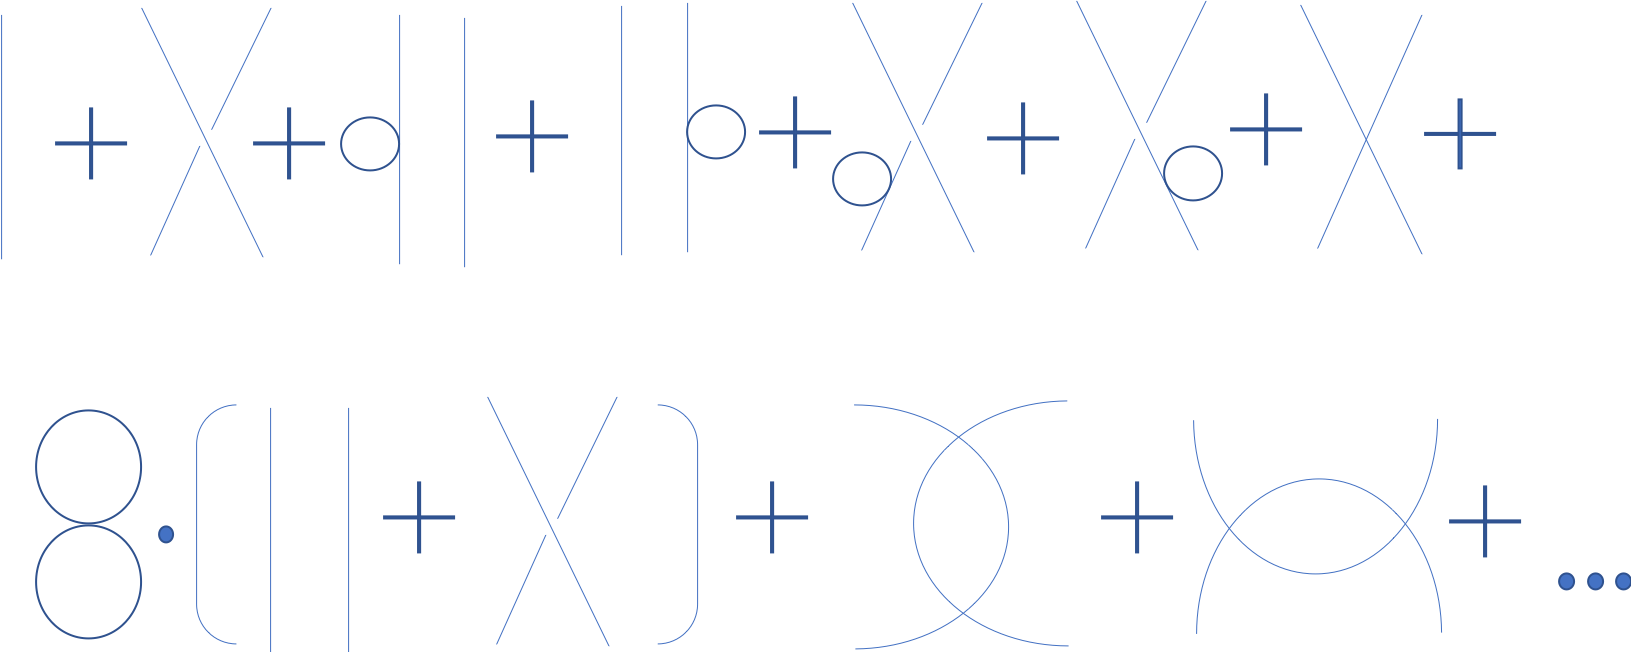
\includegraphics[width=4in]{images/phi4_diagrams.png}
\end{figure}

\noindent We can eliminate most of the infinite terms/diagrams by redefining the ground state energy $E_0$ and rest mass of the electron $m_0$ and rescaling $\lambda$, such that we dont have to set it to zero to make the theory work. \\

\noindent The first term/diagram that rescaling $\lambda$ does not work for introduces a logarithmic divergence and has the form

\begin{equation}
I = \frac{(-i \lambda)^2}{2} \int \frac{d^4 k}{(2 \pi)^4} \,\, \frac{i}{k^2 - m^2 + i \epsilon} \frac{i}{(k_1 + k_2 - k)^2 - m^2 + i \epsilon}.
\end{equation}

\noindent Therefore, we must impose a cutoff $|\Lambda| \ne \infty$ in order to calculate the $S$-matrix for $\phi^4$ theory. \\

\noindent Impose a cutoff on the momenta $|k| < k_c \in \mathbb{R}$. Then the integral above becomes (\textbf{Exercise})

\begin{figure}[H]
	\centering
	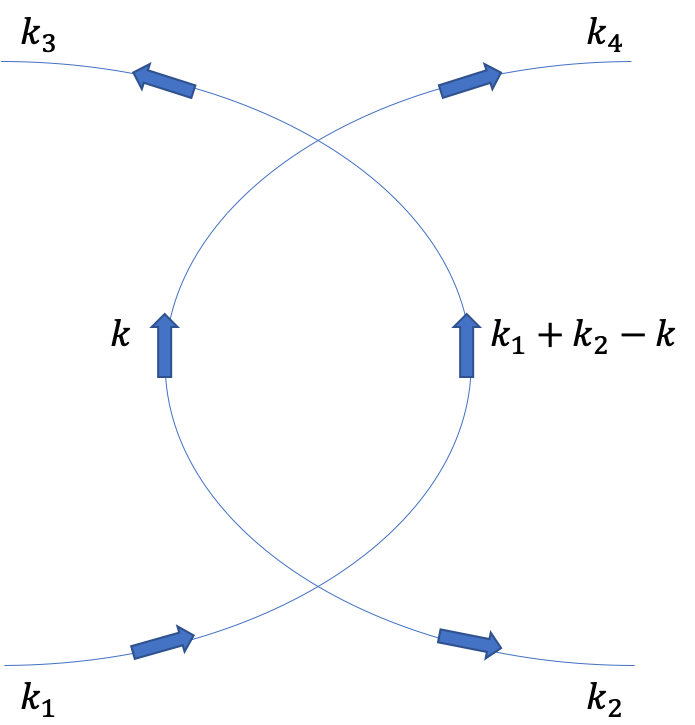
\includegraphics[width=1.5in]{images/cutoff_log.png}
\end{figure}

\begin{align}
I &= \frac{(-i \lambda)^2 i^2}{2} \int_\Lambda \frac{d^4 k}{(2 \pi)^4} \,\, \frac{i}{k^2 - m^2 + i \epsilon} \frac{i}{(k_1 + k_2 - k)^2 - m^2 + i \epsilon} \\
I &= 2 i C \log{\frac{k_c^2}{(k_1 + k_2)^2}}.
\end{align}

\noindent Then the scattering amplitude to order $\mathcal{O} (\lambda^2)$ is

\begin{equation}
\mathcal{M} = \mathcal{M} (k_c) = -i \lambda + i C \lambda^2 \left( \log{\left(\frac{k_c^2}{(k_1 + k_2)^2}\right)} + \log{\left(\frac{k_c^2}{(k_1 - k_3)^2}\right)} + \log{\left(\frac{k_c^2}{(k_1 - k_4)^2}\right)} \right).
\end{equation}

\noindent The parameter $z_2 = \lambda$ can be fit to the experiment and model, as we do not accept that it is fixed ``at the beginning of the Universe'', and we can declare victory by allowing $z_2 = z_2 (k_c) = \lambda (k_c)$. \\

\noindent To solve for $\lambda(k_c)$, let the scattering amplitude be the experimental value $\mathcal{M}(k_c, \lambda) = \mathcal{M}_{exp}$ and solve the differential equation that allows $\lambda$ to vary with respect to $k_c$ and match up to $\mathcal{M}_{exp}$

\begin{equation}
k_c \frac{d \lambda}{d k_c} = 6 C \lambda^2 + \mathcal{O} (\lambda^3).
\end{equation}

\clearpage

\section{Lecture 9: Renormalizability (of $\phi^4$ Theory)}
\label{sec: lec9}

\noindent This topic covers results of Bogoliubov, Parasiuk, Hepp, Zimmermann, or the BPHZ renormalization scheme. \\

\noindent A \textit{renormalizable} theory is a cutoff field theory determined by a finite number of parameters $\hat{H}_\Lambda = \hat{H} (z_1, \dots, z_n; \Lambda)$ such that for all observables $\hat{A}_\alpha$, the expectation value of $\hat{A}$ can be matched to experimentally determinable quantities for any choice of cutoff $\Lambda$ by redefining the parameters $z_j = z_j (\Lambda)$

\begin{equation}
\langle \hat{A}_\alpha \rangle _{z_1, \dots, z_n, \Lambda} = \langle \hat{A}_\alpha \rangle _{z_1 (\Lambda), \dots, z_n (\Lambda)} = \text{Experiment} (\alpha) .
\end{equation}

\noindent There is a weak form of renormailzability that retains dependence of the expectation value on the cutoff

\begin{equation}
\langle \hat{A}_\alpha \rangle _{z_1 (\Lambda), \dots, z_n (\Lambda)} = \text{Experiment} (\alpha) + \mathcal{O} \left(\frac{1}{k_c}\right).
\end{equation}

\noindent This dependence can be worked around, since as $k_c \rightarrow \infty$, the inverse goes to zero. \\

\noindent In the $\phi^4$ interaction, we have three parameters with the Hamiltonian

\begin{equation}
\hat{H} (m, \lambda, z ; \Lambda)
\end{equation}

\noindent Where $z$ is the field strength renormalization parameter. \\

\noindent Is $\phi^4$ theory, by this definition, renormalizable? \\

\noindent If this is true, then we are allowed to fit an infinite number of quantities to experimentally determinable quantities by fitting only three parameters: $m$, $\lambda$, and $z$. Very cool! \\

\subsection*{Degree of Divergence}

\noindent Consider a diagram with $B_E$ external lines. The diagram has a \textit{superficial degree of divergence} $D$ if it diverges with the cutoff as $k_c^D$. For $D=0$, we say that the diagram has logarithmic divergence: $\log{(k_c)}$. \\

\noindent \textbf{Theorem}: The degree of divergence is equal to the number of spacetime dimensions minus the number of external lines

\begin{equation}
D = 4 - B_E .
\end{equation}

\textbf{Examples}:

\begin{figure}[H]
	\centering
	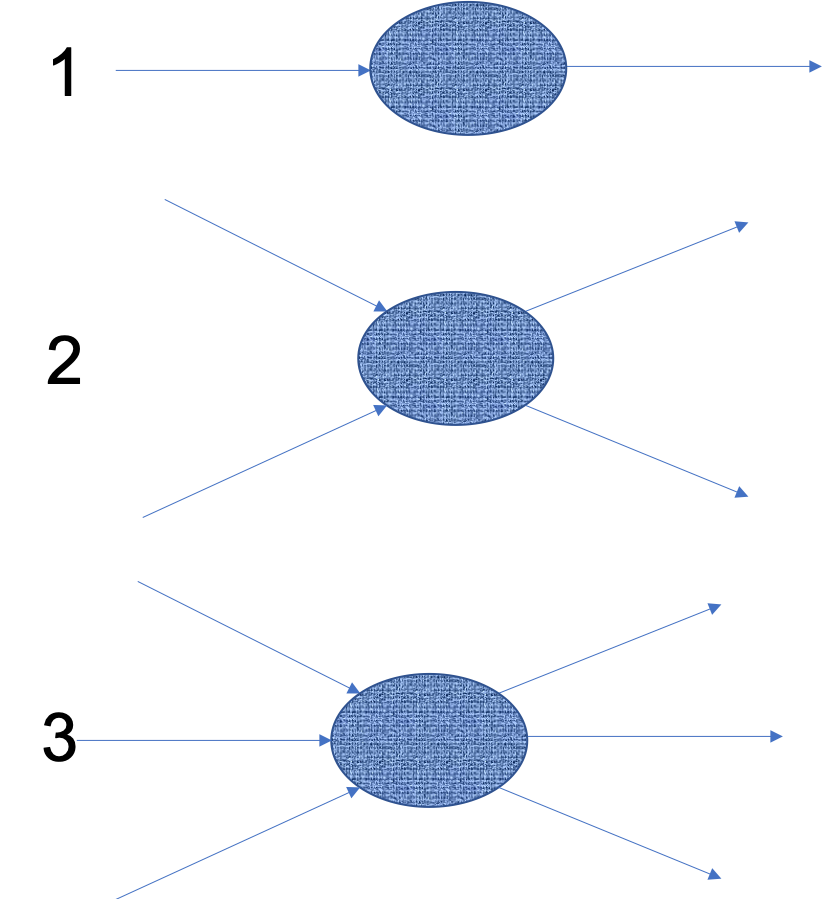
\includegraphics[width=2in]{images/dod_ex1.png}
\end{figure}

\begin{enumerate}
\item $B_E = 2 \implies D = 2 \implies \sim k_c^2$
\item $B_E = 4 \implies D = 0 \implies \sim \log{(k_c)}$
\item $B_E = 6 \implies D = -2 \implies \sim \frac{1}{k_c^2}$
\end{enumerate}

\noindent Note that as $B_E$ and $k_c$ increase, the divergences become increasingly less observable. Each pair of incoming/outgoing particles contributes a propagator proportional to $k_c^{-2}$ to the $4D$ momentum integral $\sim \,\, \int \frac{d^4 k}{(2 \pi)^4} \, \left(\frac{i}{k^2 - m^2 + i \epsilon}\right)^{\frac{B_E}{2}}$.  \\

\noindent Some more notation: $B_I$ is the number of internal lines, $V$ is the number of vertices, and $L$ is the number of closed loops. \\

\begin{figure}[H]
	\centering
	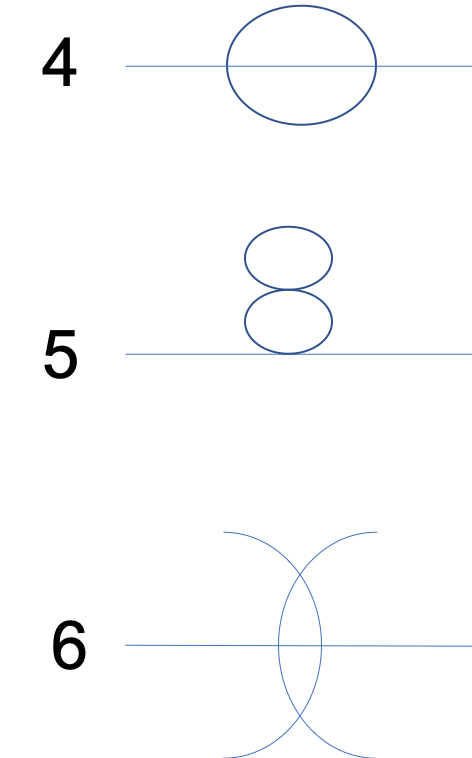
\includegraphics[width=1.5in]{images/dod_ex2.png}
\end{figure}

\begin{enumerate}
\item $B_I = 3$, $V=2$, $L=2$, $D=2$
\item $B_I = 3$, $V=2$, $L=2$, $D=2$
\item $B_I = 5$, $V=4$, $L=2$, $D=-2$
\end{enumerate}

\noindent \textbf{Proof}: \\

\noindent The number of loops corresponds directly to the number of undetermined momenta ($4D$ momentum space integrals). Morally, we say that $\int \frac{d^4 k}{(2 \pi)^4} \sim k_c^4$. \\
 
 \noindent It seems that there are $B_I$ such integrals, but momentum conservation reduces the total number of loop integrals to 
 
\begin{equation}
L = B_I - (V - 1).
\end{equation}

\noindent Each vertex has four lines and each line connects two vertices, such that 

\begin{equation}
4V = B_E + 2 B_I.
\end{equation}

\noindent Now, recall that for each loop there is a factor $\sim k_c^4$ from the integral, and for each line there is a factor $k_c^{-2}$ from the propagator. Then

\begin{equation}
D = 4 L - 2 B_I = 4 - B_E .
\end{equation}

\noindent \textbf{Exercise}: Prove this result for $n$-dimensional spacetime.

\subsection*{Physical or Renormalized Perturbation Theory}

\noindent Consider the parameterized Lagrangian

\begin{equation}
\mathcal{L} = \mathcal{L} (z_1 = m, z_2 = \lambda, z_3 = z) = \frac{1}{2} (z^2 (\partial_\mu \phi)^2 - z^2 m^2 \phi^2 ) - z^4 \frac{\lambda}{4!} \phi^4.
\end{equation}

\noindent Rewrite this in terms of the physical Lagrangian, the one that has been successful in corresponding with experimental data, and counter terms dependent on three new parameters $A$, $B$, and $C$,

\begin{align}
\mathcal{L} &= \mathcal{L}_{\text{phys}} + \text{counter terms} \\
\mathcal{L} &= \left(\frac{1}{2} (z^2 (\partial_\mu \phi)^2 - m_{\text{phys}}^2 \phi^2 ) - z^4 \frac{\lambda_{\text{phys}}}{4!} \phi^4 \right) + \left( A (\partial_\mu \phi )^2 + B \phi^2 + C \phi^4  \right)
\end{align}

\noindent Now, think of these parameters as additional interactions that can be shifted to eliminate the dependence on the cutoff. These parameters are determined iteratively by the constraint that physically observable quantities do not depend of the momenta $k$. \\

\noindent The Feynman rules for the renormalized $\phi^4$ theory are the same rules plus two more due to an additional type of vertex that depend of the ``additional interaction'' parameters.

\begin{figure}[H]
	\centering
	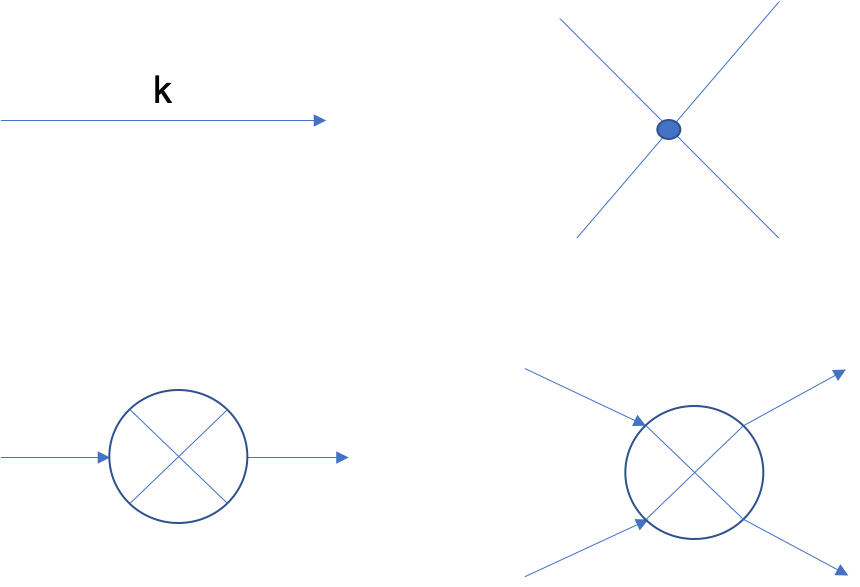
\includegraphics[width=3in]{images/renorm_feynman.png}
\end{figure}

$$
\begin{array}{lc}
\text{Top-left:} & \frac{i}{k^2 - m_{\text{phys}}^2 + i \epsilon} \\
\text{Top-right: }& -i \lambda_{\text{phys}} \\
\text{Bottom-left:} & 2 i (A k^2 + B) \\
\text{Bottom-right:} & 4! \cdot i C
\end{array}
$$

\noindent So, counter terms are added to the Lagrangian as ``additional interactions'', which introduce new Feynman diagrams. The parameters are determined iteratively to order $\lambda_{\text{phys}}^N$, at which we call them $A_N$, $B_N$, and $C_N$, and nothing depends on the cutoff. \\

\noindent The next iteration $N+1$ is determined by requiring that the new propagator (bottom-left diagram above) at $\lambda_{\text{phys}}^{N+1}$ has a pole at $m_{\text{phys}}$ with residue equal to one. We also require that the scattering amplitude to order $\mathcal{O} (\lambda_{\text{phys}}^{N+1})$ is equal to $-i \lambda_{\text{phys}}$ (bottom-right diagram above). \\

\subsection*{Non-Renormalizable Theories}

\noindent A non-renormalizable theory requires an infinite number of parameters to ensure that operationally-defined quantities do not depend on the cutoff. \\

\noindent How do these theories appear in renormalized perturbation theory? \\

\noindent For instance, consider the Lagrangian

\begin{equation}
\mathcal{L} = \mathcal{L}^0_{\text{phys}} + \mathcal{L}^{int}_{\text{phys}} (\lambda) + (\text{counter terms}) .
\end{equation}

\noindent Calculate the scattering amplitude to order $\mathcal{O} (\lambda_{\text{phys}}^{N})$, and we will see that we need counter terms to eliminate dependence on the cutoff $k_c$, but as we go to higher and higher order in $\lambda_{\text{phys}}$, we need more and more counter terms, and this will continue and diverge, requiring an infinite number of counter terms and associated parameters to eliminate the cutoff dependence.

\clearpage

\section{Lecture 10: Abelian Gauge Theory (Quantum Electrodynamics)}
\label{sec: lec10}


\noindent \textbf{Why study abelian gauge theory?}

\noindent An example of an abelian gauge theory is quantum electrodynamics and the electromagnetic field, as well as $SU(2)$, and $SU(3)$ gauge bosons. \\

\noindent In developing a gauge theory, we will follow the same route of specifying symmetries, giving rise to invariants, of the theory and then, via quantization, look for (projective) unitary representations of the group which are local. \\

\noindent As opposed to other field theories, the gauge theory should be symmetric under a local gauge group $\mathcal{G}$ which acts independently at each location in spacetime. \\

\noindent For example, consider the circle group $U(1)$, which consists of all complex numbers with absolute value equal to 1 under multiplication, the roots of unity

\begin{equation}
U(1) = \{ e^{i \theta} : \, \theta \in [0, 2 \pi ) \}.
\end{equation}

\noindent This symmetry group gives rise to the local gauge group $\mathcal{G}$ as the group of transformations from $1+3$-dimensional space time, Minkowski space, to the circle group

\begin{equation}
\mathcal{G} = \{ g: \,\, \mathcal{M}_{1+3} \rightarrow U(1) \}
\end{equation}

\noindent \textbf{How does the local gauge group act on fields? }\\

\noindent Consider the DIrac field, where we want a $U(1)$ gauge-invariant quantum field theory of electrons. Elements of $\mathcal{G}$ act independently on each spacetime location$x \in \mathcal{M}_{1+3}$. Equivalently, there is a copy of $U(1)$ attached to each $x$ acting independently of each other.

\begin{equation}
g: \, \psi (x) \rightarrow \pi ( g (x) ) \psi(x) = e^{i \alpha (x)} \psi (x)
\end{equation}

\noindent Where $\theta(x) \in [ 0 , 2 \pi )$ is a phase factor. \\

\noindent \textbf{Which theories are invariant under the Poincar\'e group and the local gauge group $\mathcal{G}$?} \\

\noindent As it stands, we have an empty set of theories that are invariant under the local gauge group. Begin populating it by building a Lagrangian density, with a classical, continuous spacetime, and find which kinds of terms will be invariant. \\

\noindent Terms of the Lagrangian density for the Dirac field that we already know to be invariant are $\bar{\psi}\psi$ and $(\bar{\psi} \gamma^/mu \psi)^2$ (contracted with itself). \\

\noindent Note that the quantity $\bar{\psi} \slashed{\partial} \psi$ is not invariant, as it is not well-defined!  Why? \\

\noindent The differential operator acting on the field $\partial_\mu \psi$ is a limit

\begin{equation}
\partial_\mu \psi \equiv \lim_{\epsilon \rightarrow \infty} \frac{ \psi(x + \epsilon n^\mu) - \psi(x)}{\epsilon}.
\end{equation}

\noindent And the local gauge group acting on this quantity results in oscillatory terms that do not converge as $\epsilon \rightarrow 0$ (e.g., $\sim e^{i\dots}$). The limit does exist under gauge transformations, since

\begin{equation}
g(\partial_\mu \psi) = \lim_{\epsilon \rightarrow \infty} \frac{1}{\epsilon} (e^{- \theta(x + \epsilon n^\mu)} \psi(x + \epsilon n^\mu ) - e^{i \theta(x)} \psi (x) ).
\end{equation}

\noindent This theory is boring at this moment, as the Lagrangian has only two gauge-invariant terms. To introduce dynamics and impose the desired symmetry, we need the derivative, but there is no way to do it with a single fermion (or boson) field. Therefore, we introduce an \textit{auxiliary field} which transforms nontrivially on the local gauge group (c.f., adding a catalyst in chemistry opens new thermodynamic paths for reactions to take place, as the catalyst is not consumed, but is used, in the reaction to lowers the free energy of the reaction). \\

\noindent Introduce the \textit{parallel transporter}, a recipe to compare a field at two independent spacetime locations, which is dependent on the path $\gamma$

\begin{equation}
U_\gamma (y,x) \in U(1), \,\, \forall \, x, y \in \mathcal{M}_{1+3}
\end{equation}

\noindent To ensure that $U(y,x)$ is a gauge invariant comparator, and allow us to compare the two spacetime locations in a gauge invariant, we require that the local gauage group act as

\begin{equation}
g: \,\, U(y,x) \rightarrow e^{i \alpha (y)} U(y,x) e^{-i \theta(x)}.
\end{equation}

\noindent So, we define $\psi(x)$ to be \textit{parallel transported} to $y$ as

\begin{align}
g: \,\, U(y,x) \psi(x) &\rightarrow e^{i \theta(y)} U(y,x) e^{-i \theta(x) }e^{- \alpha (x)} \psi(x) \\
&= e^{i \theta(y)} U(y,x)  \psi(x)
\end{align}

\noindent \textbf{Does such an object $U(y,x)$ exist?} \\

\noindent Yes, they exist and are made rigorous in the formalism of fibre bundles and principal bundles. Note that $U(y,x)$ is a not a field and is nonlocal object, but it is expressable in terms of local objects and local data. \\

\noindent So, $\psi(x + \epsilon n^\mu)$ and $U(x+\epsilon n^\mu, x)\psi(x)$ transform the same way under the local gauge group $\mathcal{G}$, and we can introduce dynamics to the theory and define the \textit{covariant derivative} as

\begin{equation}
D_\mu \psi (x) \equiv \lim_{\epsilon \rightarrow 0} \frac{\psi (x + \epsilon n^\mu) - U (x + \epsilon n^\mu, x) \psi (x)}{\epsilon}
\end{equation}

\noindent \textbf{What about the parallel transporter $U(y,x)$?} \\

\noindent Suppose that $U(x + \epsilon n^\mu , x)$ is continuous and differentiable near $x$, and apply the Taylor series expansion

\begin{align}
U(x + \epsilon n^\mu , x) &= U (x,x) + \epsilon n^\mu \partial_\mu U(x,x) + \dots \\
&= 1 + \epsilon n^\mu \partial_\mu U(x,x) +\dots \\
&= 1 - i \epsilon n^\mu A_\mu (x) + \dots
\end{align}

\noindent Where we tried $U(x,x)=1$, since $1$ transforms correctly under the gauge group, and it is traditional to call $\partial_\mu U(x,x) = -i \alpha A_\mu (x)$, where $\alpha$ is the fine structure constant. Now, $A_\mu (x)$ is not arbitrary, and must satisfy some constraints. \\

\noindent \textbf{How does $A_\mu (x)$ transform under $\mathcal{G}$?} \\

\noindent Apply a local gauge transformation $g \in \mathcal{G}$ to the last line above

\begin{equation}
e^{i \alpha (x + \epsilon n^\mu)} U(x + \epsilon n^\mu, x) e^{-i \theta(x)} = 1 - i \alpha \epsilon n^\mu A_\mu (x) + i n^\mu \partial_\mu \theta(x) + \dots
\end{equation}

\noindent Thus, the auxiliary field transforms under the local gauge as

\begin{equation}
g: \,\, A_\mu (x) \rightarrow A_\mu (x) - \frac{1}{\alpha} \partial_\mu \theta (x)
\end{equation}

\noindent And this gives us a definition of $A_\mu (x)$ in one gauge, and this transformation law allows us to change gauge, or basis. Finding the form of $A_\mu (x)$ that satisfies this local gauge transformation is tantamount to having an infinitesimal method for building the parallel transporter object. \\

\noindent Put this all together into the covariant derivative (\textbf{Exercise})

\begin{equation}
D_\mu \psi (x) = \partial_\mu \psi (x) + i \alpha A_\mu (x) \psi (x)
\end{equation}

\noindent Which is now a purely local object, dependent on only one spacetime location $x$. \\

\noindent Furthermore, the covariant derivative of the field transforms under the local gauge group by introducing the phase factor, the same as the action of $\mathcal{G}$ on the field $\psi$ itself

\begin{equation}
g: \,\, D_\mu \psi (x) \rightarrow e^{i \alpha (x)} D_\mu \psi (x)
\end{equation}

\noindent So, we've built the parallel transporter in terms of the local field $A_\mu (x)$, and we have a derivative object that transforms correctly under the local gauge group. Now, build the Lagrangian density

\begin{equation}
\mathcal{L} = \bar{\psi} \slashed{D} \psi - m \bar{\psi} \psi + \text{auxiliary field term(s)}
\end{equation}

\noindent To include the auxiliary field $A_\mu (x)$ in the quantization we need to endow it with dynamics. \\

\noindent \textbf{How do we give $A_\mu (x)$ dynamics?} \\

\noindent To first order,

\begin{equation}
U(x+\epsilon n^\mu , x) \sim e^{-i\alpha \epsilon n^\mu A_\mu (x + \frac{1}{2} \epsilon n^\mu)}.
\end{equation}

\noindent Use the parallel transporter to build a \textit{plaquette operator}, which transverses an object around a square of dimension $\epsilon$

\begin{figure}[H]
	\centering
	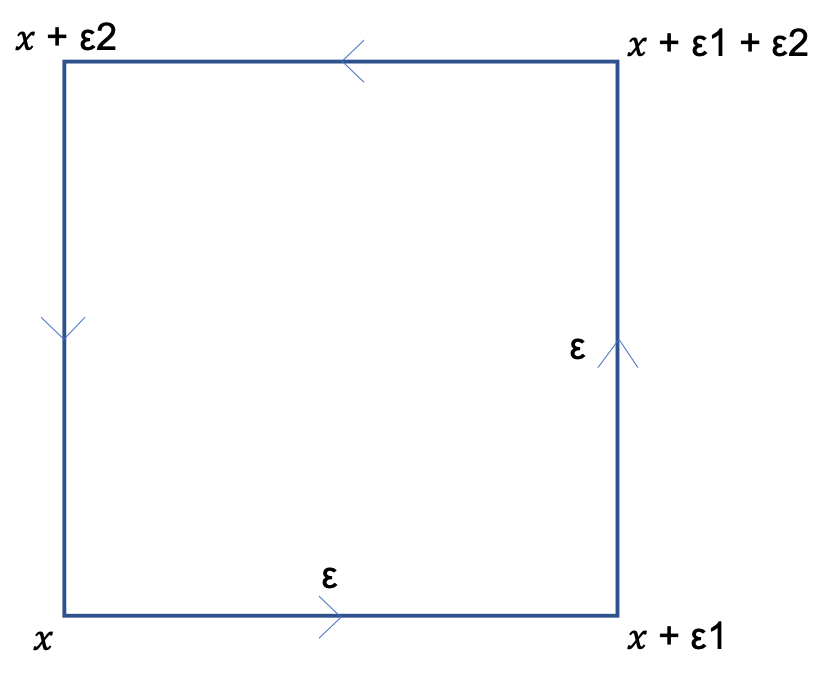
\includegraphics[width=2in]{images/plaquette.png}
\end{figure}

\begin{equation}
U_\Box(x)  = U(x, x + \epsilon \hat{1}) \cdot U (x + \epsilon \hat{1}, x + \epsilon (\hat{1} + \hat{2})) \cdot U(x + \epsilon (\hat{1} + \hat{2}), x + \epsilon \hat{2}) \cdot U(x + \epsilon \hat{2}, x).
\end{equation}

\noindent The plaquette operator $U_\Box$ is gauge invariant, and, working out the Taylor series, we can write it in terms of the auxiliary field (\textbf{Exercise})

\begin{equation}
U_\Box (x)  = e^{-i \epsilon \alpha (-A_2 (x + \frac{1}{2} \epsilon \hat{2}) - A_1 (x + \frac{1}{2} \epsilon \hat{1} + \epsilon \hat{2}) + A_2 (x + \epsilon \hat{1} +\frac{1}{2} \epsilon \hat{2}) + A_1 (x + \frac{1}{2} \epsilon \hat{1})) + \mathcal{O} (\epsilon^3)}.
\end{equation}

\noindent Expand in $\epsilon$ (\textbf{Exercise})

\begin{equation}
U_\Box (x) = 1 - i \epsilon^2 \alpha (\partial_1 A_2 - \partial_2 A_1 ) + \mathcal{O} (\epsilon^3).
\end{equation}

\noindent The choice of direction in this derivation is arbitrary, leaving 16 possible choices; construct the 2-tensor

\begin{equation}
F_{\mu\nu} (x) = \partial_\mu A_\nu - \partial_\nu A_\mu.
\end{equation}

\noindent Note that $F_{\mu\nu}$ is locally gauge invariant, Lorentz invariant, but it is not Poincar\'e invariant with those spacetime indices. Construct the gauge, Lorentz, and Poincar\'e invariant object from the $F_{\mu\nu}$

\begin{equation}
-\frac{1}{4} F^{\mu\nu} F_{\mu\nu}.
\end{equation}

\noindent Then the first nontrivial Langrangian density we can construct is the exact Lagrangian for quantum electrodynamics: an electromagnetic field minimally coupled to the Dirac field.

\begin{equation}
\mathcal{L} = \bar{\psi} (\slashed{D} - m) \psi -\frac{1}{4} F^{\mu\nu} F_{\mu\nu}.
\end{equation}

\noindent The term ``minimally coupled'' means that the theory is renormalizable. \\

\subsection*{Alternative Derivation of $F^{\mu\nu}$}

\noindent Since $D_\mu$ is gauage invariant, the commutator with itself $[D_\mu, D_\nu ]$ is also gauge invariant. So, under the local gauge group, the commutator transforms as

\begin{equation}
g: \,\, [D_\mu, D_\nu] \psi (x) \rightarrow e^{i \alpha (x)} [D_\mu, D_\nu] \psi (x).
\end{equation}

\noindent Plugging in the expression for the covariant derivative and working out the commutator, we get

\begin{equation}
[D_\mu, D_\nu] \psi (x) = [\partial_\mu, \partial_\nu] \psi + i \alpha ( [\partial_\mu, A_\nu] - [\partial_\nu, A_\mu]) \psi - \alpha^2 [A_\mu, A_\nu] \psi.
\end{equation}

\noindent The commutators of $\partial$ and $A$ with themselves are zero. Therefore,

\begin{equation}
[D_\mu, D_\nu] \psi (x) = i \alpha ( \partial_\mu A_\nu - \partial_\nu A_\mu) \psi (x)
\end{equation}

\noindent The commutator of the covariant derivative is the \textit{spacetime curvature tensor}.

\begin{equation}
[D_\mu, D_\nu] \psi (x) =i \alpha F_{\mu\nu} (x).
\end{equation}

\clearpage

\section{Lecture 11: Nonabelian Gauge Theory (Yang-Mills)}
\label{sec: lec11}


\noindent As a recap of abelian gauge theory, a \textit{gauge theory} is a theory that is invariant under a group $\mathcal{G}$ of local symmetry transformations, which act independently at each point in spacetime $\mathcal{M}_{1,3}$. \\

\noindent In contrast to local symmetry groups, a global symmetry group that we have dealt with extensively in the Poincar\'e group, which acts on all of spacetime, making such transformations dependent on spacetime location. \\

\noindent In the context of the Dirac spinor and fermionic field theories, consider the local phase transformation

\begin{equation}
\psi (x) \rightarrow e^{i \alpha (x)} \psi (x)
\end{equation}

\noindent Where we assumed that the phase function $\alpha (x)$, $x \in \mathcal{M}_{1,3}$, is differentiable, and maps Minkowski space to the radial unit interval, $\alpha (x): \, \mathcal{M}_{1,3} \rightarrow [0, 2 \pi )$. \\

\noindent The new, larger, more constrained symmetry group that we are building an invariant theory under is Poincar\'e group plus the local gauge group $\mathcal{G}$. The only terms invaraint under this new symmetry group that we found fit for the Lagrangian density were

\begin{equation}
\bar{\psi} \psi \text{ and } (\bar{\psi} \gamma^\mu \psi )^2.
\end{equation}

\noindent In order compare two independent points of spacetime in this theory, we introduced dynamics in the form of the covariant derivative. The covariant derivative was defined in terms of an auxiliary gauge field $A_\mu$

\begin{equation}
\partial_\mu \rightarrow \partial_\mu - i e A_\mu.
\end{equation}

\noindent Call $D_\mu = \partial_\mu - i e A_\mu$, and then we have the additional invariant term $\bar{\psi} \slashed{D} \psi$ to include in the Lagrangian density under this new representation of the derivative 

\begin{equation}
\mathcal{L} = \bar{\psi} \slashed{D} \psi + F^{\mu\nu} F_{\mu\nu}.
\end{equation}

\noindent Where $F^{\mu\nu}$ is the spacetime curvature tensor that includes derivatives of the gauge field $A_\mu$. \\

\subsection*{Nonabelian Gauge Theory}

\noindent Consider the gauge group to be the special unitary group of $2 \times 2$ matrices $SU(2)$. Note that for full generality, we should consider arbitrary connected Lie groups, but $SU(2)$ will get us almost all of the story, and the representation theory of $SU(2)$ groups can be used to find the representation theory of general Lie groups. \\

\noindent \textbf{What is the local gauge group of $SU(2)$?} \\

\noindent This theory must be invariant under group transformations $V(x) \in SU(2)$, where $x \in \mathcal{M}_{1,3}$. An element of this unitary group $V(x)$ has the following form and constraints

\begin{equation}
V(x) = \left(
\begin{array}{cc}
v_{00} (x) & v_{01} (x) \\
v_{10} (x) & v_{11} (x)
\end{array} \right)
\end{equation}

\begin{align*}
&\sum_{j,k=0}^1 |v_{jk}|^2 = 2 \\
& V^\dagger (x) V (x) = \mathbb{I} \\
& \text{det}(V(x)) = 1
\end{align*}

\noindent We need to choose how $V(x)$ acts on a field. Introduce two independent spinor fields $\psi_0 (x)$ and $\psi_1 (x)$ that form a new basis, under which the new theory must be invariant,

\begin{equation}
\psi_j (x) = \sum_{k=0}^1 v_{jk} (x) \psi_k (x).
\end{equation}

\noindent Build the doublet field as an $8 \times 1$ vector that Poincar\'e-transforms like two independent spinors

\begin{equation}
\Psi (x) = \left( \begin{array}{c} \psi_0 (x) \\ \psi_1 (x) \end{array} \right).
\end{equation}

\noindent \textbf{How does the local gauge group, with element $g \in \mathcal{G}$, act on the doublet field?} \\

\begin{equation}
g: \, \Psi (x) \rightarrow 
\left( \begin{array}{cc}
v_{00} (x) \cdot \mathbb{I}_{4 \times 4} & v_{01} (x) \cdot \mathbb{I}_{4 \times 4} \\
v_{10} (x) \cdot \mathbb{I}_{4 \times 4} & v_{11} (x) \cdot \mathbb{I}_{4 \times 4}
\end{array} \right)
\left( \begin{array}{c} \psi_0 (x) \\ \psi_1 (x) \end{array} \right).
\end{equation}

\noindent The invariant terms we can construct from the doublet field are 

\begin{equation}
\bar{\Psi} \Psi = \sum_{j=0}^1 \bar{\psi}_j \psi_j \text{ and } (\bar{\Psi} \Gamma^\mu \Psi)^2 \text{ , where } \Gamma^\mu = 
\left( \begin{array}{cc}
\gamma^\mu & 0 \\
0 & \gamma^\mu
\end{array} \right)
\end{equation}

\noindent As in the abelian case, build the covariant derivative by introducing the \textit{parallel transporter} $U(y,x) \in SU(2)$ and going to a representation of the local gauge group. Under the local gauge transformation

\begin{equation}
U(y,x) \rightarrow V(y) U(y,x) V^\dagger (x).
\end{equation}

\noindent The covariant derivative is then defined to be

\begin{equation}
n^\mu D_\mu \Psi \equiv \lim_{\epsilon \rightarrow 0} \frac{1}{\epsilon} (\Psi (x + \epsilon n) - U(x + \epsilon n, x) \Psi (x))
\end{equation}

\noindent Where we note that $U(x + \epsilon n, x)$ is a $2 \times 2$ matrix depending on two different spacetime locations. To ensure locality of the theory, we only need to know $U(y,x)$ for $y \simeq x$.\\

\noindent Stepping back, suppose that we have some element of the gauge group $U \in SU(2)$, which we assume is differentiable. Note that this $U$ is not the parallel transporter yet. \\

\noindent Since $U$ is unitary, and recalling that exponentiated unitary elements close to the identity are elements of the underlying Lie algebra, let

\begin{equation}
U = e^{i A}
\end{equation}

\noindent Where $A$ is a Hermitian matrix, such that $A^\dagger = A$ and $\text{Tr(A) = 0}$. \\

\noindent Though it is not necessary, we anticipate computation in the future, and choose a basis. Namely, we choose the $2 \times 2$ Pauli spin matrices as a basis, noting that any $2 \times 2$ Hermitian traceless matrix can be written as a combination of the three Pauli matrices. In the Pauli basis, the Hermitian matrix is

\begin{equation}
A = \sum_{j=1}^3 \frac{1}{2} \alpha^j \sigma^j.
\end{equation}

\noindent The Pauli matrices are

\begin{equation}
\sigma^1 = \frac{1}{2} \left( \begin{array}{cc}  0 & 1 \\ 1 & 0 \end{array} \right) 
\text{, } 
\sigma^2 = \frac{1}{2} \left( \begin{array}{cc} 0 & -i \\ i & 0 \end{array} \right) 
\text{, and } 
\sigma^3 = \frac{1}{2} \left( \begin{array}{cc}  1 & 0 \\ 0 & -1 \end{array} \right)
\end{equation}

\noindent And obey the Lie bracket

\begin{equation}
[ \sigma^j, \sigma^k] = i \epsilon^{jk}_{\,\,\,\,\,l} \sigma^l .
\end{equation}

\noindent So, to specify the Hermitian matrix $A$, we need three real numbers $\alpha^j \in \mathbb{R}$. \\

\noindent Consider some other Hermitian, traceless matrix $B$, which is to zeroth order equal to the identity, and to first order is proportional to the gauge field. Then the parallel transporter constructed from $B$ has the form

\begin{equation}
U(x + \epsilon n , x) = e^{i B(x;n,\epsilon)} = \mathbb{I}_{2\times 2} + \sum_{j=1}^3 i g \epsilon n^\mu A_\mu^j \frac{\sigma^j}{2} + \mathcal{O}(\epsilon^3)
\end{equation}

\noindent Then, in the chosen Pauli basis, the covariant derivative is an $8 \times 8$ matrix and is defined as

\begin{equation}
n^\mu D_\mu \Psi \equiv \lim_{\epsilon \rightarrow 0} \frac{1}{\epsilon} ( \Psi (x + \epsilon n) - U(x + \epsilon n, x) \Psi (x) )
\end{equation}

\noindent Where

\begin{equation}
D_\mu = \partial_\mu - i g A_\mu^j (x) \frac{\sigma^j}{2}.
\end{equation}

\noindent The coefficient field $A_\mu^j (x)$ is not arbitrary and must obey transformation laws of the local gauge group, as well as give a representation of the local gauge group determined by the action of the local gauge group on the parallel transporter

\begin{align}
V: \, U(x + \epsilon n, x) \rightarrow& V(x + \epsilon n) U(x + \epsilon n, x) V^\dagger (x) \\
&= V(x + \epsilon n) \left( \mathbb{I} + i g \epsilon n^\mu A_\mu^j \frac{\sigma^j}{2} + \mathcal{O} (\epsilon^3) \right) V^\dagger (x)
\end{align}

\noindent Calculating the action of  $V(x + \epsilon n)$ and $V^\dagger (x)$, the first order term in $\epsilon$ becomes (\textbf{Exercise})

\begin{equation}
\text{L.G.}: \, A_\mu^j (x) \frac{\sigma^j}{2} \rightarrow V(x) \left( A_\mu^j \frac{\sigma^j}{2} + \frac{i}{2} \partial_\mu \right) V^\dagger (x) .
\end{equation}

\textbf{Hint:} $V(x+\epsilon n) V^\dagger (x) = \left[ (1+\epsilon n^\mu \partial_\mu)V(x) \right] V^\dagger (x) + \mathcal{O}(\epsilon^2)$. \\

\noindent Next, to compute $V(x) \partial_\mu V^\dagger (x)$, we will take the infinitesimal approach. Recall that for the abelian case, we just had the phase factor $\alpha(x) \partial_\mu \alpha^\dagger (x)$, which was just a number, but now with $V(x)$ we have a $2 \times 2$ matrix with an $8 \times 8$ representation. \\

\noindent When $V(x)$ is infinitesimally close to the identity, we know that it is some exponential factor in the Pauli sigma matrices

\begin{equation}
V(x) = e^{i \alpha^j (x) \frac{\sigma^j}{2}}
\end{equation}

\noindent Where $\alpha^j (x)$ are small numbers. Applying the Taylor expansion with respect to $\alpha(x)$, the action of $V(x)$ on the partial derivative is

\begin{align}
V(x) \partial_\mu V^\dagger (x) &= (\mathbb{I} + i \alpha^j \frac{\sigma^j}{2}) \partial_\mu (\mathbb{I} - i \alpha^j \frac{\sigma^j}{2}) \\
&= -i \frac{\partial \alpha^j}{\partial x^\mu} \frac{\sigma^j}{2} + \mathcal{O}(\alpha^2)
\end{align}

\noindent Then, under the local gauge transformation, the gauge field and sigma matrices transform as

\begin{equation}
\text{L.G.}: A_\mu^j (x) \frac{\sigma^j}{2} \rightarrow A_\mu^j (x) \frac{\sigma^j}{2} + \frac{1}{g} (\partial_\mu \alpha^j (x)) \frac{\sigma^j}{2} + i \left[ \alpha^j (x) \frac{\sigma^j}{2}, A_\mu^k (x) \frac{\sigma^k}{2} \right].
\end{equation}

\noindent Now we can see the infinitesimal local gauge transformation does to the covariant derivative of the doublet spinor field $\Psi (x)$

\begin{align}
&\text{L.G.}: \Psi (x) \rightarrow \left( \mathbb{I} + i \alpha^j (x) \frac{\sigma^j}{2} \right) \Psi (x) \\
&\text{L.G.}: D_\mu \Psi (x) \rightarrow \left( \partial_\mu - i g A_\mu^j (x) \frac{\sigma^j}{2} - i (\partial_\mu \alpha^j (x)) \frac{\sigma^j}{2} + g \left[ \alpha^j (x) \frac{\sigma^j}{2}, A_\mu^k (x) \frac{\sigma^k}{2} \right] \right) \left(1 + i \alpha^j (x) \frac{\sigma^j}{2} \right) \Psi (x)
\end{align}

\noindent To first order in $\alpha$, the right-hand side of the infinitesimal transformation becomes

\begin{align}
\text{L.G.}: D_\mu \Psi (x) &\rightarrow \left( 1 + i \alpha^j (x) \frac{\sigma^j}{2} \right) D_\mu \Psi (x) \\
&= V(x) D_\mu \Psi (x)
\end{align}

\noindent Where, for the physicist, ignoring issues of connectivity with the local gauge group (will need \textit{gauge fixing}), we make the ``big'' gauge transformation (last line) by exponentiating (e.g., $(1+\frac{x}{n})^n = e^x$). \\

\noindent Now we need to build a Langrangian density term that gives dynamics to the gauge field $A^j_\mu (x)$. Recall the commutator $[D_\mu, D_\nu]$, the curvature of the $SU(2)$ fibre bundle, which is local gauge invariant, and involves derivatives of $A_\mu^j$. This transforms under local gauge as

\begin{equation}
\text{L.G.}: [D_\mu, D_\nu] \Psi (x) \rightarrow V(x) [D_\mu, D_\nu] \Psi (x).
\end{equation}

\noindent In the nonabelian case, the commutator has the form, using the fact that mixed partial derivatives commute (\textbf{Exercise})

\begin{align}
[ D_\mu, D_\nu] &= i g F_{\mu\nu}^{\,\,\,\,j} \frac{\sigma^j}{2} \\
&= ig \left( \partial_\mu A_\nu^j \frac{\sigma^j}{2} - \partial_\nu A_\mu^j \frac{\sigma^j}{2} - i g \left[ A_\mu^j \frac{\sigma^j}{2}, A_\nu^k \frac{\sigma^k}{2} \right] \right)
\end{align}

\noindent So, in the nonabelian case, the curvature tensor $F_{\mu\nu}$ depends quadratically on $A_\mu^j$, whereas in the abelian case it was linearly dependent. Therefore, the invariant term $\sim F^{\mu\nu}F_{\mu\nu}$ yields cubic and quartic terms in the Lagrangian density, making an ``interacting'' theory. \\

\noindent Under the local gauge, the curvature tensor transforms as similarity

\begin{equation}
\text{L.G.}: F_{\mu\nu}^{\,\,\,\,j} \frac{\sigma^j}{2} \rightarrow V(x) (F_{\mu\nu}^{\,\,\,\,j}) V^\dagger (x).
\end{equation}

\noindent By the similarity transformation, we can build an invariant Lorentz scalar with the trace of the invariant term (\textbf{Exercise, Check}, $\sigma^j \sigma^k$ introduces $\delta_{jk}$)

\begin{equation}
\text{Tr}\left( \left( F_{\mu\nu}^{\,\,\,\,j} \frac{\sigma^j}{2} \right)\left( F_{\mu\nu}^{\,\,\,\,k} \frac{\sigma^k}{2} \right) \right)= \frac{1}{8} (F_{\mu\nu}^{\,\,\,\,j})^2.
\end{equation}

\noindent The (classical) Langrangian density for the nonabelian gauge theory, invariant under local gauge and Poincar\'e transformations is

\begin{equation}
\mathcal{L} = \bar{\Psi} (i \slashed{D} - m) \Psi - \frac{1}{4} (F_{\mu\nu}^{\,\,\,\,j})^2.
\end{equation}

\noindent This can be quantized in two ways:

\begin{enumerate}
\item Perturbatively via path integrals
\item Non-perturbatively via lattice discretization.
\end{enumerate}

\noindent Note that in the abelian case (theory of QED), the dynamics in the Lagrangian density of the gauge field were quadratic, essentially resulting in the wave equation. In the nonabelian case, they are quartic.


\clearpage

\section{Lecture 12: Quantization of Gauge Theories}
\label{sec: lec12}


\noindent Recall the classical Lagrangian density $\mathcal{L} = \bar{\psi}(i \slashed{D} - m) \psi - \frac{1}{4} F_{\mu\nu}^{\,\,\,\,a} F^{\mu\nu, \, a}$, where $a$ denotes individual fields, that we crafted to be invariant under the local gauge symmetry group $SU(2)$. We introduced the ``helper'' gauge field $A_{\mu}^a$ which manifests in the terms of the spacetime curvature tensor , or the curvature of the $SU(2)$ fibre bundle, $F_{\mu\nu} = -i [D_\mu, D_\nu]$, where $D_\mu = \partial_\mu - i g A_\mu^a \frac{\sigma^a}{2}$ is the covariant derivative. \\

\noindent This Langrangian density represents a nontrivial dynamical system that is invariant under the local gauge symmetry group and endows fermions, as well as other fields, with dynamics. Unlike many other effective classical theories, this one is not quadratic in its fields and yields nonlinear equations of motion (e.g., instanton and soliton solutions). \\

\noindent We now quantize this gauge theoryto build a quantum theory that is invariant under the Poincar\'e and local gauge symmetry groups by finding the correct representation that has this Lagrangian density as its effective classical limit. \\

\noindent Two problems that arise for the gauge theories are (1) the classical theory ($\mathcal{L}_0$) is already nonlinear, and (2) there are lots of symmetries, global and local. Local symmetries are represented by copies of $SU(2)$ acting independently of each other at each spacetime location. \\

\noindent Two approaches of quantization that we will explore include (1) an analytic, but naive \textit{path integral quantization} $\int \mathcal{D} A \mathcal{D} \psi \mathcal{D} \bar{\psi} e^{i S}$ that is good for high-energy scattering processes, but not for calculating ground state correlation functions. The mathematical rigor of this approach is a current topic of research. And (2) a computational route of \textit{lattice quantization}, which makes dealing with nonlinearity ``easy'', but it loses Poincar\'e invariance in the process. Note that there is also the route of canonical quantization, but we will not bother with that here.

\subsection*{Path Integral Quantization of Gauge Theories}

\noindent First, some words on the space of all gauge fields $A_\mu^a$: note that $A_\mu^a \frac{\sigma^a}{2}$ and $A_\mu^a \frac{\sigma^a}{2} + \frac{1}{g} (\partial_\mu \alpha^a) \frac{\sigma^a}{2} + i [\alpha^b \frac{\sigma^b}{2}, \alpha^c \frac{\sigma^c}{2}]$ are \textit{gauge equivalent}, meaning that there exists an infinite number of $A_\mu^a$'s with the same path integrand $e^{i S}$, causing the path integral to result in infinity, since we are redundantly integrating over a continuous infinity of physically equivalent field configurations. \\

\noindent Consider the gauge field $A_\mu^a$, a list of 12 numbers in $(3+1)$-dimensional spacetime, on $(0+1)$-dimensional spacetime $\mathcal{M}_{0+1}$ (e.g., a line), where $A_\mu^a$ is still a list of three numbers. Now, $SU(2)$ acts independently on $A_\mu^a$ at each point in $\mathcal{M}_{0+1}$. This action is tantamount to multiplying by a phase on a sphere $S^3$ at each spacetime location, since $SU(2)$ is parameterized by four numbers, the coefficients of the quaternions with norm equal to one. Below is a schematic of the space of all $A_\mu^a$'s. \\

\begin{figure}[H]
	\centering
	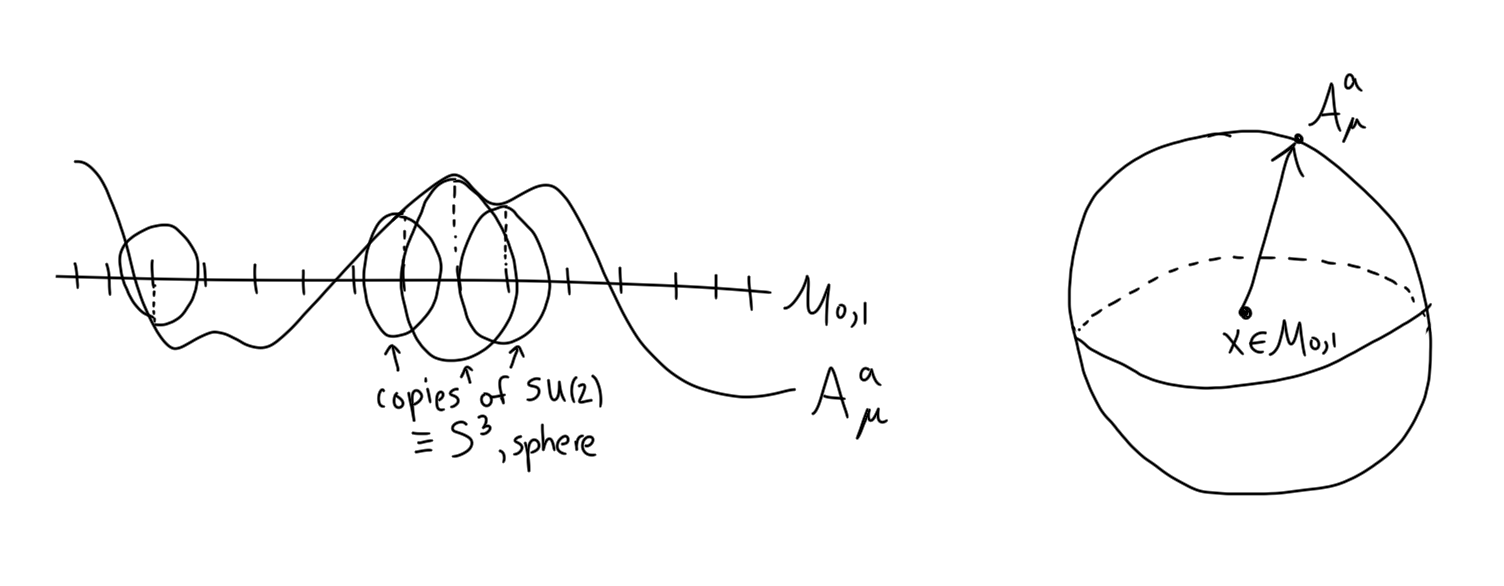
\includegraphics[width=4in]{images/su2schematic.png}
	\caption*{Schematic of gauge field configurations, independent copies of $SU(2)$ acting on $(0+1)$-dimensional spacetime.}
\end{figure}

\noindent So $A_\mu^a$ is like a vector on $S^3$ at each spacetime location and is a possible configuration in $\mathcal{M}_{0+1}$. These configurations form an equivalence class  $[A_\mu^a]$ defined by the local gauge group $\mathcal{G}$. Addressing the problem of very many symmetries, global and local,  in the path integral approach, there are very many equivalence classes, or configurations, to sum over, but we'd like to just choose one configuration. \\

\noindent Another, more common schematic to demonstrate the action of gauge groups is to consider rotations in $SO(2)$, where our theory is a zero-dimensional theory invariant under $SO(2)$. Configurations in this schematic are just points in a two-dimensional space with equivalence classes defined by circles centered at the origin. See schematic below. \\

\begin{figure}[H]
	\centering
	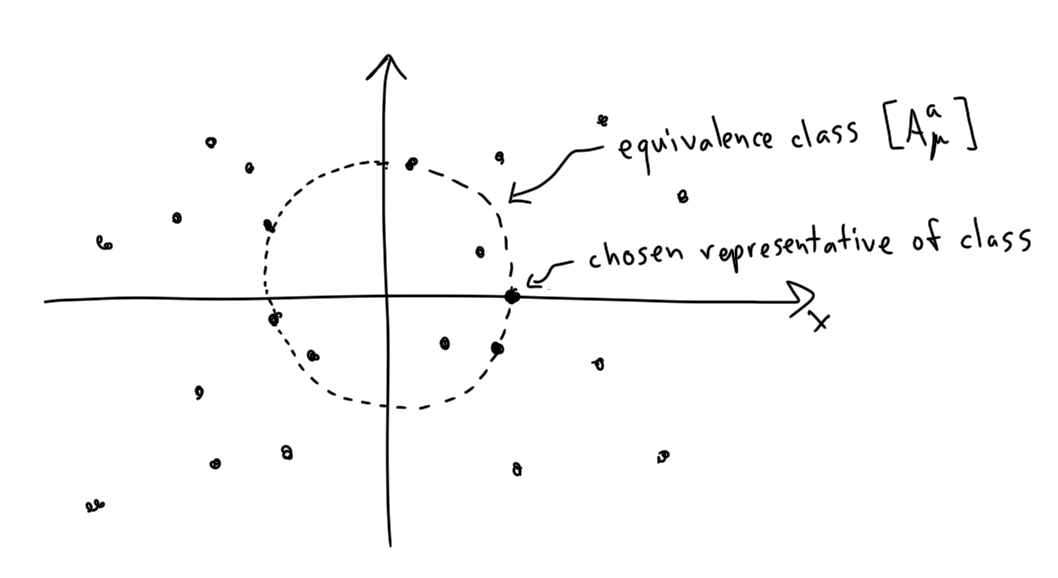
\includegraphics[width=4in]{images/so2schematic.png}
	\caption*{Schematic of gauge field configurations and equivalence classes represented by rotations in $SO(2)$.}
\end{figure}

\noindent In choosing a representative point per equivalence class, we enforce the \textit{gauge fixing condition}. A good choice of representative may be the point that crosses the horizontal axis. We then integrate over the space of the chosen representatives. This effectively reduces the size of the configuration space and makes the path integral much more tractable. \\

\noindent Note that we only pick one representative per equivalence class, but there can be more than one depending on the choice of gauge fixing condition, where the gauge fixing condition if a function that crosses the equivalence class circle more than once. This is called the \textit{Gribov ambiguity}, and commonly happens in the Coulomb gauge. \\

\begin{figure}[H]
	\centering
	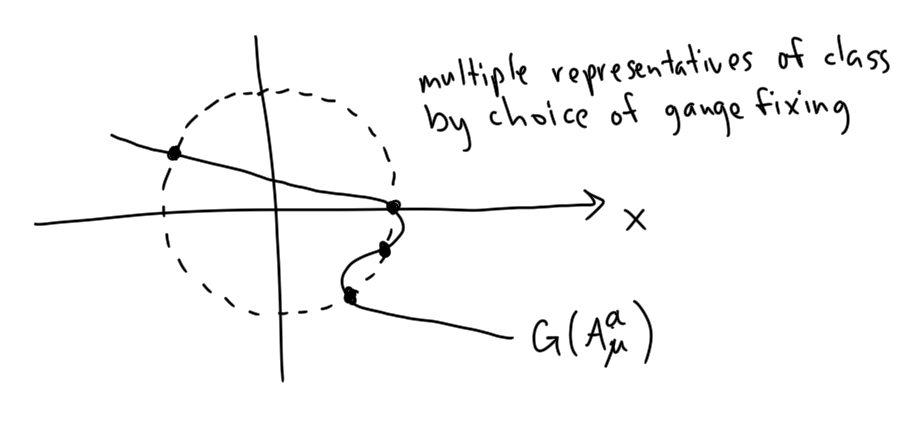
\includegraphics[width=3in]{images/gribov.png}
	\caption*{Example schematic of Gribov ambiguity, where more than one representative of the equialvence class is chosen by the guage fixing condition.}
\end{figure}

\subsubsection*{Gauge Fixing Condition}

\noindent Recall that the path integral approach is made difficult by the fact that we are redundantly integrating over a continuous infinity of physically equivalent field configurations. By applying a gauge fixing condition, we isolate the intersting part of the integral and count each distinct physical configuration only once. Finding the right gauge fixing function $G$ allows us to separate out this overcounting in the path integral and throw it away. Note that we are free to ``throw it away'' since we are \textit{guessing} a quantum theory.\\

\noindent Choosing the gauge fixing function to be $G(A_\mu^a) = \partial_\mu A_\mu^a - \omega^a$, where $\omega^a$ is any scalar field, is a generalization of the Lorentz gauge, and setting this equal to zero is a generalization of the Lorentz gauge condition

\begin{equation}
G(A_\mu^a) = \partial_\mu A_\mu^a - \omega^a = 0.
\end{equation}

\noindent With the gauge fixing function, the way we separate the overcounting is by inserting unity

\begin{equation}
1 = \int \mathcal{D} \alpha \,\, \delta(G(A^\alpha)) \, \text{det} \left( \frac{\delta G(A^\alpha)}{\delta \alpha} \right).
\end{equation}

\noindent Breaking equation this down, we are performing a path integral over all possible gauge transformations, and picking out only the $G(A^\alpha)$ that equals zero, obeying the gauge fixing condition, choosing a single representative of the equivalence class. The determinant is called the \textit{Faddeev-Popov determinant}. The notation $A^\alpha$ indicates the locally gauge transformed gauge field

\begin{align}
(A^\alpha)^a_\mu &= A^a_\mu + \frac{1}{2} \partial_\mu \alpha^a + f^{abc} A_\mu^b \alpha^c \\
&= A_\mu^a + \frac{1}{g} D_\mu \alpha^a
\end{align}

\noindent Where $f^{abc}$ are the structure constants from the Pauli spin matrix commutation relations

\begin{equation}
\left[ \frac{\sigma^a}{2}, \frac{\sigma^b}{2} \right] = i f^{abc} \frac{\sigma^c}{2}.
\end{equation}

\noindent This way of writing 1 is the continuous, functional generalization of that for discrete, many-variable $n$-dimensional vectors

\begin{equation}
1 = \left( \prod_{j=1}^n \int d a_j \right) \delta^{(n)} (\textbf{g}(\textbf{a})) \text{det} \left( \frac{\partial g_j}{\partial a_k} \right)
\end{equation}

\noindent Where the determinant here is the Jacobian of the change of variables. By change of variables, this can be written as (\textbf{Exercise})

\begin{equation}
1 = \left( \prod_{j=1}^n \int d b_j \right) \delta^{(n)} (\textbf{b}).
\end{equation}

\noindent Inserting the contiuous, functional version of one into the path integral, we now have an expression that integrates over the equivalence classes but ``sucks out'' the overcounting to just one representative of the class

\begin{equation}
\int \mathcal{D} \alpha \int \mathcal{D} A \mathcal{D} \psi \mathcal{D} \bar{\psi} \,\, \delta(G(A^\alpha)) \text{det} \left( \frac{\delta G(A^\alpha)}{\delta \alpha} \right) e^{i S}.
\end{equation}

\noindent Evaluating the Faddeev-Popov determinant in our choice of the Lorentz gauge (\textbf{Exercise})

\begin{align}
\text{det} \left( \frac{\delta G(A^\alpha)}{\delta \alpha} \right) &= \text{det} \left( \frac{1}{g} \partial^\mu D_\mu \right) \\
&= \int \mathcal{D} c \mathcal{D} \bar{c} \,\, e^{i \frac{1}{g} \int d^4 x \, \bar{c} (-\partial^\mu D_\mu) c}
\end{align}

\noindent Where, recall from the study of fermions, we have used auxiliary Grassman-valued, scalar, spin-0 fields $c$ and $\bar{c}$. These fields are non-physical and must disappear form the final results: \textit{Faddeev-Popov ghosts} or \textit{ghosts}. \\

\noindent Inserting the ghost expression for the determinant into the path integral, we now have

\begin{align}
\int \mathcal{D} \alpha \int \mathcal{D} A \int \mathcal{D} c \mathcal{D} \bar{c} \int \mathcal{D} \psi \mathcal{D} \bar{\psi} \,\, \delta( \partial^\mu A^a_\mu - \omega^a ) e^{i (S + \frac{1}{g} \int d^4 x \, \bar{c} (-\partial^\mu D_\mu) c)}.
\end{align}

\noindent Integrate out the delta functional, since $\omega^a$ is arbitrary, using an Gaussian integral over $\omega^a$ with coefficient $\xi \in [0,1]$, and calling $S' = S + \frac{1}{g} \int d^4 x \, \bar{c} (-\partial^\mu D_\mu) c$,

\begin{equation}
\int \mathcal{D} \omega \, e^{-i \int d^4 x \, \frac{1}{2} \xi (\omega^a)^2} \left( \int \mathcal{D} ... \right) \delta( \partial^\mu A_\mu^a - \omega^a) e^{i S'}
\end{equation}

\noindent Since $\omega^a$ is an arbitrary, gauge-fixing, scalar function that takes one representative of each independent equivalence class, the full path integral will now be independent of $\omega^a$, and we have the form

\begin{equation}
N(\xi) \int \mathcal{D} \alpha \int \mathcal{D} A \int \mathcal{D} c \mathcal{D} \bar{c} \int \mathcal{D} \psi \mathcal{D} \bar{\psi} \,\,  e^{i \int d^4 x \, \mathcal{L}'} .
\end{equation}

\noindent The Lagrangian $\mathcal{L}'$ has the form

\begin{equation}
\mathcal{L}' = \bar{\psi} (i \slashed{D} - m) \psi - \frac{1}{4} (F^a_{\mu\nu})^2 + \frac{1}{2} \xi (\partial^\mu A_\mu^a)^2 + \frac{1}{g} \bar{c}^a (-\partial^\mu D_\mu^{ab}) c^b.
\end{equation}

\noindent Note that the integral over $\alpha$ blows up to infinity, but in correlation functions we always have ratios of the path integrals and the $N(\xi) \cdot \infty$'s will cancel out. \\

\noindent Remaining questions include

\begin{itemize}
\item Does the path integral above even define a quantum theory, and is it invariant under Poincar\'e and local gauge symmetry group transformations? 
	\subitem See the work of `t Hooft.
\item Do the ghosts $c$ and $\bar{c}$ vanish from the processes? 
	\subitem Feynman diagrams will clear up this concern.
\item Is the Lagrangian density (theory) $\mathcal{L}'$ renormalizable?
	\subitem Also see the work of `t Hooft.
\end{itemize}


\clearpage

\section{Lecture 13: Quantization of Nonabelian Gauge Theory}
\label{sec: lec13}


\noindent In the path integral quantization of gauge theories, we started by guessing a quantum theory by integrating the action functional over fermion fields $\psi$, $\bar{\psi}$ and gauge boson fields $A$ to calculate transition amplitudes. \\

\noindent We noticed that there are many gauge-equivalent configurations of the gauge field that causes naive divergences, due to overcounting, in the Feynman diagram expansion. To tame this infinity, we fixed the gauge by choosing a single representative from each gauge equivalence class by inserting unity in terms of the delta functional. This introduced a nonlinear Jacobian term  $\text{det} \left( \frac{\delta G(A^\alpha)}{\delta \alpha} \right)$, where $A^\alpha$ denotes the gauge-fixed gauge field. \\

\noindent To compute this determinant, we introduced the auxiliary (classical, scalar, spinless) Grassman-valued fields $c(x)$, called Faddeev-Popov ghosts. These fields are unphysical, and must drop out during calculation. Note that the PCT-thereom does not apply to ghosts. Then transition amplitude is then defined as

\begin{equation}
\bra{\Phi_f} U \ket{\Phi_i} \equiv \int \mathcal{D} A \mathcal{D} \psi \mathcal{D} \bar{\psi} \mathcal{D} c \mathcal{D} \bar{c} \,\, e^{i S}.
\end{equation}

\noindent Where the ghosts obey the anticommutation relation as Grassman-valued fields $\{c(x), c(y)\} = 0$, and the Lagrangian density is

\begin{equation}
\mathcal{L} = -\frac{1}{4} (\partial_\mu A_\nu^a - \partial_\nu A_\mu^a)^2 + \frac{1}{2} \xi (\partial^\mu A_\mu^a)^2 + \bar{\psi} (i \slashed{\partial} - m) \psi + \bar{c}^a (-\partial^\mu \partial_\mu ) c^a + \mathcal{L}_{int} (g) .
\end{equation}

\noindent Note that the interacting bits, including the bits from the covariant derivative $D_\mu$ are absorbed into $\mathcal{L}_{int} (g)$, and everything else in the expression above is the free theory with partial derivatives $\partial_\mu$. \\

\noindent We now push forward under the belief that the perturbatively defined theory above is representative of a quantum theory, and expand in powers of the interaction term $g$ to define processes and Feynman rules of the \textbf{Yang-Mills theory}.

\subsection*{Propagators (free theory, $g=0$ part)}

\noindent The fermion propagator contributes 

\begin{equation}
\langle \bar{\psi}_{j \alpha} (x) \hat{\bar{\psi}}_{l \beta} (y) \rangle = \int \frac{d^4 k}{(2 \pi)^4} \, \left( \frac{i}{\slashed{k} - m} \right)_{\alpha \beta} \delta_{jl} e^{-i k \cdot (x-y)}.
\end{equation}

\noindent The gauge boson propagator contributes 

\begin{equation}
\langle \hat{A}_\mu^a (x) \hat{A}_\nu^b (y) \rangle = \int \frac{d^4 k}{(2 \pi)^4} \,\, \left( \eta_{\mu\nu} - (1-\xi) \frac{k_\mu k_\nu}{k^2} \right) \delta_{ab} \frac{e^{-i k \cdot (x-y)}}{k^2 + i \epsilon}.
\end{equation}

\noindent The ghost propagator contributes 

\begin{equation}
\langle \hat{c}^a (x) \hat{\bar{c}}^b (y) \rangle = \int \frac{d^4 k}{(2 \pi)^4} \,\, \frac{i}{k^2} \delta_{ab} e^{-i k \cdot (x-y)}.
\end{equation}

\noindent Recall that $a$, $b = 1,2,3$ and $\mu$, $\nu = 0,1,2,3$.

\subsection*{Vertices (interacting theory, $g \ne 0$ part)}

\noindent The interaction of two fermions and one gauge boson contributes

\begin{equation}
i g \gamma^\mu \frac{\sigma^a}{2}.
\end{equation}

\noindent The interaction of three gauge bosons contributes

\begin{equation}
g f^{abc} \left( \eta^{\mu\nu}(k-p)^\rho + \eta^{\mu\rho} (p-q)^\mu + \eta^{\rho\mu} (q-k)^\nu \right).
\end{equation}

\noindent The interaction of four gauge bosons contributes

\begin{equation}
-ig ( f^{abc} f^{cde} (\eta^{\mu\rho} \eta^{\nu\sigma} - \eta^{\mu\sigma} \eta^{\nu\rho}) + f^{ace} f^{bde} (\eta^{\mu\nu} \eta^{\rho\sigma} - \eta^{\mu\sigma} \eta^{\nu\rho}) + f^{ade} f^{bce} (\eta^{\mu\nu} \eta^{\rho\sigma} - \eta^{\mu\rho} \eta^{\nu\sigma}) ).
\end{equation}

\noindent The interaction of one gauge boson with two ghosts contributes

\begin{equation}
g f^{abc} p^\mu.
\end{equation}

\noindent (\textbf{Exercise}) And the rest of the Feynman rules for Yang-Mills theory: symmetry factors, signs, and conservations laws.  \\

\subsubsection*{Big Question 1}

\noindent Can we interpret this as a quantum theory? In other words, does this theory implicitly define the Hermitian operators $\hat{A}^\alpha$, $\hat{\psi}$, and $\hat{c}$? \\

\noindent \textbf{Yes}, it is a quantum theory, subject to a cutoff. \\

\noindent In more detail, what are the possible modes of failure for the theory to not be a valid quantum theory? \\

\noindent The first mode of failure that can occur is the time evolution operator not being unitary, or time translation not being a unitary process. To confirm that time translation in this theory is a unitary process, check that the correlation function is symmetric under the group of Poincar\'e transformation (\textbf{Exercise}). This also implies that probability is conserved. \\

\noindent The second mode of failure occurs if, after building the Fock space, we get negative norm states, such that the inner product of the system eigenstates is less than zero $\braket{\Psi | \Psi} < 0$. If this happens, then the Hamiltonian is not positive definite and we do not have a proper Hilbert space. \\

\noindent Note that there is a type of exception to this rule, which is a topic of \textit{current research}. Negative states may be able to be modded out by their subspaces to produce an effective quantum theory from the remaining subspaces with positive inner products. These remaining states are the physical, operationally defined states, and they form a convex cone from an operator algebra. The inner product in this state subspace forms a ``Hilbert subspace'', where $\braket{\Psi_{\text{phys}} | \Psi_{\text{phys}}} > 0$. \\

\subsubsection*{Big Question 2}

\noindent Is this theory, as a quantum theory, renormalizable? \\

\noindent \textbf{Yes}, thanks to the work of t'Hooft and Veltman in the REGULARIZATION AND RENORMALIZATION OF GAUGE FIELDS. They found a smart cutoff to impose that renders infinite integrals finite and retains Lorentz and gauge invariance through the technique called \textit{dimensional regularization}.\\

\noindent Note that different cutoffs can reveal different hypotheses about reality, and it is generally believed that physics is Lorentz and Poincar\'e invariant. So, a good cutoff should retain these invariances while also taming infinities of the Feynman diagram integral contributions. \\

\subsubsection*{Dimensional Regularization: An Example}

\textit{Peskin and Schroeder}, page 249. \\

\noindent In $\phi^4$ theory, as well as others, we encounter loop integrals that diverge because we are imposing too strong of a hypothesis on how the degrees of freedom of the theory behave. For example take the following loop integral that shows up in the Feynman expansion

\begin{equation}
I_n(m) = \int \frac{d^d k}{(2\pi)^d} \,\, \frac{1}{(k^2 - m^2 + i \epsilon)^n}
\end{equation}

\noindent Where $n \in \mathbb{Z}$ is the number of undetermined momenta. This produces a naive divergence of the form $\Lambda^d / \Lambda^{2n}$. \\

\noindent Note that in lower dimensions, these divergences are easier to handle. For example, if $d=2$, then $n=1$ tames the infinity. If $d=3$, $n$ must be greater than one to tame infinities of the cutoff in just three dimensions. In four dimensions, such as our usual spacetime, $n \ge 2$ is required to make the proper cancellations (e.g., need more undetermined momenta). \\

\noindent Now to evaluate that integral, we separately write out the time component integral and note that there are two poles at $k_0 = \pm( \sqrt{k^2 + m^2} -i \epsilon)$, where $k$ is just the spatial components of the $k$-vector (e.g., three spatial components of spacetime), and the $i\epsilon$ is Taylor expanded out of the square root,

\begin{equation}
I_n (m) = \int \frac{d^{d-1} k}{(2 \pi)^d} \left( \int_{-\infty}^\infty dk_0 \, \frac{1}{(k_0^2 - k^2 - m^2 + i \epsilon)^n} \right).
\end{equation}

\noindent Now, rotate the contour from running along the real axis $\Re (k_0)$ to the imaginary axis $\Im (k_0)$, effectively changing variables $k_0 \rightarrow i k_0$. Avoiding the poles, everything in the region is analytic, meromorphic and we can do this rotation.  \\

\begin{figure}[H]
	\centering
	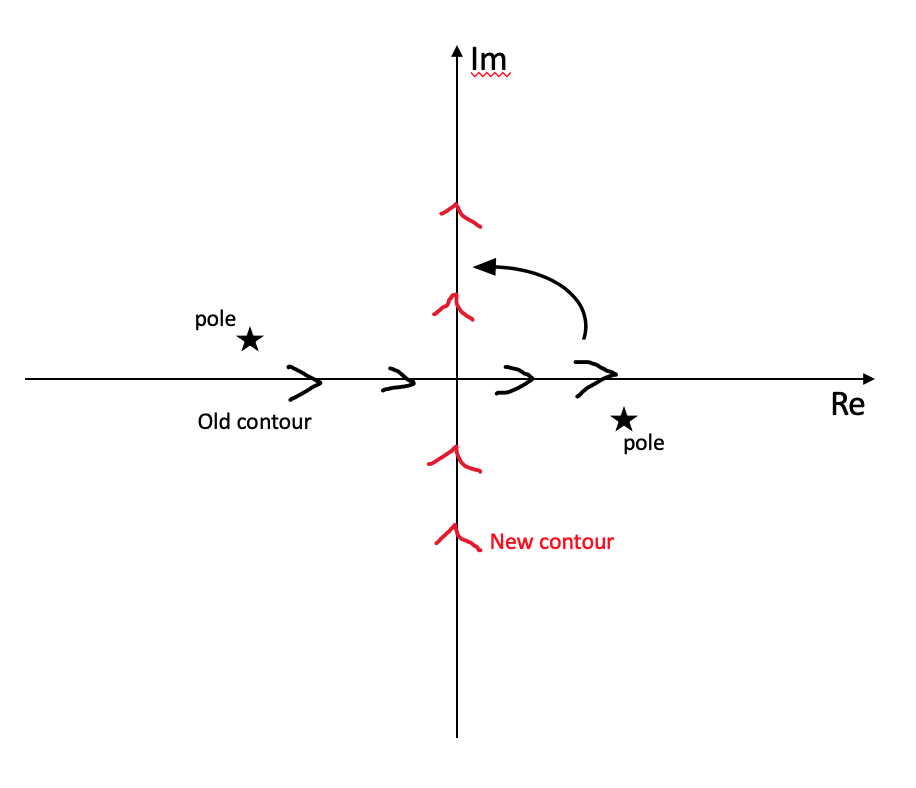
\includegraphics[width=3in]{images/contour.png}
	\caption*{Contour rotation from real-axis of $k_0$ to the imaginary axis of $k_0$.}
\end{figure}

\noindent Our integral is now

\begin{equation}
I_n(m) = -i \int \frac{d^{d-1} k}{(2 \pi)^d} \int^\infty_{-\infty} dk_0 \, \frac{1}{(k_0^2  + \omega^2)^n}.
\end{equation}

\noindent Where $\omega^2 = k^2 + m^2$. Reabsorb the time-component integral into the rest of the integrals, which we can interpret as $d$ Euclidean integrals, with the Euclidean metric, that will now exhibit spherical symmetry. Enter spherical polar coordinates

\begin{align}
I_n(m) &= -i \int_{\text{Euclidean}} \frac{d^d k}{(2 \pi)^d} \, \frac{1}{(k^2 + m^2)^n} \\
&= -\frac{i}{(2\pi)^d} \int d\Omega_d \int^\infty_0 dr \, \frac{r^{d-1}}{(r^2 + m^2)^n} \\
I_n(m) &= -\frac{i}{(2\pi)^d} \frac{(2\pi)^{\frac{d}{2}}}{\Gamma(\frac{d}{2})} \int^\infty_0 dr \, \frac{r^{d-1}}{(r^2 + m^2)^n} .
\end{align}

\noindent Make the change of variables $x = \frac{m^2}{r^2 + m^2}$

\begin{equation}
I_n(m) = \frac{m^{d-2n}}{(2\pi)^{\frac{d}{2}} \Gamma(\frac{d}{2})} \int_0^1 dx \, x^{n-\frac{d}{2}-1} (1-x)^{\frac{d}{2}-1}.
\end{equation}

\noindent This integral is a \textit{Beta function}!

\begin{equation}
I_n(m) = \frac{m^{d-2n}}{(2\pi)^{\frac{d}{2}} \Gamma(\frac{d}{2})}  \frac{\Gamma(n-\frac{d}{2}) \Gamma(\frac{d}{2})}{\Gamma(n)} = \frac{m^{d-2n}}{(2\pi)^{\frac{d}{2}}}  \frac{\Gamma(n-\frac{d}{2})}{\Gamma(n)}
\end{equation}

\noindent The gamma function has poles at negative integers, and this has divergences at $n=0,-1,-2,\dots$. The Feynman diagram expansion gives us $n$, and we are stuck with it. \\

\noindent What if $d$ is not a integer? This is the trick of dimensional regularization, as this renders the divergences finite. \\

\noindent Let $d = 4-\epsilon$, $\epsilon >0$, and study the behavior of the integral solutions as $\epsilon \rightarrow 0$.

\noindent As an example, consider the $n-2$ case (\textbf{Exercise})

\begin{align}
I_2 (m) &= \frac{m^{-\epsilon}}{(2\pi)^{2-\frac{\epsilon}{2}}} \Gamma \left(\frac{\epsilon}{2} \right) \\
&= \frac{1-\epsilon \text{log}(m)}{4\pi^2(1-\frac{\epsilon}{2} \text{log}(2\pi))} \left(\frac{2}{\epsilon} - \gamma \right) + \mathcal{O} (\epsilon^2)
\end{align}

\noindent Where $\gamma$ is the Euler-Mascheroni constant. This diverges as $\epsilon \rightarrow 0$, as expected, with the ``bad bit'' of $\frac{2}{\epsilon}$. \\

\noindent If we compare this with an integral that we've seen before, we can seee what kind of cutoff the free parameter $\epsilon$ is. Recall the diagram where we applied the momentum cutoff $|k| < \Lambda$. So, $\frac{1}{\epsilon} \sim \Lambda$.

\begin{figure}[H]
	\centering
	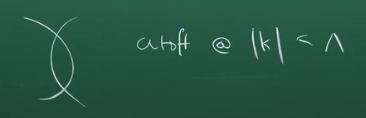
\includegraphics[width=2in]{images/firstcutoff.png}
\end{figure}


\clearpage

\section{Lecture 14: Quantization of Nonabelian Gauge Theory, Cont.}
\label{sec: lec14}


\noindent Working with nonabelian gauge theories, we've written down a Lagrangian density for Yang-mills theory, and after the gauge-fixing procedure of the Lagrangian density via path integrals and the tricks of Faddeev and Popov, we are ready to do some calculations. \\

\noindent The first topic to discuss is the \textit{beta function} or \textit{renormalization group equation}, which tells us how theories behave at low and high energies. The second topic to discuss is the departure from path integrals and gauge fixing to methods of lattice regulators, or cutoffs, for doing calculations in nonabelian gauge theory. \\

\subsection*{Renormalization of Nonabelian Gauge Theories}

\noindent We begin by reviewing renormalizability of quantum theories and the renormalization group equation, which tells us how coupling constants depend on the cutoff and how to adjust the coupling constants to match low and high energy predictions.  \\

\noindent Recall that a quantum theory $\hat{H}(z_1, \dots, z_n; \Lambda)$, where $\Lambda$ is the cutoff, data defined in a list of all the degrees of freedom of the theory, is renormalizable is it leads to finite predictions for all operationally well-defined observables. The expectation values of these observables must produce the same predictions for different choices of the chosen cutoff

\begin{equation}
\langle \hat{A}_j \rangle (z_1, \dots, z_n; K_c) \equiv f_j (z_1, \dots , z_n; K_c) = \alpha_j^{\text{obs.}}
\end{equation}

\noindent Where $K_c$ is a particular choice of cutoff: the length of list $\Lambda$, for example. This relationship of expectation values with different cutoffs yielding the same observed quantities is achieved in a renormalizable theory by allowing the coupling constants to depend on the cutoff $z_i  =z_i (K_c)$. \\

\noindent Apply the above equation to the Green's function, $n$-point correlation functions, where the dependency of the coupling constants and cutoff are implicit to the vacuum state $\ket{\Omega}$ and the dynamics of the field operators

\begin{align}
G^{(n)}(x_1, \dots, x_m; K_c) &\equiv \bra{\Omega} \mathcal{T} [\hat{\phi}(x_1) \dots \hat{\phi} (x_m) ] \ket{\Omega} \\
&\text{, where } \ket{\Omega} = \ket{\Omega(z_1, \dots , z_n; K_c)} \\
&\text{, and } \hat{\phi}(x) \equiv e^{-i \hat{H}(z_1, \dots, z_n; K_c)t} \hat{\phi}(0,\underline{x}) e^{i \hat{H}(z_1, \dots , z_n; K_c)t}.
\end{align}

\noindent So, we can equivalently say that a quantum theory $\hat{H}(z_1, \dots, z_n; \Lambda)$ is renormalizable if the correlation functions produce finite predictions for time-ordered quantities. \\

\noindent Now, to compute the relationship of $G^{(n)}$ to the coupling constants and the cutoff, consider changing the (usually) continuous parameter $K_c$ by an infinitesimal amount. Note that a common choice of cutoff could be $K_c = | p_{\text{max}} |$.

\begin{equation}
dG^{(n)} = \frac{\partial G^{(n)}}{\partial K_c} \delta K_c + \frac{\partial G^{(n)}}{\partial z_j} \delta z_j .
\end{equation}

\noindent So, the coupling constants $z_j (K_c)$ are chosen to fix $G^{(n)}$ with respect to transformations of the cutoff of the form $K_c \rightarrow K_c + \delta K_c$, but $G^{(n)}$ should not depend on $K_c$, and the above expression is equal to zero \\

\noindent To derive the \textit{renormalization group equation} or the \textit{beta function}, set the differential $dG^{(n)}$ to zero, divide by $\delta K_c$, and multiply by $K_c$

\begin{align}
\left[ K_c \frac{\partial}{\partial K_c} + K_c \frac{d z_j}{d K_c} \frac{\partial}{\partial z_j} \right] G^{(n)}&= 0 \\
\left[ K_c \frac{\partial}{\partial K_c} + \beta(z_j) \frac{\partial}{\partial z_j} \right] G^{(n)} &= 0 .
\end{align}

\noindent This is the infinitesimal form of the statement for a renormalizable theory that the Green's function shouldn't depend on the cutoff as it is changed, where 

\begin{equation}
\beta(z_j) = K_c \frac{d z_j}{d K_c} = \frac{d z_j}{d \, \text{ln} K_c}
\end{equation} 

\noindent Is the renormalization group or beta function, which allows us to compute the coupling constants in terms of the cutoff $z_j = z_j(K_c)$. The behavior of $\beta (z_j(K_c))$ is often used to describe the dependence of $z_j$ on $K_c$. \\

\subsection*{Aside: Massless Theories}

\noindent When we fix the Green's function to be equal to observable quantities, for any choice of cutoff, in a massive theory, we usually demand that the 2-point correlation function $\bra{\Omega} \hat{\phi} (p) \hat{\phi} (-p) \ket{\Omega}$ has a pole at the physical mass of the particle $m_{\text{phys}}$. \\

\noindent Complications arise in massless theories, as this leads to divergences, in the sense that we will end up with expressions like $\infty = \infty$. For massless theories, we instead insist that the 2-point correlation function has a pole at a negative, spacelike momenta $p^2 = -K_c^2 \equiv M^2$ with residue equal to one. This leads to finite predictions when we let $K_c \rightarrow \infty$.

\subsection*{Examples of Beta Functions}

\noindent (1) In $\phi^4$ theory, there is one coupling constant $\lambda$, the interaction strength, and the beta function is 

\begin{equation}
\beta(\lambda) = \frac{3 \lambda^2}{16 \pi^2} + \mathcal{O}(\lambda^3).
\end{equation}

\noindent (2) In quantum electrodynamics (QED), which is an abelian gauge theory, to first loop order, the beta function is 

\begin{equation}
\beta(e) = \frac{e^3}{12 \pi^2} + \mathcal{O}(e^4).
\end{equation}

\noindent Where $e$ is the electric charge of the particle. \\

\noindent (3) In Yang-Mills theory, a nonabelian gauge theory, there is more work to do in analyzing the divergences in the propagation of gauge bosons, as well as the propagation of fermions (quarks). The path integrals derived from applying the Yang-Mills theory Feynman rules produce divergences from the following terms in the Feynman expansion. See \textit{Peskin and Schroeder}, section 16.5 \textit{One-Loop Divergences of Non-Abelian Gauge Theory}, pages 521-544, for reference.

\begin{figure}[H]
	\centering
	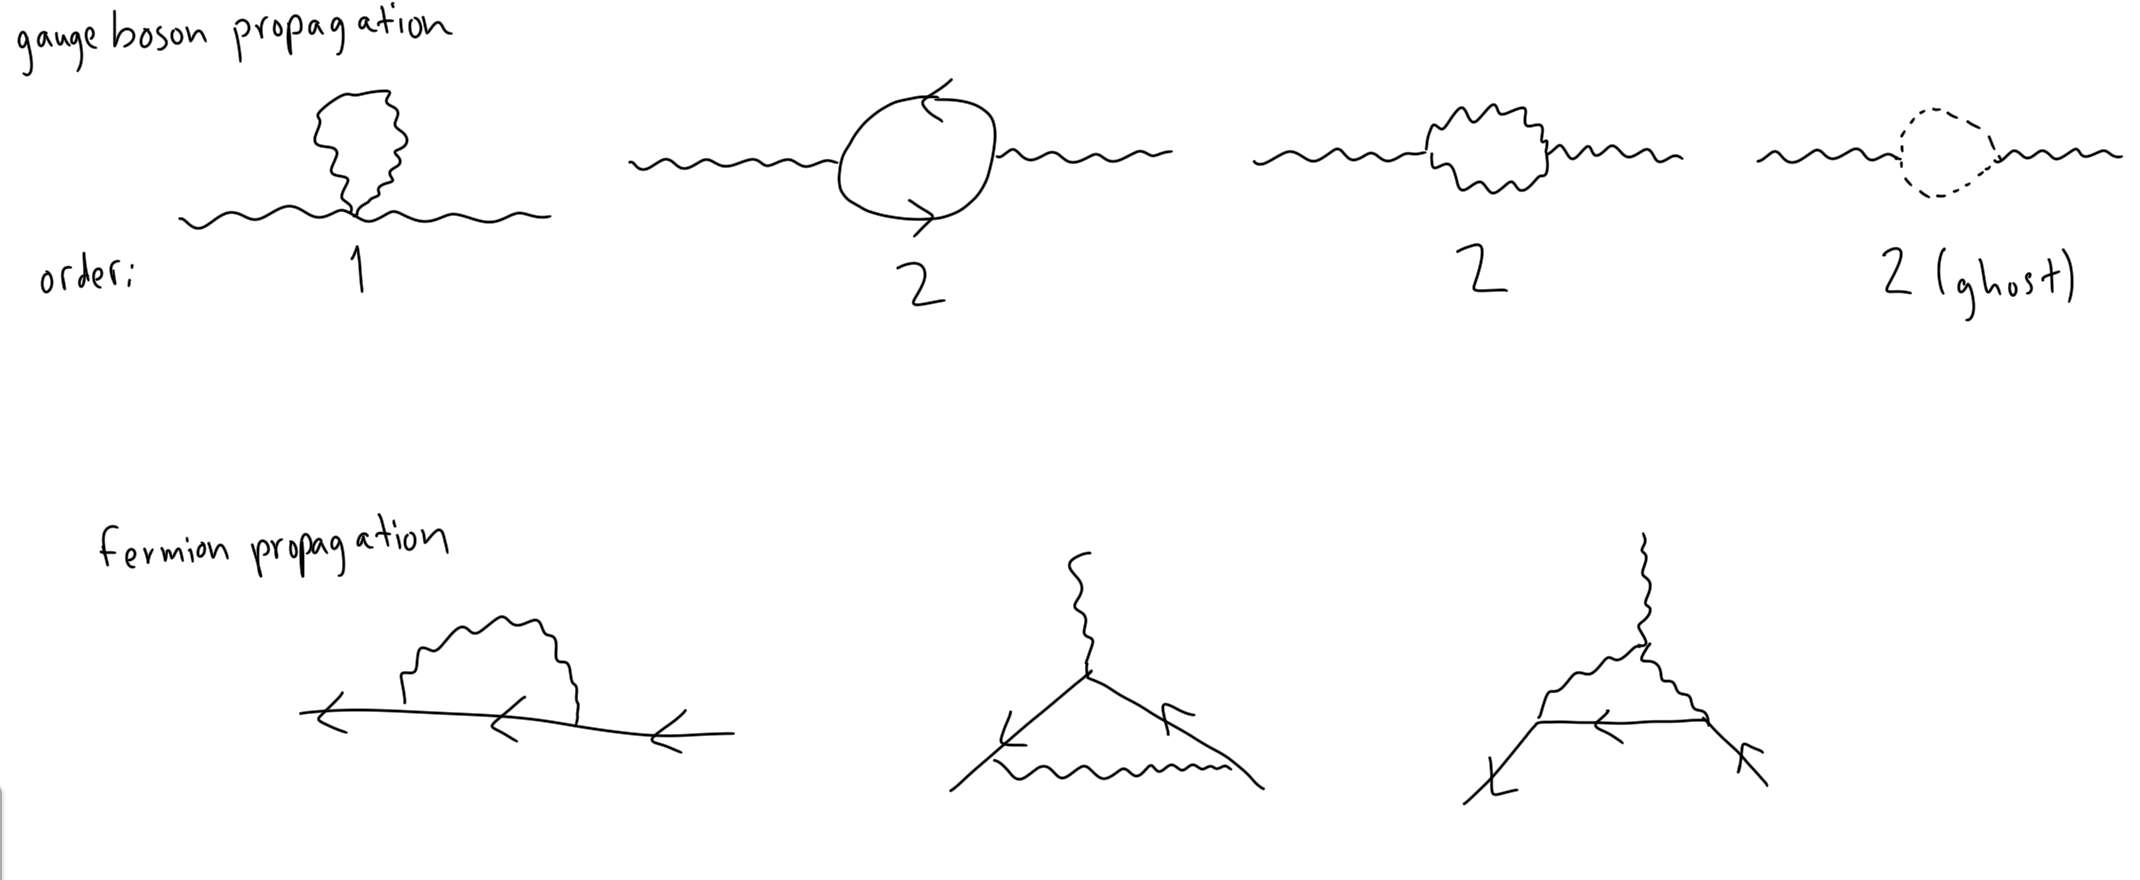
\includegraphics[width=5in]{images/beta_nagauge_div.png}
	\caption*{}
\end{figure}

\noindent To tame the infinities that arise from these diagrams, apply dimensional regularization to maintain Lorentz invariance and insist that each diagram leads to finite quantities. This then tells us what kinds of counter terms we need to add to the Lagrangian density for our theory, and, in turn, how the coupling constants change with respect to the cutoff. \\

\noindent This leads to the beta function for the $SU(N)$ local gauge group 

\begin{equation}
\beta(g) = - \frac{g^3}{16 \pi^2} \left( \frac{11 N}{3} - \frac{2 n_f}{3} \right)
\end{equation}

\noindent Where $n_f$ is the number of fermion families. Note that if $n_f$ is small, $\beta(g)$ becomes negative, and that $K_c \rightarrow \infty$ as $g$ gets smaller, meaning that our theory approaches being a free theory as $g \rightarrow 0$, and we can use perturbation theory for high-energy processes. This is called \textit{asymptotic freedom} of nonabelian gauge theories. \\

\subsection*{Low-Energy Physics of Nonabelian Gauge Theories}

\noindent Results here are thanks to Wilson's \textit{Confinement of Quarks} (1974). \\

\noindent To quantize an abelian or nonabelian gauge theory onto a discrete lattice, Wilson proposed the use of a lattice regulator. This is very challenging, since the gauge group acts on gauge fields like

\begin{equation}
A_\mu^j \frac{\sigma^j}{2} \rightarrow A_\mu^j \frac{\sigma^j}{2} + \frac{1}{g} (\partial_\mu \alpha^j) \frac{\sigma^j}{2} + i \left[\alpha^k \frac{\sigma^k}{2}, \alpha^l \frac{\sigma^l}{2}\right]
\end{equation}

\noindent And there any many complications in discretizing the derivative $\partial_\mu \alpha^j$ to the lattice. \\

\noindent Wilson recognized that the parallel transporter is the object that allowed us to do derivatives in the first place, and treated the parallel transporter 

\begin{equation}
U(j, j+\hat{e}^\mu) \in SU(2)
\end{equation}

as the fundamental degrees of freedom of the nonabelian gauge theory discretized to the lattice $\epsilon \mathbb{Z}^4$, instead of the gauge field.

\begin{figure}[H]
	\centering
	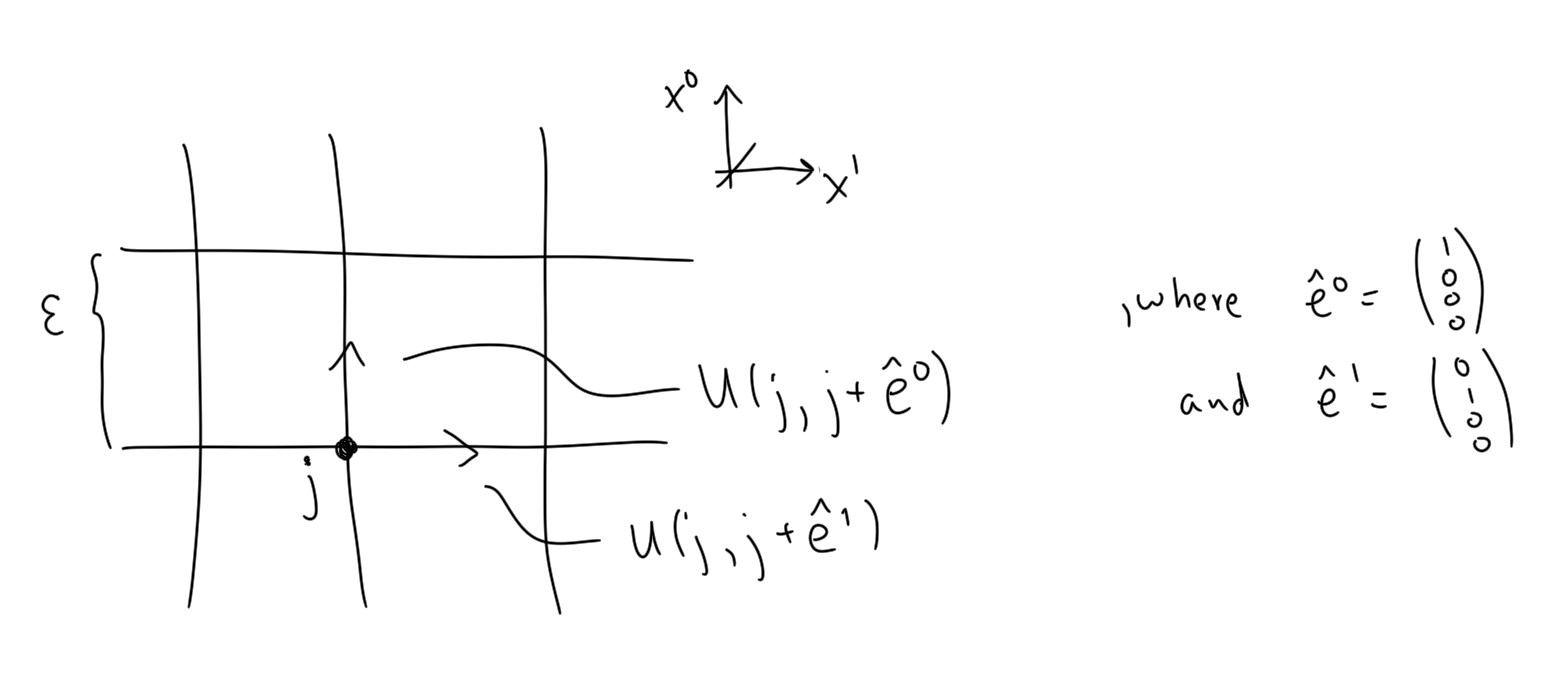
\includegraphics[width=4in]{images/wilson_parallel1.png}
	\caption*{}
\end{figure}

\noindent Bigger parallel transporters are built via multiplication. For example,

\begin{equation}
U(j, j+2\hat{e}^\mu) = U(j + \hat{e}^\mu, j+2\hat{e}^\mu)U(j, j+\hat{e}^\mu)
\end{equation}

\noindent These parallel transporters are $2 \times 2$ unitary matrices which populate the list of degrees of freedom, one for each link, or edge, in the classical lattice.\\

\noindent Side: Wilson ran calculations for the dynamics of a gauge field on a $4 \times 4 \times 4 \times 4$ lattice, which requires $4^4 \text{ lattice sites } \times 3 \text{ spatial coordinates per lattice site} = 768$ single-precision floating point numbers per unit time, requiring just 4 kilobytes of RAM. Note that a gigabyte ($\simeq 2^{30}$ bytes) of RAM is capable of storing $\sim 250,000,000$ single-precision floating point numbers, corresponding to almost $100 \times 100 \times 100 \times 100$ lattice. \\

\noindent To quantize the nonabelian gauge theory, Wilson proposed a way to build an action that summed over the plaquettes of the lattice, called \textit{Wilson loops}. In terms of the parallel transporters, the action has the form

\begin{equation}
S[U] = \sum_\Box \text{Wilson loops} = \sum_\Box \text{tr}(U_1 \cdot U_2 \cdot U_3 \cdot U_4)
\end{equation}

\noindent Where travelling around a plaquette may look like

\begin{figure}[H]
	\centering
	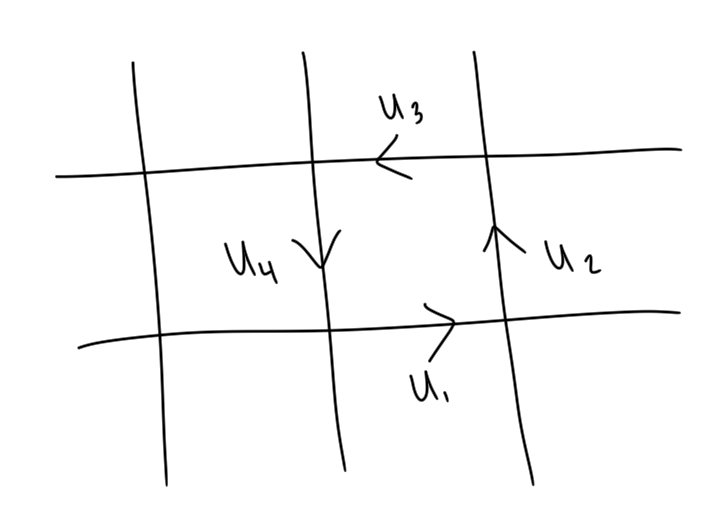
\includegraphics[width=2in]{images/wilson_parallel2.png}
	\caption*{}
\end{figure}

\noindent With this action, build the path integral $\int \mathcal{D}U \, e^{-iS[U]}$, and Wick rotate into the path integral $\int \mathcal{D}U \, e^{-S[U]}$ to work in imaginary time. Lastly, Monte Carlo sample the path integral. \\

\noindent This approach is actually the best way to get nonperturbative results in quantum field theory, but has its downsides: \\

\noindent Downside (1) is calculating processes in imaginary time is just like doing statistical mechanics with gauge theories at some defined temperature, and this is not good for time-ordered processes (e.g., scattering). Downside (2) is that this is not a quantum theory, as the Wilson loop is a classical configuration.

\subsection*{Hamiltonian Lattice Gauge Theory}

\noindent An alternative approach to quantization was introduced by Kogut and Susskind in 1975. They proposed a lattice quantum gauge theory, a quantum theory with a Hamiltonian and Hilbert space in which the degrees of freedom live on a lattice, which they argued yields Yang-Mills theory as the lattice spacing goes to zero. This is not proven, but if you can prove it, as well as that the low-energy limit has a mass cap, you can get a cool \$1M! \\

\noindent Recall that classically, each link, or edge, of the lattice is associated to a $2 \times2$ unitary matrix $U \in SU(2)$. In this lattice quantum gauge theory, each link or edge $e$ is associated to a wavefunction $\psi: \, SU(2) \rightarrow \mathbb{C}$, such that the wavefunction $\psi$ belongs the two-dimensional square-integrable functions on $SU(2)$ which is itself a Hilbert space per link $h_e$

\begin{equation}
\psi \in L^2 (SU(2)) \simeq h_e.
\end{equation}

\noindent Recall that $SU(2)$ is diffeomorphic to $S^3$, which conjures memories and solutions of wavefunctions on a sphere: spherical harmonics. \\

\noindent The total Hilbert space of this quantum theory is a tensor product over all the edges $e$ in the lattice $E$ of individual Hilbert spaces $h_e$

\begin{equation}
\mathcal{H} = \otimes_{e \in E} = \otimes_{e \in E} L^2 (SU(2)).
\end{equation}

\noindent To build the Hamiltonian, introduce some oeprations on the Hilbert space. First, write the states as kets in the position basis

\begin{equation}
\ket{\psi} = \int_{SU(2)} dU \, \psi (U) \ket{U}
\end{equation}

\noindent Where $\ket{U}$ is the position eigenvector defined by the three spatial coordinates. These states obey the inner product $\braket{U|V} = \delta(U-V)$. \\

\noindent Introduce the operators

\begin{equation}
L_U \ket{\psi} \equiv \int dV \, \psi (V) \ket{UV} \,\, \text{and} \,\, R_U \ket{\psi} \equiv \int dV \, \psi(V) \ket{VU^\dagger}.
\end{equation}

\noindent These operators are an analog of the shift operator $e^{ix \hat{p}}$. Note that $\ket{UV}$ is still a member of $SU(2)$. Differentiating these operators with respect to $U$ will yield momentum operators: dynamics.


\clearpage

\section{Lecture 15: Hamiltonian Lattice Gauge Theory}
\label{sec: lec15}


\noindent Continuing on the introduction to Hamiltonian lattice gauge theory as a means of quantization of gauge fields, we will build a microscopic formulation of gauge theory based on the real-space lattice. In contrast to the usual way of working on the Euclidean, Wick-rotated lattices, we will begin our theory with a Hamiltonian of classical degrees of freedom: namely, the parallel transporter $U$, a $2 \times 2$ matrix with determinant one, such that $U \in SU(2)$. Since we are working in 4D spacetime, we will have a 4D discretized lattice with lattice spacing $a \propto \frac{1}{K_c}$. In other words, 4D spacetime is discretized up to the cutoff $K_c$. \\ 

\noindent Like introduced before, each link, or edge, of the lattice $e \in E$, where $E$ is the set of all links of the lattice, has an associated parallel transporter, corresponding to the shortest, rectilinear path in between each vertex, $U_e \in SU(2) \simeq S^3$. Note that the parallel transporter is not a local object, as it is path dependent, implicitly depending on more than one coordinate. \\

\noindent The classical configuration space for this lattice gauge theory is a Cartesian product of $SU(2)$ per link in the lattice

\begin{equation}
\mathcal{C} = SU(2) \times SU(2) \times \dots \times SU(2).
\end{equation}

\noindent To quantize this classical lattice gauge theory, we'll begin by taking the simplest guess possible and introduce a wavefunction $\psi: \,\, \mathcal{C} \rightarrow \mathcal{C}$, where the Hilbert space has a ket basis $\ket{\psi} \in \mathcal{H} \simeq \otimes_{e \in E} h_e$, where $h_e$ is the space over each link. \\

\noindent Since $SU(2)$ is diffeomorphic to $S^3$, we are hinted towards defining wavefunctions as square-integrable functions on a sphere, and each point on the sphere will be associated to a complex number. Therefore, we define $h_e \equiv L^2(SU(2))$, where $L^2(SU(2))$ is an infinite-dimensional separable Hilbert space, since there are arbitrarily many orthogonal wavefunctions defined on the sphere. \\

\noindent Recall the two operators defined in $SU(2)$, for unitary matrix with unit determinant $U \in SU(2)$, that defined a right- and left-acting transformation

\begin{align}
&L_U : \,\, L^2 (SU(2)) \rightarrow L^2 (SU(2)) \\
&R_U : \,\, L^2 (SU(2)) \rightarrow L^2 (SU(2))
\end{align}

\noindent Where $L_U$ and $R_U$ commute, such that $[L_U, R_U]=0$, and form the representation defined by the relations 

\begin{equation}
L_U^\dagger L_U = R_U^\dagger R_U = \mathbb{I} \text{ and } L_{UV} = L_U L_V.
\end{equation}

\noindent To understand how the infinite-dimensional Hilbert space $L^2(SU(2))$ breaks up into a direct sum of irreducible representations of $SU(2)$, we invoke the third part of the \textit{Peter-Weyl therorem}, which states that the Hilbert space over $SU(2)$ consisting of square-integrable functions may be regarded as a representation of a direct product of left- and right-acting operators, and the Hilbert space decomposes into an orthogonal direct sum of all the irreducible unitary representations, with multiplicity of each irreducible representation equal to its degree, the dimension of the underlying space of that representation (See Wikipedia page on Peter-Weyl theorem for overview). We write this all as \\

\begin{equation}
h_e \equiv L^2(SU(2)) \simeq \bigoplus_{l \in \frac{1}{2}\mathbb{Z}^+} \,\, V_l \otimes V_l^* \simeq \bigoplus_{l \in \frac{1}{2}\mathbb{Z}^+} \,\, \mathbb{C}^{2l+1} \otimes \mathbb{C}^{2l+1}
\end{equation}

\noindent Where $V_l \simeq \mathbb{C}^{2l+1}$ is the $(2l+1)$-dimensional vector space furnishing the irreducible representation of $SU(2)$ of spin, or angular momentum $l$ and $\frac{1}{2}\mathbb{Z}^+ = \{0,\frac{1}{2},1,\frac{3}{2},2,\dots\}$. \\

\noindent Now to find a representation of $SU(2)$ on this vector space $V_l$, we'll use a piece of Lie group representation theory not found in any textbook. Note that the action of $SU(2)$ generates a representation

\begin{equation}
\Pi_l (SU(2)) : \,\, V_l \rightarrow V_l.
\end{equation}

\noindent In the procedure to calculate the matrix $\Pi_l (SU(2))$, we will use two pieces of machinery

\begin{itemize}
\item The spin-$\frac{1}{2}$ fundamental representation of $SU(2)$
	\subitem $\Pi_{\frac{1}{2}} (U) = \left(\begin{array}{cc} a & b \\ c & d \end{array}\right)$
\item Tensor products of the spin-$\frac{1}{2}$ 2D vector spaces furnishing the fundamental representation of $SU(2)$, $V_{\frac{1}{2}} \simeq \mathbb{C}^2 \equiv \{ \ket{0}, \ket{1} \}$.
\end{itemize}

\noindent Begin the procedure to get the matrix representation for any spin-$l$, take the tensor product of $n$ of the spin-${\frac{1}{2}}$ fundamental vector spaces 

\begin{equation}
V_{\frac{1}{2}} \otimes V_{\frac{1}{2}} \otimes \dots \otimes V_{\frac{1}{2}}.
\end{equation}

\noindent Note that for quantum computer fans, this is the vector space of $n$ qubits

\begin{equation}
V_{\frac{1}{2}} \otimes V_{\frac{1}{2}} \otimes \dots \otimes V_{\frac{1}{2}} \simeq \mathbb{C}^2 \otimes \dots \otimes \mathbb{C}^2 = \mathcal{C}^{2^n}.
\end{equation}

\noindent The spin-$l$ representation $\Pi_l(U)$, generated from $SU(2)$ action on $V_l$, lives in thsi tensor product space of $n$ copies of $V_{\frac{1}{2}}$, as long as $n=2l$ or $l=\frac{n}{2}$. Therefore, we will build $V_l$ as a subspace of this tensor product space, most fo which will be thrown away once we find our subspace of interest, by building a set a $n+1$ orthonormal vectors

\begin{align}
\ket{w_{\frac{n}{2}}} &= \ket{1 1 \dots 1} \\
\ket{w_{\frac{n}{2}-1}} &= \frac{1}{\sqrt{n}} \left( \ket{1 1 \dots 1 0} + \ket{1 1 \dots 1 0 1} + \dots + \ket{0 1 \dots 1} \right) \\
\dots& \\
\ket{w_{\frac{n}{2}-k}} &= \frac{1}{\sqrt{n \choose k}} \left( \ket{ 1 \dots 1 0 \dots 0} + \text{(all permutations of $k$ zeros and $n-k$ ones)} \right) \\
\dots& \\
\ket{w_{-\frac{n}{2}}} &= \ket{ 0 0 \dots 0}.
\end{align}

\noindent Then the matrix elements of the representation $\Pi_l (U)$ are simply given by the expectation value on $n$ copies of $U$ in this orthonormal basis

\begin{equation}
[\Pi_l (U) ]_{jk} = \bra{w_j} U \otimes \dots \otimes U \ket{w_k}
\end{equation}

\noindent Where $j, \, k \in \{ -\frac{n}{2}, \dots, \frac{n}{2} \}$. \\

\noindent Note that this method is good and fast for low spin representations, but clearly gets unwieldy for working with the Hilbert space of $n=1000$ qubits, and the efficiency and value of the methods of addition of angular momentum and Clebsch-Gordan coefficients, with the raising and lower operators, the highest-weight vectors, etc. \\

\noindent Sticking to low spin representations for our purposes, we can start to extract matrix representations for $l=0$, $l=\frac{1}{2}$, and $l=1$. \\

\noindent For $l=0$, the matrix representation is just the identity

\begin{equation}
\Pi_0 (U) = \mathbb{I}.
\end{equation}

\noindent For $l=\frac{1}{2}$, we have the fundamental matrix representation 

\begin{equation}
[\Pi_{\frac{1}{2}} (U) ]_{jk} = [U]_{jk}.
\end{equation}

\noindent In the $l=1$ subspace, there are three orthonormal basis vectors

\begin{equation}
\{ \ket{w_1} = \ket{1 1}, \,\, \ket{w_0} = \frac{1}{\sqrt{2}} (\ket{1 0} + \ket{0 1}), \,\, \ket{w_{-1}} = \ket{0 0} \}.
\end{equation}

\noindent The matrix elements are then gotten by the expectation value above, pulling values from the fundamental representation

\begin{align}
[\Pi_1 (U) ]_{11} &= \bra{1 1} U \otimes U \ket{1 1} = \bra{1} U \ket{1} \bra{1} U \ket{1} = a^2 \\
[\Pi_1 (U) ]_{00} &= \frac{1}{2} \left( \bra{1 0} U \otimes U \ket{1 0} + \bra{1 0} U \otimes U \ket{0 1} + \bra{0 1} U \otimes U \ket{1 0} + \bra{0 1} U \otimes U \ket{0 1} \right) \\
 &= ad + bc.
\end{align}

\noindent Recall that the Peter-Weyl theorem tells us that the Hilbert space of square-integrable functions on $SU(2)$ is isomorphic to the infinite-dimensional, until we truncate, direct sum space of $(2l+1)$-dimensional vector spaces furnishing the representation of $SU(2)$

\begin{equation}
L^2 (SU(2)) \simeq \bigoplus_{l \in \frac{1}{2}\mathbb{Z}^+} \,\, \mathbb{C}^{2l+1} \otimes \mathbb{C}^{2l+1}.
\end{equation}

\noindent And $SU(2)$ acts on $L^2 (SU(2))$ via the operator $L_U: \, L^2 (SU(2)) \rightarrow L^2 (SU(2))$ with action

\begin{equation}
L_U \simeq \bigoplus_{l \in \frac{1}{2}\mathbb{Z}^+} \,\, \Pi_l (U) \otimes \mathbb{I}.
\end{equation}

\noindent The elements of the matrix representation $[\Pi_l (U)]_{jk} \equiv t^l_{jk} (U)$ are square-integrable functions from $SU(2)$ to the complex numbers $\mathbb{C}$, since $SU(2)$ is compact, and form an orthogonal (not orthonormal) basis for $L^2 (SU(2))$, where $-l \le j,k \le l$. So, we can expand the wavefunction ket in the orthogonal basis of the matrix elements

\begin{equation}
\ket{\psi} = \sum_l \sum_{j,k} \psi^l_{jk} \ket{j}_l \ket{k}_l = \sum_l \sum_{j,k} \psi^l_{jk} \sqrt{2l+1} \ket{t^l_{jk}}.
\end{equation}

\noindent The inner product of the Hilbert space $L^2 (SU(2))$ is defined with the Haar measure $\int dU$ by

\begin{equation}
(\psi, \phi) \equiv \int dU \, \psi^* (U) \phi(U)
\end{equation}

\noindent Where we use the inner product of the orthogonal basis vectors, where integrals over $SU(2)$ with the Haar measure behave like $\int dU \, U \otimes U^\dagger \propto \mathbb{I} \otimes \mathbb{I} + (\text{swap operations})$, and (\textbf{Exercise})

\begin{equation}
(t^l_{jk}, t^{l'}_{j'k'}) = \delta^{ll'} \delta_{jj'} \delta_{kk'} \frac{1}{2l+1}.
\end{equation}

\noindent Therefore, the basis for the total Hilbert space consists of wavefunctions $\ket{\Psi} \in \mathcal{H}$ and

\begin{equation}
\ket{\Psi} = \sum_{l_1 l_2 \dots} \sum_{j_1 j_2 \dots} \sum_{k_1 k_2 \dots} \, \Psi^{l_1 l_2 \dots}_{j_1 j_2 \dots k_1 k_2 \dots} \ket{j_1}_{l_1} \ket{k_1}_{l_1} \ket{j_2}_{l_2} \ket{k_2}_{l_2} \dots .
\end{equation}

\noindent To give dynamics to the Hilbert space, we define some observables. Consider an element of $SU(2)$, $U=e^{c_j \tau^j}$, where $c_j \tau^j$ are elements of the Lie algebra of $SU(2)$, $c_j \in \mathbb{R}^3$, and $\tau^j$ are the Pauli spin matrices multiplied by i and divided by 2 for normalization conditions. The spin matrices obey the commuation relations $[\tau^j,  \tau^k] = -2 \epsilon^{jk}_{\,\,\,\,l} \tau^l$. We can recover the spin matrix from the group element via differentation

\begin{equation}
\frac{d U}{d c_j} \Big{|}_{c_j = 0} = \tau^j.
\end{equation}

\noindent The first observable we define is the anti-Hermitian \textit{left angular momentum operator}

\begin{equation}
\hat{l}_L^j \equiv \frac{d}{ds} L_{U=e^{s\tau^j}} \Big{|}_{s=0}.
\end{equation}

\noindent Note that this is a factor of $i$ away from being Hermitian, and is analogous to the Hermitian linear momentum operator $i\hat{p}$. Also, notice that we begin with a unitary operator $L_U$, apply an anti-Hermitian operator $\frac{d}{ds}$, and kill off the unitarity by setting $s=0$ after the derivative. \\

\noindent The second observable we define, similar to the first, is the \textit{right angular momentum operator}

\begin{equation}
\hat{l}_R^j \equiv \frac{d}{ds} R_{U=e^{s\tau^j}} \Big{|}_{s=0}.
\end{equation}

\noindent Next, define the position observable $\hat{U}_{jk}$, which is also a map $L^2 (SU(2)) rightarrow L^2 (SU(2))$ and yields the fundamental representation matrix elements when it acts on the position eigenkets $\ket{U}$ of $SU(2)$.

\begin{equation}
\hat{U}_{jk} \ket{U} = [\Pi_{\frac{1}{2}} (U) ]_{jk} \ket{U}.
\end{equation}

\noindent Acting the position operator on the Hilbert space wavefunctions $\ket{\psi} = \int dU \, \psi(U) \ket{U}$, we get the Haar integral over position eigenkets

\begin{equation}
\hat{U}_{jk} \ket{\psi} = \int dU \, \psi(U) [\Pi_{\frac{1}{2}} (U)]_{jk} \ket{U} = \int dU \, \psi(U) t^{l=\frac{1}{2}}_{jk} (U) \ket{U}.
\end{equation}

\noindent To build the Hamiltonian, kinetic energy plus potential energy, we use the plaquette operator to define parallel transport on the 4D lattice

\begin{align*}
\hat{U}_\Box : \,\, &L^2 (SU(2)) \otimes L^2 (SU(2)) \otimes L^2 (SU(2)) \otimes L^2 (SU(2)) \\
&\rightarrow L^2 (SU(2)) \otimes L^2 (SU(2)) \otimes L^2 (SU(2)) \otimes L^2 (SU(2))
\end{align*}

\noindent We choose the convention to set arrows on each link running ``left-to-right'' and ``down-to-up'' in the plane of the ``paper'', and then walk around the plaquette counterclockwise (CCW), taking the Hermitian conjugate of the parallel transporter if we are traveling against the arrow. The parallel transporter for each link is considered the observable for that link when traveling around the plaquette. Each link are labeled by $e_i$, $i=1,2,3,4$. \\

\begin{figure}[H]
	\centering
	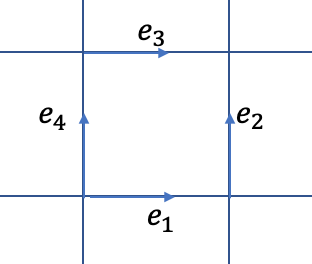
\includegraphics[width=1.5in]{images/ks_plaquette.png}
	\caption*{}
\end{figure}

\noindent Build an operator that acts on the 4D space of links, as a sum over the links of the direct products of parallel transporters

\begin{equation}
\hat{M}_{\Box; j_1, k_4} = \sum_{k_1, k_2, k_3} \hat{U}_{j_1 k_1} \otimes \hat{U}_{k_1 k_2} \otimes \hat{U}_{k_2 k_3}^\dagger \otimes \hat{U}_{k_3 k_4}^\dagger.
\end{equation}

\noindent This is then turned into an observable by summing over the last, initially-fixed index $k_4$

\begin{equation}
tr(\hat{U}_\Box) \equiv \sum_{k_4} \hat{M}_{\Box; k_4, k_4}.
\end{equation}

\noindent Note that $tr(\hat{U}_\Box)$ is a trace operator that acts on $L^2 (SU(2)) \otimes L^2 (SU(2)) \otimes L^2 (SU(2)) \otimes L^2 (SU(2))$, and \textbf{not} a number! \\

\noindent Put the defined observables together into the \textit{Kogut-Susskind Hamiltonian}

\begin{equation}
\hat{H}_{KS} = -\frac{g_H^2}{2a} \sum_{e \in E} \, \hat{l}_L^j (e) \hat{l}_L^j (e) + \frac{1}{2 g_H^2 a} \sum_{\text{plaquettes } \Box} \, \left(tr(\hat{U}_\Box) + \text{Hermitian conjugate} \right)
\end{equation}

\noindent Where $g_H$ is the coupling constant. \\

\noindent This model has a huge group of gauge symmetries. \\

\noindent Consider a vertex in the lattice and build the operator

\begin{figure}[H]
	\centering
	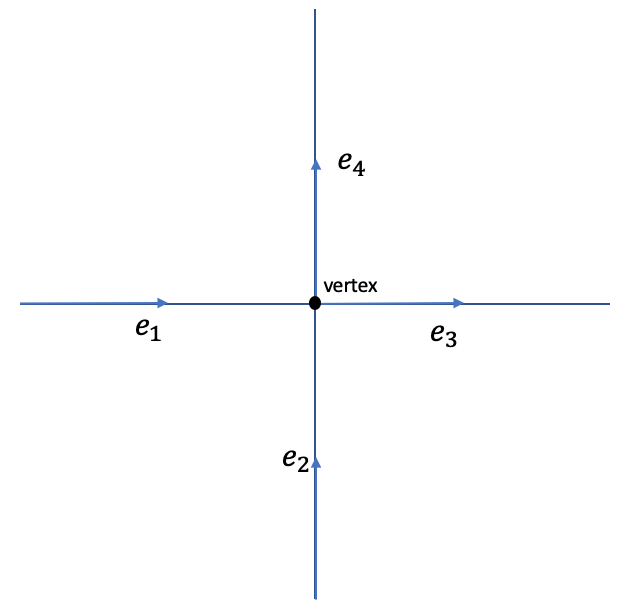
\includegraphics[width=3in]{images/ks_vertex.png}
	\caption*{}
\end{figure}

\begin{equation}
M_x \equiv R_x (e_1) \otimes R_x (e_2) \otimes L_x (e_3) \otimes L_x (e_4)
\end{equation}

\noindent Where $x \in SU(2)$. These operators obey the following commutation relations 

\begin{equation}
[M_x (v), M_y (w)] = 0 \text{ and } [M_x (v), \hat{H}_KS] = 0 \text{, for all } x, y, v, w.
\end{equation}

\noindent In summary, Wilson's formulation received much more attention at the time for its ease of discretizstion, translation to computer programs, and use of Monte Carlo sampling, which classical computers are good at. Kogut and Susskind argued that the plaquette operator becomes the curvature term, as expected, in the small lattice spacing $a$ limit in their theory, as well as that hte kinetic energy term becomes the kinetic energy in the timelike direction of the curvature term. The Kogut-Susskind formulation may be very promising for quantum simulations done by quantum computers, which are not very good at sampling techniques, but excel in simulating the dynamics of local lattice models.

\clearpage

\section{Lecture 16: Spontaneous Symmetry Breaking}
\label{sec: lec16}

\noindent This is the last topic that we need to complete our description of the standard model of elementary particle interactions. \textit{Spontaneous symmetry breaking} (SSB) is an observed behavior within field theories, and we will begin with some examples of classical SSB.

\subsubsection*{Particle in a double well example}

\noindent Consider a classical particle confined to a double-well potential with Hamiltonian

\begin{equation}
H = \frac{p^2}{2m} + V(x).
\end{equation}

\noindent This system posses $\mathbb{Z}_2$ symmetry in its solutions, since $x \rightarrow -x$ is a symmetry operation. Note that the particle in this potential at $x=0$ must choose a positive or negative local minimum, meaning that the ground state is degenerate and breaks the $\mathbb{Z}_2$ symmetry. \\

\begin{figure}[H]
	\centering
	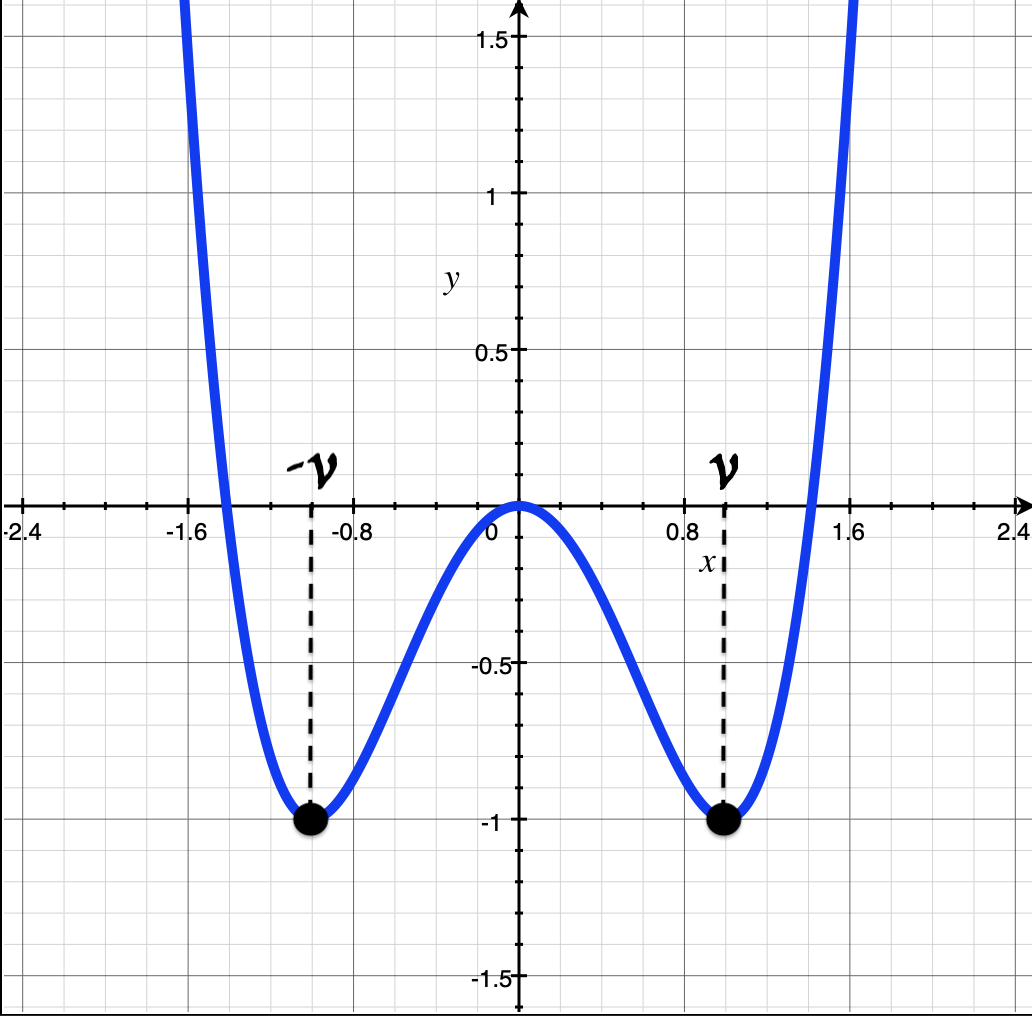
\includegraphics[width=3in]{images/mexhat2d.png}
	\caption*{Potential exhibiting $\mathbb{Z}_2$ symmetry.}
\end{figure}

\noindent The quantum analog of this classical theory does not exhibit SSB, since the ground state wavefunction is symmetric, but the first excited state is antisymmetric.

\begin{figure}[H]
	\centering
	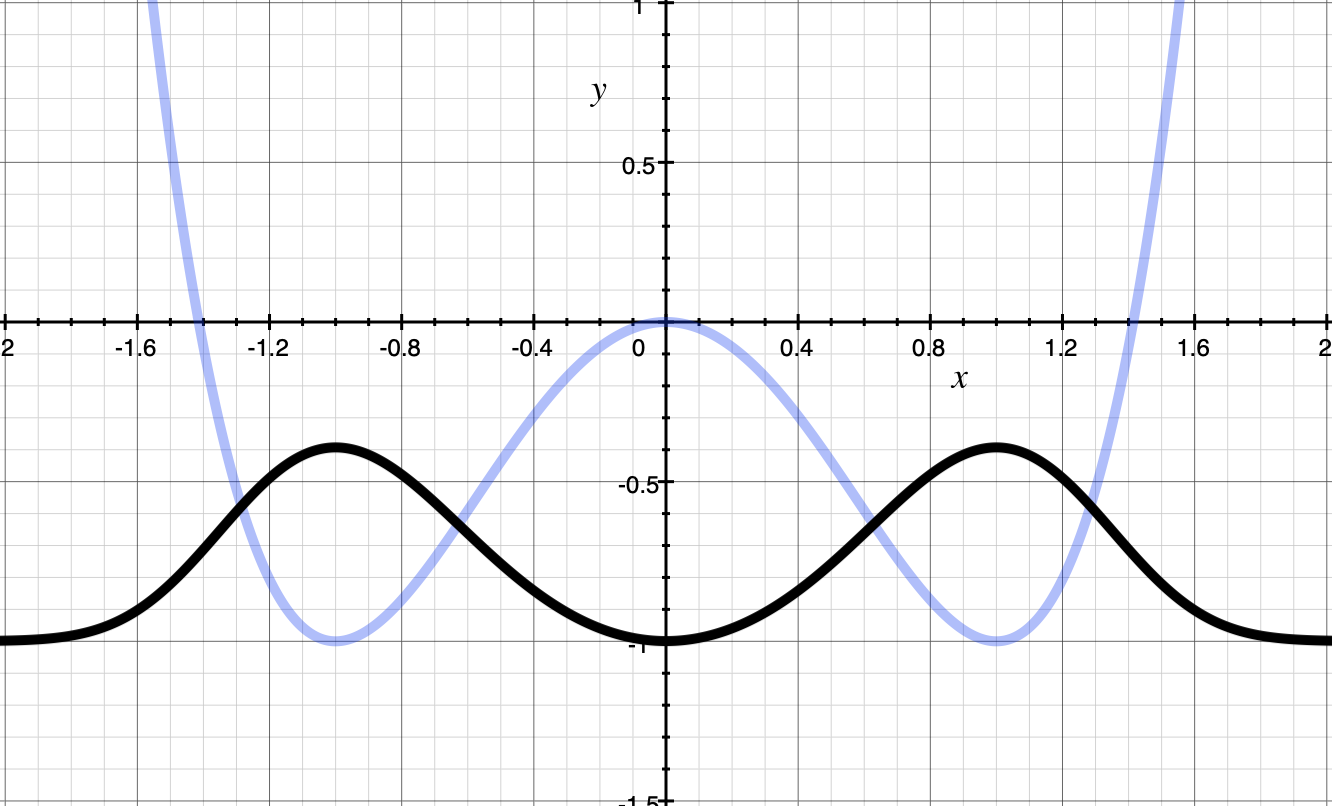
\includegraphics[width=2in]{images/mexhat2d_ground.png}
	\caption*{Symmetric ground state wavefunction.}
\end{figure}

\begin{figure}[H]
	\centering
	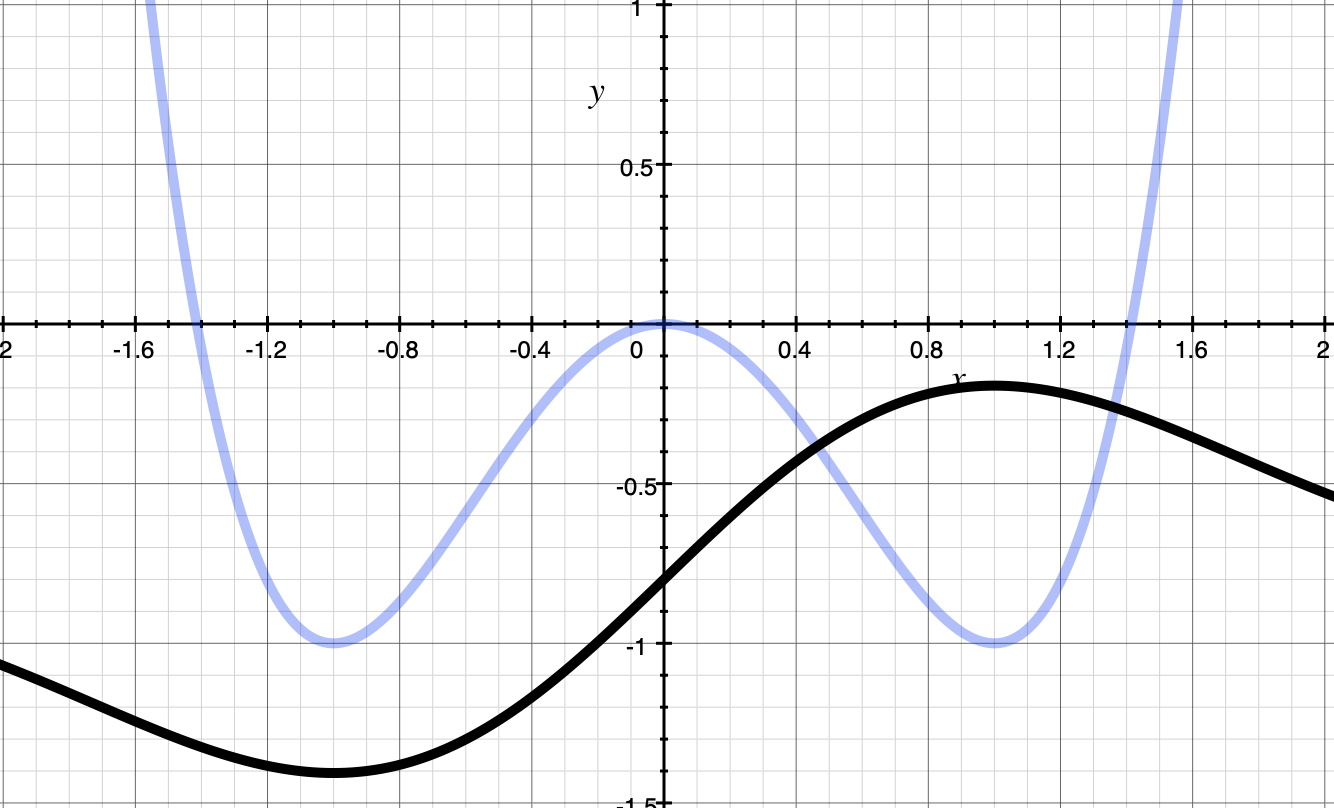
\includegraphics[width=2in]{images/mexhat2d_first.png}
	\caption*{Antisymmetric first excited state wavefunction.}
\end{figure}

\subsubsection*{Ising model (statistical physics) example}

\noindent The Ising model is a model of ferromagnetic materials, where spins can point up or down, corresponding to a spin value $s_j =  \pm 1$, with a Hamiltonian containing the pairwise summation

\begin{equation}
H = -\sum_{\langle jk \rangle} s_j s_k.
\end{equation}

\noindent This theory contains two ground states: all spins pointing up or all pointing down, and possesses $\mathbb{Z}_2$ symmetry by the operation $s_j \rightarrow -s_j$. \\

\noindent Depending on the temperature, the thermal state of this system can be in one of two regimes: critical or non-critical. Consider the Gibbs, or mixed, state density operator describing the system at any temperature

\begin{equation}
\rho = \frac{e^{-\beta H}}{Z}
\end{equation}

\noindent Where $Z$ is the partition function and $\beta = \frac{1}{k_B T}$ is the temperature factor. Note that the Gibbs state is all $\mathbb{Z}_2$ symmetric, meaning that it does break any symmetries. Now there exists a critical temperature $\beta_{c}$, below which the system becomes ordered due to small external magnetic fluctuations and symmetry is broken. Above the critical temperature, the system is disordered with random thermal fluctuations. As $\beta \rightarrow \infty$,

\begin{equation}
\rho = \left(\frac{1}{2} - \epsilon\right) (\text{all up states}) + \left(\frac{1}{2} - \epsilon \right)(\text{all down states}).
\end{equation}

\subsubsection*{Classical field theory example}

\noindent Consider the Lagrangian density, much like the $\phi^4$ interacting theory we've encountered, but the ``mass'' term is made negative and $m \rightarrow \mu$

\begin{equation}
\mathcal{L} = \frac{1}{2} (\partial_\mu \phi)(\partial^\mu \phi) + \frac{1}{2} \mu^2 \phi^2 - \frac{\lambda}{4!} \phi^4.
\end{equation}

\noindent Note that measurable quantities are usually functions of the parameters, making this a perfectly fine theory. We then have the Hamiltonian

\begin{equation}
H = \int d^3 x \, \left( \frac{1}{2} \pi^2 + \frac{1}{2} (\nabla \phi)^2 - \frac{1}{2} \mu^2 \phi^2 + \frac{\lambda}{4!} \phi^4 \right).
\end{equation}

\noindent To uncover the $\mathbb{Z}_2$ symmetry of this theory, minimize the Hamiltonian with respect to the field $\phi$, making all derivatives of $\phi$ equal to zero, and calculate the configuration with the smallest energy. The extremum condition for the remaining potential energy terms

\begin{equation}
\frac{\partial V(\phi)}{\partial \phi} = -\mu^2 \phi + \frac{\lambda}{6} \phi^3 = 0
\end{equation}

\noindent Yields three configurations that extremize the energy of the system. Namely, for $\phi = 0$ and $\phi = \pm \sqrt{\frac{6 \mu^2}{\lambda}}$. The quantum analog of this theory also exhibits SSB.

\subsubsection*{Quantum field theory example: transverse Ising model}

\noindent Consider the quantum theory of a 1D lattice of spins, which also exhibits $\mathbb{Z}_2$ symmetry, with the Hamiltonian

\begin{equation}
\hat{H} = - \sum_{j} \sigma_j^x \sigma_{j+1}^x + h \sum_j \sigma_j^z
\end{equation}

\noindent Where the first term is the neighboring interaction and the second term is the magnetic interaction with $h$ as the magnetic field strength, and the Pauli spin matrices

\begin{equation}
\sigma^x = \left( \begin{array}{cc} 0 & 1 \\ 1 & 0 \end{array} \right) \text{ and } \sigma^z = \left( \begin{array}{cc} 1 & 0 \\ 0 & -1 \end{array} \right).
\end{equation}

\noindent The Hamiltonian exhibits $\mathbb{Z}_2$ symmetry, since 

\begin{equation}
[\Phi,\hat{H}] = 0 \text{ for } \Phi = \dots \sigma_j^z \sigma_{j+1}^z \dots.
\end{equation}

\noindent The basis for the $h=0$ ground state can be written as

\begin{align}
\ket{\Omega_+} &\equiv \ket{+} \otimes \ket{+} \otimes \dots \otimes \ket{+} \\
\ket{\Omega_-} &\equiv \ket{-} \otimes \ket{-} \otimes \dots \ket{-}
\end{align}

\noindent Where the individual spin states are

\begin{equation}
\ket{+} = \frac{1}{\sqrt{2}} \left( \ket{0} + \ket{1} \right) \text{ and } \ket{-} = \frac{1}{\sqrt{2}} \left( \ket{0} - \ket{1} \right).
\end{equation}

\noindent The $h=0$ ground state eigenspace is twofold degenerate with the above basis. A good, non-degenerate ground state, for example, could be $\frac{1}{\sqrt{2}} ( \ket{\Omega_+} \pm \ket{\Omega_-} )$, but these states are never seen in experiment, since decoherence destroys any superpositions of states. Neither state by itself exhibits the symmetry, but one state must be chosen by measurement. The only information we have about the two states' relationship is $\Phi \ket{\Omega_+} = \ket{\Omega_-}$.

\subsubsection*{Continuous SSB Example: Linear $\sigma$-model}

\noindent Consider the Lagrangian density for an effective model of pions that exhibits SSB of a continuous symmetry

\begin{equation}
\mathcal{L} = \frac{1}{2}(\partial_\mu \phi^j )^2 + \frac{1}{2} \mu^2 (\phi^j)^2 - \frac{\lambda}{4!} (\phi^j)^4
\end{equation}

\noindent Where $(\phi^j)^2 = \sum_{j=1}^N \phi^j \phi^j$. The dynamics of the $N$ independent (Klein-Gordon) scalar field are invariant under orthogonal rotations $O \in O(N)$, a continuous group of symmetries, such that

\begin{equation}
O: \,\, \phi^j \rightarrow [O]^j_k \phi^k.
\end{equation}

\noindent What is the lowest energy configuration? Minimize the potential energy $V(\phi^j) = -\frac{1}{2} \mu^2 (\phi^j)^2 + \frac{\lambda}{4!} (\phi^j)^4$ with respect to $\phi^j$, showing that the minimum occurs for any constant configuration of the fields that satisfies the equation (\textbf{Exercise})

\begin{equation}
(\phi_0^j)^2 = \frac{\mu^2}{\lambda}. 
\end{equation}

\noindent There is more than one energy configuration that leads to this solution, including superpositions of the following vectors

\begin{equation}
\begin{pmatrix} \frac{\mu}{\sqrt{\lambda}} \\ 0 \\ 0 \\ \dots \\ 0 \end{pmatrix}, \begin{pmatrix} 0 \\\frac{\mu}{\sqrt{\lambda}} \\ 0 \\ \dots \\ 0 \end{pmatrix}, \dots .
\end{equation}

\noindent In the case of $N=2$, the potential energy minima form the ``wine bottle'' or ``mexican hat'' potential. The minimum energy configurations are points on this potential and form circles around the indent of the ``bottom of the bottle''. In other words, any configuration that lands on the circle is a minimum energy configuration.

\begin{figure}[H]
	\centering
	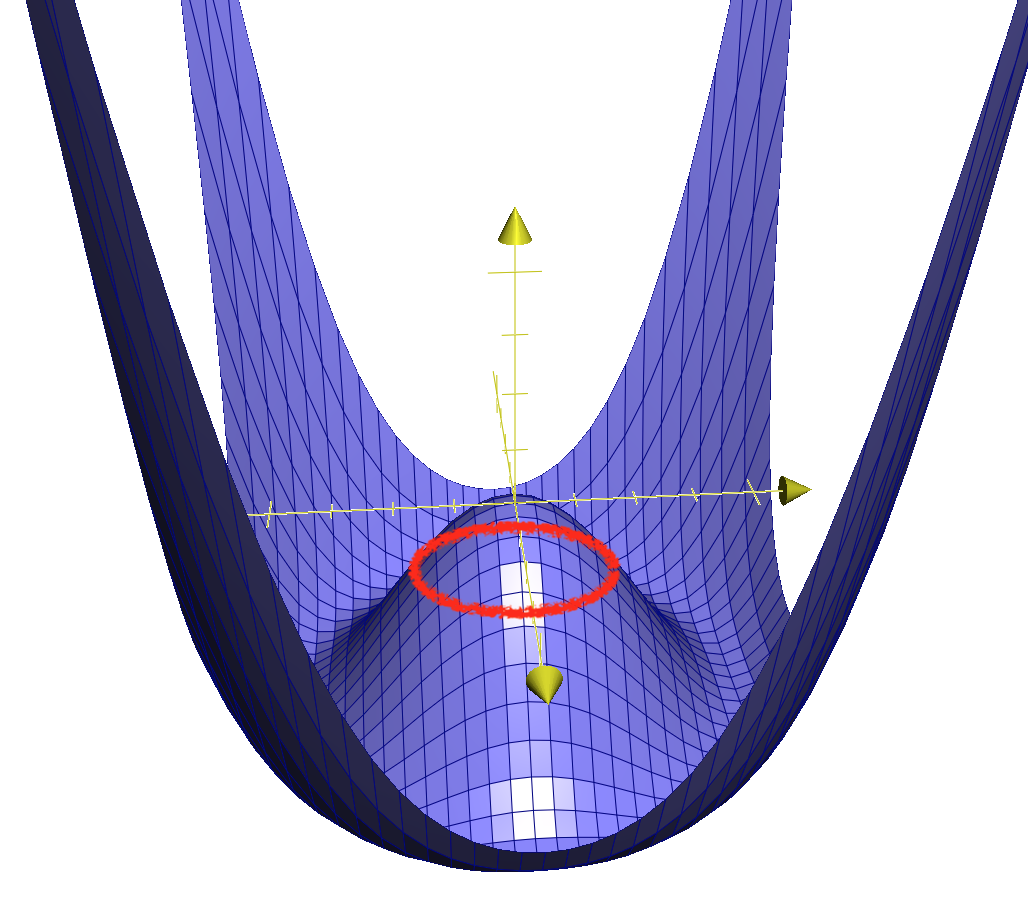
\includegraphics[width=3in]{images/mexhat3d.png}
	\caption*{Mexican hat potential of the linear sigma model.}
\end{figure}

\subsubsection*{Low Energy Dynamics for SSB}

\noindent To study the dynamics as we start to depart from the minimal energy configurations, the ground state, consider the $\mathbb{Z}_2$-symmetry case. Effectively, the low energy dynamics for a classical $\mathbb{Z}_2$-symmetric system are that of a harmonic oscillator with an effective mass, a restoring force. \\

\begin{figure}[H]
	\centering
	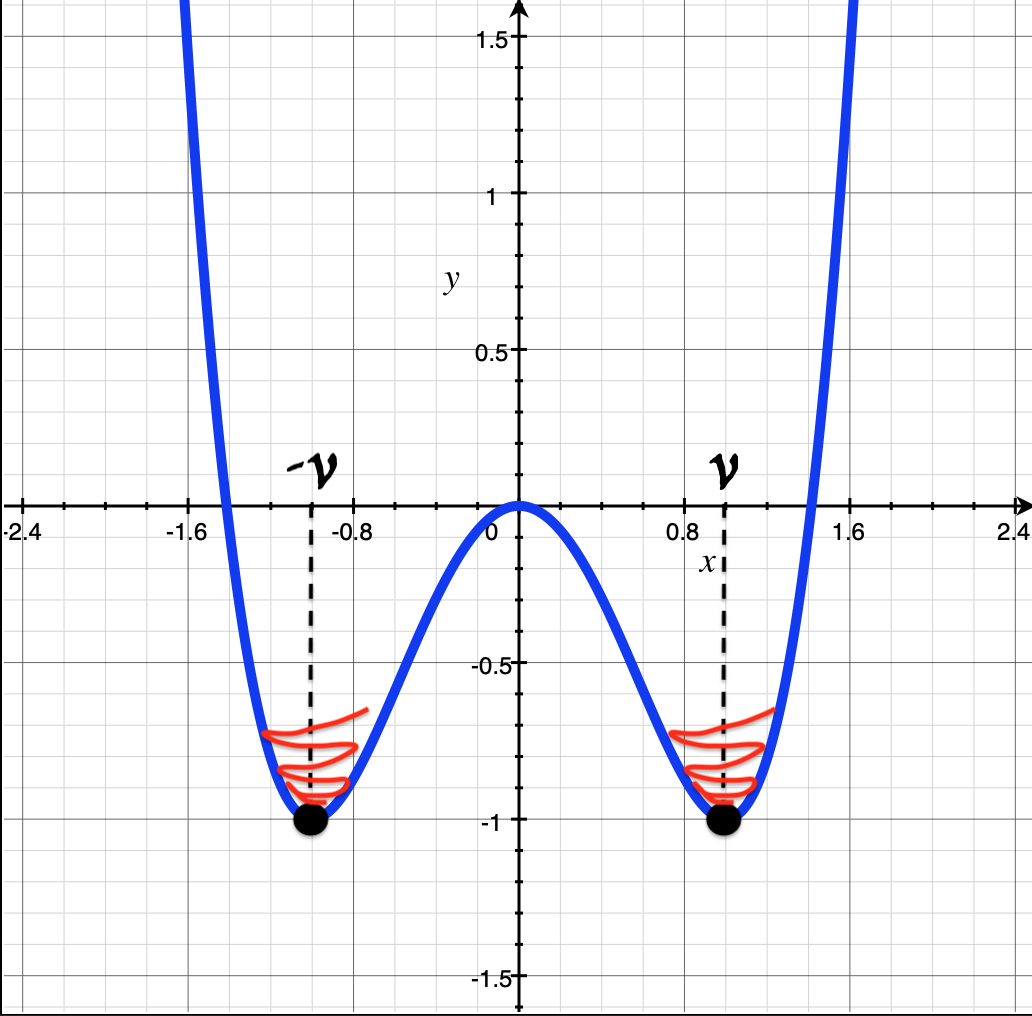
\includegraphics[width=2in]{images/mexhat2d_smalldev.png}
	\caption*{Small fluctuations in the energy behave much like the harmonic oscillator.}
\end{figure}

\noindent In the continuous case, we choose coordinates by rotating such that

\begin{equation}
\phi_0^j = \begin{pmatrix} 0 \\ 0 \\ \dots \\ \nu \end{pmatrix} = \begin{pmatrix} 0 \\ 0 \\ \dots \\ \frac{\mu}{\sqrt{\lambda}} \end{pmatrix}
\end{equation}

\noindent And see how this behaves with small energy fluctuations. Define \textit{shifted fields} in terms of some new coordinates where the vector of fields $\underline{\phi}$ is now defined as

\begin{equation}
\underline{\phi} (x) \equiv ( \pi^k (x), \nu + \sigma (x) ) \text{, where } k = 1, \dots , N-1.
\end{equation}

\noindent Note that $\pi$ is not the conjugate momentum density, but a new classical field, which will be, hence the notation, the pion, and $k$ denotes the vector index.

\noindent Rewrite $\mathcal{L}$ in terms of the shifted fields (\textbf{Exercise})

\begin{align}
\mathcal{L} = &\frac{1}{2} (\partial_\mu \pi^k)^2 + \frac{1}{2} (\partial_\mu \sigma)^2 \\
& - \frac{1}{2} \left( 2 \mu^2 \sigma^2 - \sqrt{\lambda} \mu \sigma^3 - \sqrt{\lambda} \mu (\pi^k)^2 \sigma - \frac{\lambda}{4} \sigma^4 - \frac{\lambda}{2} (\pi^k)^2 \sigma^2 - \frac{\lambda}{4} (\pi^k)^4 \right).
\end{align}

\noindent There are $N-1$ massless $\pi^k$ fields and one massive $\sigma$ field. The second and third terms in $\mathcal{L}$ correspond to an effective massive Klein-Gordon scalar field. The $N-1$ $\pi^k$ fields are effectively massless, as all of the other terms above contain $\lambda$ and are interaction terms. \\

\noindent It costs energy to move transverse in the potential, perpendicular to the circle of minima, corresponding to the effective mass of the $\sigma$ field. To move tangentially to the manifold of minima, the circle, it costs no energy, corresponding to the massless $\pi$ fields. \\

\subsubsection*{Goldstone's Theorem}

\noindent In the $O(N)$ linear $\sigma$-model there are ${N \choose 2}$ independent continuous symmetries, the dimension of the rotation group $O(N)$. After SSB, there are ${N-1 \choose 2}$ remaining symmetries, the dimension of $O(N-1)$, corresponding to rotations of the $\pi^k$ fields. The number of broken symmetries is equal to ${N \choose 2} - {N-1 \choose 2} = (N-1)$, which is also the number of massless fields. In other words, each broken symmetry causes a massless excitation: the \textit{Goldstone modes} or \textit{Goldstone bosons}. \\

\noindent \textbf{Therorem:} For every broken symmetry, there is a corresponding massless bosonic particle. \\

\noindent \textbf{Proof:} \\

\noindent Consider a classical field theory with fields $\phi^a (x)$, $a = 1, 2, \dots$, and the general Lagrangian density $\mathcal{L} = (\text{derivatives}) - V(\phi^a)$. \\

\noindent Let $\phi_0^a$ be a constant (in an extrema) field that minimizes the potential such that

\begin{equation}
\frac{\partial V(\phi^a)}{\partial \phi^a} \Big{|}_{\phi^a = \phi_0^a} = 0.
\end{equation}

\noindent Then expand the potential, a function of the vector of fields $\phi^a_0 \equiv \underline{\phi}_0$, near the minima

\begin{equation}
V(\phi^a) = V(\phi^a_0) + \frac{1}{2} (\phi^a - \phi_0^a) (\phi^b - \phi_0^b) \left( \frac{\partial^2 V}{\partial \phi^a \partial \phi^b} \right) \Big{|}_{\phi=\phi_0}.
\end{equation}

\noindent Call the Hessian matrix $[m^2]_{ab}$, which is symmetric and real and the eigenvalues give the masses of the effective fields. \\

\noindent With an orthogonal rotation, we can diagonalize a symmetric, real matrix $m^2 \rightarrow O^T D O$. Redefine the fields $\pi^a = [O]^a_b \phi^b$, and rewrite the Lagrangian density

\begin{equation}
\mathcal{L} (\pi^a) = (\text{derivatives}) - \sum_a D_a^2 (\pi^a)^2
\end{equation}

\noindent Where the eigenvalues correspond to the masses of the $\pi$ particles, and we must now show that there are eigenvalues equal to zero. In other words, every continuous symmetry leads to an eigenvalue equal to zero. \\

\noindent A general, global, continuous symmetry of the fields has the form

\begin{equation}
\phi^a \rightarrow \phi^a + \alpha \Delta^a (\phi)
\end{equation}

\noindent Where $\alpha$ is infinitesimal and $\Delta^a$ is a shift function of the fields. This is a symmetry of the potential, since it causes the derivatives to vanish such that

\begin{equation}
V(\phi^a) = V(\phi^a + \alpha \Delta^a (\phi)).
\end{equation}

\noindent This implies, by expanding and equating first order terms, the directional derivative of the potential is zero

\begin{equation}
\Delta^a (\phi) \frac{\partial}{\partial \phi^a} V(\phi) = 0.
\end{equation}

\noindent Differentiate this with respect to $\phi^b$ to get

\begin{equation}
\frac{\partial \Delta^a (\phi)}{\partial \phi^b} \frac{\partial V(\phi)}{\partial \phi^a} + \Delta^a (\phi) \frac{\partial^2 V}{\partial \phi^a \partial \phi^b} = 0.
\end{equation}

\noindent Evaluate at $\phi^a = \phi_0^a$ to get

\begin{equation}
\sum_a \Delta^a (\phi_0^a) [m^2]_{ab} = 0
\end{equation}

\noindent Where $\sum_a \Delta^a (\phi_0^a) = \Delta^T$ is the zero eigenvector, where the $\Delta^a (\phi^a_0)$ are linearly independent for each continuous symmetry, which follows by definition of the general, global, continuous symmetry imposed above.

\clearpage

\section{Lecture 17: The Higgs Mechanism}
\label{sec: lec17}

\noindent Here we discuss what happens when Goldstone's theorem related to spontaneous symmetry breaking (SSB) and local gauge invariance are combined. \\

\noindent Consider an $SU(2)$ gauge theory

\begin{equation}
\mathcal{L} = \bar{\psi} ( i \slashed{D} - m) \psi - \frac{1}{4} F_{\mu\nu} F^{\mu\nu}
\end{equation}

\noindent Where the second term represents the auxiliary gauge boson fields that are needed to induce the theory with local gauge invariance. \\

\noindent These (massive) gauge bosons are observed in experiment, and we are inclined to add a bosonic mass term to this theory. Naively, we can add a term of the form $\frac{1}{2} m^2 A_\mu^j (x) A_\mu^j (x)$. Unfortunately, this will break local gauge invariance since it does not obey the local gauge transformation like the gauge boson fields do, e.g., as $A_\mu^j (x) \rightarrow A_\mu^j (x) - \frac{1}{e} \partial_\mu \alpha (x)$. \\

\noindent The local gauge transformation is a \textit{constraint}, and constraints in physics can be solved by adding new degrees of freedom. For example, if we have $N$ equations (constraints) and $M$ unknowns (degrees of freedom), but $N >> M$, then there are no solutions! Therefore, we introduce new degrees of freedom until we get solutions, and, in the context of high energy physics, new degrees of freedoms are fields/particles/excitations! \\

\subsection*{Abelian case}

\noindent We consider the abelian case for the $SU(2)$ gauge theory combined with SSB as the ``toy'' model for such a theory. Consider a theory of a complex scalar field $\phi = \phi_R + i \phi_I$ (which can also be regarded as a doublet) coupled to a $U(1)$ gauge field $A_\mu$

\begin{equation}
\mathcal{L} = |D_\mu \phi |^2 - \frac{1}{4} F_{\mu\nu} F^{\mu\nu} - V(\phi)
\end{equation}

\noindent Where we have the covariant derivative $D_\mu = \partial_\mu + i e A_\mu$ obeying the local gauge condition. \\

\noindent We establish that $\mathcal{L}$ is indeed a gauge theory, since it is invariant under the local gauge transformation, since each term built from the invariant fields are invariant under local gauge transformation. The involved locally gauge invariant fields are

\begin{align}
A_\mu (x) &\rightarrow A_\mu(x) - \frac{1}{e} \partial_\mu \alpha (x) \\
\phi (x) &\rightarrow e^{i \alpha (x)} \phi (x).
\end{align}

\noindent For the interacting part of the theory, consider the potential

\begin{equation}
V(\phi) = -\mu^2 \phi^* \phi + \frac{\lambda}{2} (\phi^* \phi)^2 \text{, } \mu^2 > 0.
\end{equation}

\noindent Note that this potential is quartic in $\phi$, leaving no hope for solving this model straight away. To find a solution, we follow the same steps as for SSB: (1) Find a field value $\phi = \phi_0$ that minimizes the potential $V(\phi)$, and (2) expand the Lagrangian density around the minima and study small fluctuations in the field. \\

\noindent Following the same procedure as before, minimize $V(\phi)$ and we find the family of minima at (\textbf{Exercise}) $\phi_0 = e^{i \varphi} \sqrt{\frac{\mu^2}{\lambda}}$, and choose the $\varphi=0$ point, such that our minima occurs at 

\begin{equation}
\phi_0 = \sqrt{\frac{\mu^2}{\lambda}}.
\end{equation} 

\noindent To study small fluctuations about the minima, write the field as 

\begin{equation}
\phi (x) = \phi_0 + \frac{1}{\sqrt{2}} (\phi_1 (x) + i \phi_2 (x))
\end{equation}

\noindent Where $\phi_1$ and $\phi_2$ are small. Substituting into the potential, it becomes (\textbf{Exercise})

\begin{equation}
V(\phi) = -\frac{\mu^4}{2\lambda} + \mu^2 \phi_1^2 + \dots + \mathcal{O}(\phi_j^3)
\end{equation}

\noindent Where the $\dots$ account for all of the other terms form substituting $\phi(x)$, including $\phi_2$ terms and cross-terms of $\phi_1$ and $\phi_2$. Now expand $\mathcal{L}$ around the minima $\phi_0$ to get

\begin{equation}
\mathcal{L} = \frac{1}{2} |\partial_\mu \phi_1|^2 + \frac{1}{2} |\partial_\mu \phi_2|^2 - \mu^2 \phi_1^2 + \dots + \mathcal{O}(\phi_j^3).
\end{equation}

\noindent Note that other terms exist here, such as cross-terms, indicated by $\dots$, and that we alos have shifted away the constant terms in $\mathcal{L}$. The first two terms are effectively massless, while the third term is effectively massive, since it contains $\mu^2$. Other terms from the covariant derivative term include

\begin{equation}
|D_\mu \phi|^2 =  \frac{1}{2} |\partial_\mu \phi_1|^2 + \frac{1}{2} |\partial_\mu \phi_2|^2 + \sqrt{2} e \phi_0 A_\mu \partial^\mu \phi_2 + e^2 \phi_0^2 A_\mu A^\mu + \dots.
\end{equation}

\noindent We interpret the last term above as the \textit{bosonic mass term}

\begin{equation}
\Delta{\mathcal{L}} = e^2 \phi_0^2 A_\mu A^\mu \equiv \frac{1}{2} m_A^2 A_\mu A^\mu.
\end{equation}

\noindent This result is in the classical, low-energy limit, since we studied only small fluctuations of the field. \\

\noindent To outline the quantization of this theory, we use the path integral approach, although lattice quantization also works for this theory. So, break the Lagrangian density into free and interacting parts $\mathcal{L} = \mathcal{L}_0 + \mathcal{L}_{\text{int}}$, where

\begin{equation}
\mathcal{L}_0 = \frac{1}{2} |\partial_\mu \phi_1|^2 + \frac{1}{2} |\partial_\mu \phi_2|^2 - \mu^2 \phi_1^2 - \frac{1}{4} F_{\mu\nu} F^{\mu\nu}
\end{equation}

\noindent And $\mathcal{L}_{\text{int}}$ is the rest of the terms: perturbations leading to vertices in the Feynman rules. For example, in momentum space, one of the vertices looks like


\begin{figure}[H]\centering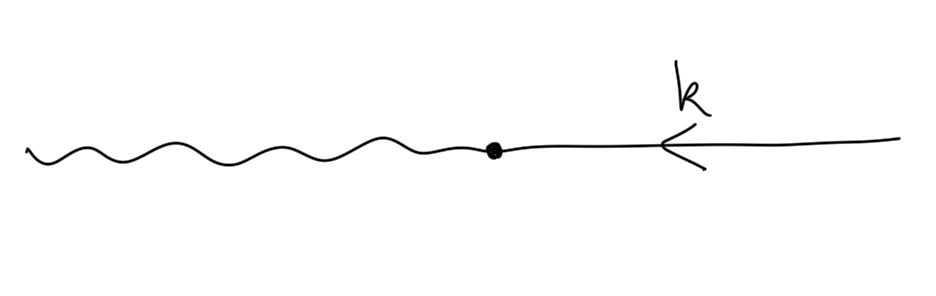
\includegraphics[width=2in]{images/ex_vertex.png} \end{figure} 
\begin{equation} = \sqrt{2} i e \phi_0 (-i k^\mu) \equiv m_A k^\mu \end{equation}

\noindent At the quantum level, the mass of the gauge boson fields manifest in the poles of the Green's functions. For example,


\begin{figure}[H]
	\centering
	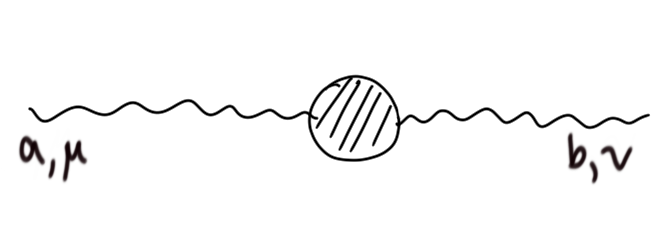
\includegraphics[width=2in]{images/gauge_boson_poles.png}
\end{figure} 
$$\sim$$
\begin{figure}[H]
	\centering
	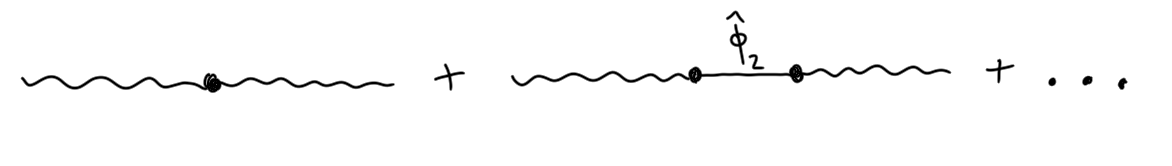
\includegraphics[width=3in]{images/gauge_boson_vertices.png}\end{figure} 
 \begin{equation} 
 = i m_A^2 g^{\mu\nu} + (m_A k^\mu) \frac{i}{k^2} (m_A k^\nu) \sim i m_A^2 
 \end{equation}
 
 \subsection*{Nonabelian case}
 
 \noindent For the nonabelian case of SSB in $SU(2)$ gauge theory, consider a general, continuous gauge group $\mathcal{G}$ and a set of scalar fields $\phi = \begin{pmatrix} \phi_1 \\ \vdots \\ \phi_d \end{pmatrix}$ that transform under the gauge group $\mathcal{G}$ as
 
 \begin{equation}
 \phi_j \rightarrow (\mathbb{I} + i \alpha^a t^a )_{jk} \phi_k
 \end{equation}
 
 \noindent Where $\alpha$ is small, such that we have the representation of an element $g \in \mathcal{G}$
 
 \begin{equation}
 \pi (g) = e^{i \alpha^a t^a}
 \end{equation}
 
 \noindent And the $\{t^a\}$ are purely imaginary matrices from the associated Lie algebra that depend on the representation. \\
 
 \noindent Now build a gauge theory based on the gauge group $\mathcal{G}$ by promoting it to a local symmetry that acts locally on the scalar fields as
 
 \begin{equation}
 \phi (x) \rightarrow \pi (g(x)) \phi (x).
 \end{equation}
 
 \noindent Derivatives of the scalar fields in this gauge theory will be the covariant derivative
 
 \begin{equation}
 D_\mu \phi = (\partial_\mu + g A_\mu^a \tau^a ) \phi
 \end{equation}
 
 \noindent Where the matrix $\tau^a = i t^a$. Build the kinetic energy terms by squaring and halving the covariant derivative acting on the field to obtain
 
 \begin{equation}
 \frac{1}{2} (\partial_\mu \phi_j )^2 + g A_\mu^a ( \partial_\mu \phi_j T_{jk}^a \phi_k ) + \frac{1}{2} g^2 A_\mu^a A^{b \mu} (\tau^a \phi)_j (\tau^b \phi)_j
 \end{equation}

\noindent Now introduce the aspect of SSB to this gauge theory by combining this with the wine bottle potential

\begin{equation}
V(\phi) = -\nu | \phi |^2 + \lambda | \phi |^4.
\end{equation}

\noindent So, there is a classical minima of these fields at $\phi_0$, such that $\phi (x) = \phi_0 + \epsilon \phi_1 (x)$, where $\phi_1 (x)$ are small fluctuations about the minima, which we substitute and expand about in the Lagrangian density to find terms like (\textbf{Exercise})

\begin{equation}
\Delta \mathcal{L} \sim \frac{1}{2} (m^2)_{ab} A_\mu^a A^{b \mu}
\end{equation}

\noindent Where we have a negative of a positive semidefinite matrix (if diagonable, then eigenvalues are $\ge 0$) with indices running from $a, \, b = 1, \dots, \text{dim}(\mathcal{G})$

\begin{equation}
(m^2)_{ab} \equiv g^2 (\tau^a \phi_0 )_j (\tau^b \phi_0)_j.
\end{equation}

\noindent For $\mathcal{G} = SU(2)$, choose the fundamental (spin-1) representation in terms of the Pauli spin matrices

\begin{equation}
\tau^1 = i \sigma^x, \,\,\,\,\,\,\,\, \tau^2 = i \sigma^y , \,\,\,\,\,\,\,\, \tau^3 = i \sigma^z.
\end{equation}

\noindent Then the fields (eigenvectors) in this basis are

\begin{equation}
\phi = \begin{pmatrix} \phi_1 \\ \phi_2 \end{pmatrix} \text{ and } \phi_0 = \begin{pmatrix} 1 \\ 0 \end{pmatrix}.
\end{equation}

\noindent The action of the generators $\tau^a$ on the minima, the vacuum state, are (\textbf{Exercise})

\begin{align}
\tau^1 \phi_0 &= i \begin{pmatrix} 0 \\ 1 \end{pmatrix} \\
\tau^2 \phi_0 &= - \begin{pmatrix} 0 \\ 1 \end{pmatrix} \\
\tau^3 \phi_0 &= i \begin{pmatrix} 1 \\ 0 \end{pmatrix} 
\end{align}

\noindent Giving matrix elements

\begin{equation}
[m^2] = g^2
\begin{bmatrix}
 -1 & -i & 0 \\
 -i & -1 & 0 \\
  0 & 0 & -1
\end{bmatrix}.
\end{equation}

\noindent If there is a generator $\tau^a$, in a different representation, that leaves the vacuum state invariant such that

\begin{equation}
\tau^a \phi_0 = 0
\end{equation}

\noindent Then there will be \textit{zero mass} terms (zero eigenvalues) in the matrix elements, indicating that initially massless bosons become massive when symmetry is broken! Specifically in the theory of electroweak interations, these particles are the $W^{\pm}$ and $Z$ bosons.

\clearpage

\section{Lecture 18: SSB with Gauge Theories and Next Steps}
\label{sec: lec18}

\noindent Here we complete our discussion of SSB in the context of gauge theories (e.g., the Higgs mechanism), and give a broad overview of open questions and where to go next. \\

\noindent Recall from the previous lecture we began working with a local gauge theory of bosons with a tuple of independent scalar fields $\begin{pmatrix} \phi_1 \\ \vdots \\ \phi_d \end{pmatrix}$. Each field transforms according to the local gauge symmetry

\begin{equation}
\phi_j \rightarrow (1 + i \alpha^a t^a)_{jk} \phi_k
\end{equation}

\noindent Where the $t^a$ is a purely imaginary representation. \\

\noindent Next, we added a potential to the Lagrangian density that is minimized by some configuration $\phi_0 = \text{arg}_{\phi} \text{min} (V(\phi))$. If this minimal configuration is not equal to zero $\phi_0 \ne 0$, then we can spontaneously generate mass. For example, we choose, via gauge invariance, an eigenvector with just one nonzero value to be the minimal configuration

\begin{equation}
\phi_0 = \begin{pmatrix} 0 \\ \vdots \\ \nu \end{pmatrix} \equiv \begin{pmatrix} \underline{0} \\ \nu \end{pmatrix}.
\end{equation}

\noindent To understand how the gauge bosons acquire mass, consider the kinetic energy term built with the covariant derivative mod squared $|D_\mu \phi |^2$, since the representation is purely imaginary, which is a long, complicated expression. Expand the fields in this expression around the minimal configuration by writing $\phi = \phi_0 + \phi_1$. This yields another long, complicated expression, but let's focus on the ``mass term'', which allows the spontaneous generation of mass in gauge theory,

\begin{equation}
|D_\mu \phi|^2 = \dots + \frac{1}{2} g^2 m_{ab}^2 A_\mu^a A^{b \mu}
\end{equation}

\noindent Where the mass matrix $m_{ab}^2$ is equal to

\begin{equation}
m_{ab}^2 = \begin{pmatrix} \underline{0} & \nu \end{pmatrix} \tau^a \tau^b \begin{pmatrix} \underline{0} \\ \nu \end{pmatrix}
\end{equation}

\noindent And can be positive semidefinite or negative semidefinite due to the metric. Consider the form of the gauge boson fields in this mass term

\begin{equation}
A_\mu^a A^{b \mu} = A^a_0 A^b_0 - A_1^a A_1^b - A_2^a A_2^b - A_3^a A_3^b   .
\end{equation}

\noindent The only non-negative term is the zeroth, timelike, longitudinal element, and will cause the entire term to not look like a mass term. The three spatial degrees of freedom in this expression, if $m^2_{ab}$ is positive semidefinite, will lead to a mass term in the Lagrangian density $\mathcal{L}$, since mass terms have a minus sign in $\mathcal{L}$. \\

\noindent The longitudinal term does not look right and can be cancelled off since, for the photon, momentum only has transverse components: no longitudinal components. Consider the vacuum polarization diagram like we sketched in the previous lecture for the Abelian Higgs model.

\begin{figure}[H]
	\centering
	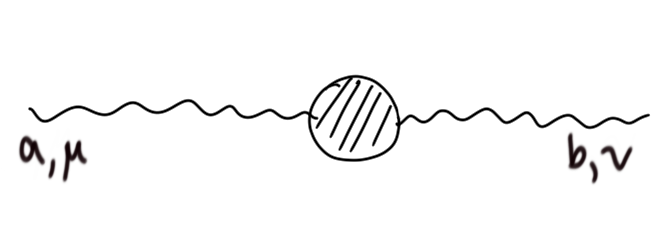
\includegraphics[width=2in]{images/gauge_boson_poles.png}
\end{figure} 

\noindent The contributing diagram in the propagation of a gauge boson, which cancels off the longitudinal term in the perturbation expansion, is a second order term involving the exchange of a fermion.

\begin{figure}[H]
	\centering
	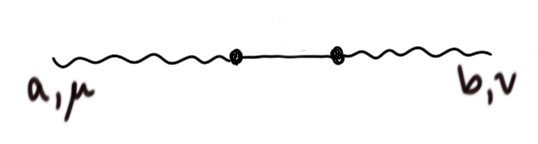
\includegraphics[width=2in]{images/gauge_boson_cancel.png}
\end{figure} 

\noindent This diagram contributes the \textit{purely transverse term}, with longitudinal contributions cancelled off,

\begin{equation}
i m_{ab}^2 \left( \eta^{\mu\nu} - \frac{k^\mu k^\nu}{k^2} \right).
\end{equation}

\noindent In the previous lecture, we worked out the fundamental representation of $SU(2)$ for the gauge theory. In this representation, work out the kinetic energy $\sim |D_\mu \phi|^2$ and find that

\begin{equation}
m_{ab}^2 \propto \mathbb{I}_{ab}.
\end{equation}

\noindent With the mass term proportional to the identity, this means that all three gauge bosons in this gauge theory have the same mass. Now, how do we build a gauge theory that gives mass to some gauge bosons but not others? \\

\subsection*{Glashow-Weinberg-Salam (GWS) Theory of Weak Interactions}

\noindent The GWS theory of weak interactions is a theory to describe gauge boson and electromagnetic field (photon) interactions in one theory. The local gauge group which this theory is invariant under is $SU(2) \times U(1)$. The gauge group symmetry transformations act on gauge boson fields as

\begin{equation}
\phi \rightarrow e^{i \alpha^a \tau^a} e^{i \frac{\beta}{2}} \phi
\end{equation}

\noindent Where $\tau^a = \frac{\sigma^a}{2}$ are the Pauli spin matrices from the $SU(2)$ (gauge boson) part of the group, and $\beta$ is a scalar from the $U(1)$ (photon) part of the group. Think of the action of $U(1)$ as giving charge to the field $\phi$. \\

\noindent Now add the potential $V(\phi)$ to the Lagrangian density and minimize the potential such that

\begin{equation}
\phi = \phi_0 + \phi_1 \, \text{ , where } \phi_0 = \frac{1}{\sqrt{2}} \begin{pmatrix} 0 \\ \nu . \end{pmatrix}
\end{equation}

\noindent Expand the covariant derivative around the minima $\phi_0$, and in the fundamental representation for this gauge group $SU(2) \times U(1)$, we get (\textbf{Exercise})

\begin{equation}
D_\mu \phi = (\partial_\mu - i g A_\mu^a \tau^a - \frac{i}{2} g' B_\mu ) \phi
\end{equation}

\noindent With the connection gauge field $\begin{pmatrix} A_\mu^a \\ B_\mu \end{pmatrix} \sim \begin{pmatrix} SU(2) \\ U(1) \end{pmatrix}$. Putting everything together into a locally gauge invariant Lagrangian density

\begin{equation}
\mathcal{L}_{\text{GWS}} = |D_\mu \phi|^2 - \frac{1}{4}F_{\mu\nu}F^{\mu\nu} + \dots + \text{fermion term} + \dots + V(\phi).
\end{equation}

\noindent The fermion term will be discussed below. \\

\subsubsection*{Mass Generation}

\noindent Due to the potential having a minimum configuration, we can generate mass in this gauge theory to endow gauge bosons with mass. We want to do this, because massive bosons are experimentally observed. Expand the Lagrangian density around the minima $\phi_0$ and acquire a term from the kinetic energy term that looks like (\textbf{Exercise})

\begin{equation}
\text{``mass term''} \equiv \frac{\nu^2}{8} \left( g^2 (A_\mu^1)^2 + g' (A_\mu^2)^2 + (ig A_\mu^3 + g' B_\mu)^2 \right).
\end{equation}

\noindent So, $A_\mu^1$,$ A_\mu^2$, and the combination of fields $A_\mu^3$/$B_\mu$ each act like they have a mass, interpreted as massive gauge bosons: three degrees of freedom from $SU(2)$. The fourth degree of freedom is missing from this mass term, and we, therefore, conclude that it does not have a mass, and we interpet this as the photon: one degree of freedom from $U(1)$. \\

\noindent It is convenient to rename the fields

\begin{align}
W_\mu^\pm &= \frac{1}{\sqrt{2}} \left( A_\mu^1 \mp i A_\mu^2 \right) \\
Z_\mu^0 &= \frac{1}{\sqrt{g^2 + g'^2}} \left( g A_\mu^3 - g' B_\mu \right)
\end{align}

\noindent With masses

\begin{align}
m_W &= \frac{1}{2} g \nu \\
m_Z &= \frac{1}{2} \sqrt{g^2 + g'^2} \nu.
\end{align}

\noindent The fourth field (degree of freedom), with zero mass, we call

\begin{equation}
A_\mu = \frac{1}{\sqrt{g^2 + g'^2}} (g' A_\mu^3 + g B_\mu ).
\end{equation}

\subsubsection*{Coupling to Fermions}

\noindent Gauge bosons couple differently to left-handed and right-handed fermions. Recall that the chirality of fermions arose in the development of gamma $\gamma$ matrices and Weyl spinors and the kinetic energy term decouples into

\begin{equation}
\bar{\psi} (i \slashed{\partial}) \psi = \bar{\psi}_L (i \slashed{\partial}) \psi_L + \bar{\psi}_R (i \slashed{\partial}) \psi_R.
\end{equation}

\noindent Similarly, in the gauge theory

\begin{equation}
\bar{\psi} (i \slashed{D}) \psi = \bar{\psi}_L (i \slashed{D}) \psi_L + \bar{\psi}_R (i \slashed{D}) \psi_R.
\end{equation}

\noindent To recognize this difference in chirality and coupling of gauge bosons to fermions, recall that we have the choice of representation of the gauge group $SU(2)$, and the left- and right-handed fermions can be separated into different representations.

\clearpage

\subsection*{Next Steps}

\noindent There are three ways to go from here:

\begin{enumerate}
\item Practical calculations for experiments, 
\item Physics-focused research,
\item Mathematics-focused research.
\end{enumerate}

\subsubsection*{Physics}

\begin{itemize}
\item Supersymmetry (SUSY)
	\subitem Upgrading symmetries of groups (e.g., Poincar\'e $\rightarrow$ Super Poincar\'e).
\item Quantum gravity via field theory tools (e.g., superstring theory, loop quantum gravity).
	\subitem Superstring theory offers a correct effective theory to explain the high energy physics of black holes.
\item Linear quantum gravity
	\subitem Does not lead to strings.
	\subitem Non-renormalizable theory.
	\subitem Treats the metric $g^{\mu\nu} = \eta^{\mu\nu} + \delta g^{\mu\nu}$ as the degree of freedom.
\item Linear quantum gravity with the Standard Model
	\subitem Only works up to some cutoff $\Lambda$, making an \textit{effective, low energy} theory of gravity. 
	\subitem Best theory we have to date for describing \textit{all} experiments, but we also believe that it is not fundamental, since black holes exist, which conflict with the imposed cutoff, and this theory fails at high energy predictions.
\item AdS/CFT Correspondence
	\subitem Exaplins quantum gravity with field theory alone, no strings.
	\subitem It states that a strongly interacting conformal quantum field theory (CFT) on the boundary of Anti-de Sitter spacetime (AdS) is dual to a quantum gravity theory of Anti-de Sitter spacetime (solutions to Einstein's equations) in its semiclassical limit, which implies that quantum gravity is itself a quantum field theory.
	\subitem We'd prefer to develop this theory in de Sitter spacetime, as that is the spacetime that we find ourselves in (see the work of Strominger).
\item Quantum information theory is becoming helpful to study the kinematics of quantum systems (e.g., photon entanglement).
\end{itemize}

\subsubsection*{Mathematics}

\noindent There are many rigorous formulations of quantum field theory:

\begin{itemize}
\item Axiomatic QFT,
\item Constructive QFT,
\item Functional integration, expansions, and probabilistic approaches,
\item Vertex operator algebras,
\item Chiral \& factorization algebras,
\item Topological QFT (TQFT) \& n-categories.
\end{itemize}

\noindent Why is QFT so difficult to make rigorous? \\

\noindent This is largely in part due to perturbation theory working so darn well, and it is used as the only \textit{standard} tool in QFT at large, but it is wrong, and we know why it is wrong. For example, consider a Gaussian path integral in a $(0+1)$-dimensional QFT with a quartic interaction $Z = \int_{-\infty}^\infty dx \, e^{-x^2 - g x^4}$. As prescribed, we assume that $g$ is small, do perturbation theory, get lots of terms, and end up with a zero radius of convergence! The interaction term does improve convergence, but perturbation theory can't see that. Even after Wick rotation of the path integral $Z = \int \mathcal{D} \phi \, e^{-S}$, which also improves convergence, perturbation theory can't calculate a finitie value for the path integral. Also note that for spacetime dimensions $d>6$, all QFTs are trivial (e.g., Gaussians). \\

\begin{itemize}
\item Axiomatic QFT
	\subitem Wightman: fields are distribution-valued objects (unbounded operators) acting on a Hilbert space.
	\subitem Hang-Kastler: $C^*$-algebras.
	\subitem Osterwalter-Schrader: statistical mechanical foundation (Wick-rotated).
	\subitem Reconstruction theorems: With all $n$-point correlation functions well-behaved, we can reconstruct full Hilbert space and the unitary representations of the Poincar\'e symmetry group.
	\subitem There are problems with local gauge theories (current research).
\item Constructive QFT
	\subitem Cluster expansions takes the Wick-rotated, Euclidean path integral and trade off the low energy perturbation series expansion for estimates of large values of the degrees of freedom that suppress bad parts of the series to get finite results.
	\subitem Successful in $(1+1)$- and $(2+1)$-dimensional spacetime, as well as local gauge theory, but it is very intricate and has become very difficult to communicate and check results.
\item Algebraic QFT
	\subitem Start with some axioms and abstract what the observables should be from there.
	\subitem Quantifies locality in the algebra, leading to observable ($C^*$) algebras.
	\subitem There is difficulty in finding the states ($n$-point function) to match the $C^*$ algebras.
\item Functional integration, expansions, and probabilistic approaches
	\subitem Nelson's axioms are stronger than the Osterwalter-Schrader axioms.
\item Vertex operator algebras
	\subitem Very successful with conformal field theories (CFTs), but is stuck in $(1+1)$ dimensions.
\item TQFT \& n-categories
	\subitem Exactly solvable, strongly interacting theories built on n-categories.
\item Chiral \& factorization algebras
	\subitem See the work of Costello on perturbation expansions.
\item Mathematical theory of effective QFT
	\subitem Follows the work of Wilson.
\end{itemize}



\clearpage
 
\end{document}

